\documentclass[final, english, english, a4paper, 12pt, numbers=noenddot, % Bei Änderung der Sprache 2 x kompilieren!
% tudscr spezifische Einstellungen
cd=false,
cdfont=false,cdfont=nohead,
cdmath=false,
cdhead=false,
cdfoot=true,
cdcover=monochrome,
cdgeometry=asymmetric,
declaration=heading,
declaration=notoc,
abstract=heading,
]{tudscrreprt}

%################ Hilfreiche Pakete laden #######################

%################ Hilfreiche Pakete laden #######################

\usepackage{settings/tudbwlimPackages}
\usepackage{settings/tudbwlimStyle}
\PassOptionsToPackage{hyphens}{url} % keep hyphen breaks even if 'url' sneaks in
\usepackage{xurl}                % generous breakpoints
\Urlmuskip=0mu plus 2mu             % a bit of stretch helps TeX find breaks
\urlstyle{same}
\usepackage{scrhack}
\usepackage{wrapfig}
\usepackage{microtype}
\usepackage{pgfplots}
\usepgfplotslibrary{fillbetween}
\pgfplotsset{compat=newest}
\usepackage{tikz}
\usetikzlibrary{arrows.meta,positioning,shapes.geometric,calc,fit, mindmap, matrix,shapes.multipart}
\usepackage{comment}
\usepackage{placeins}
\usepackage{multicol}
\usepackage{subcaption}
\usepackage{amssymb}
\usepackage{bm}
\usepackage{graphicx}
\usepackage[table]{xcolor} % allows coloring table cells
\usepackage{float}
\usepackage{xparse} % for \NewDocumentCommand
\usepackage{multirow}
\usepackage{array}
\usepackage{makecell}
\usepackage{autobreak}

%################ BIBLATEX #######################

\usepackage[bibencoding=auto,
        citestyle=authoryear-ibid,
        bibstyle=authoryear,
        backend = biber]{biblatex}% Vergessen Sie nicht in den Optionen das Bibliographieprogramm auf "biber" umzustellen! Um die Vorlage mit BibTeX nutzen zu können, muss die Option "backend=bibtex" übergeben werden. Es ist jedoch biber zu empfehlen, beachten Sie dazu die Hinweise der biblatex-Paketdokumentation im Abschnitt 3.15 "Using the fallback BibtTeX backend".
\usepackage{settings/BiblatexSetup}

%################ HYPEEREF #######################

\AfterPackage*{biblatex}%
{
        \RequirePackage[breaklinks=true, colorlinks=true, linktoc=section, linkcolor=blue, citecolor=black, hidelinks]{hyperref}
        % Da hyperref allerhand Veränderungen an vielen Standardbefehlen vornimmt, sollte dieses als letztes in der Präambel eingebunden werden. Nur Pakete, bei denen in der Dokumentation explizit darauf hingewiesen wird, dass diese nach hyperref zu laden sind, sollten auch danach folgen.
        \hypersetup{breaklinks=true}
        \hypersetup{pdfprintscaling=None} % gleiches Verhalten, auch ohne hyperref, liefert: \pdfcatalog{/ViewerPreferences<</PrintScaling/None>>}
        \usepackage{footnote} % https://tex.stackexchange.com/questions/207192/footcite-in-float-caption
        \makesavenoteenv{figure}
        \makesavenoteenv{table}
        \makesavenoteenv{algorithm}
}

\AfterPackage*{hyperref}
{
        \RequirePackage[automake,acronym,symbols,nomain,translate=babel]{glossaries}
        \usepackage{settings/GlossariesSetup}
}
%%%%%%%%%%%%%%%%%%%%%%%%%%%%%%%%%%%%%%%%%%%%%%%%%%%%%%%%%%%%%%%%%%%%%%%%%
%%%%%%%%%%%%%%%%%%%%%% LOADING FEASIBILITY CHECKS %%%%%%%%%%%%%%%%%%%%%%%
%%%%%%%%%%%%%%%%%%%%%%%%%%%%%%%%%%%%%%%%%%%%%%%%%%%%%%%%%%%%%%%%%%%%%%%%%
\definecolor{myblue}{RGB}{10,40,75}

\tikzset{
    line/.style   = {-Latex, very thick, draw=myblue, rounded corners=6pt},
    block/.style  = {draw=myblue, very thick, fill=blue!20,
            minimum width=3.5cm, minimum height=1.2cm,
            align=center, rounded corners=2pt},
    myDiamond/.style = {diamond, draw=myblue, very thick,
            minimum width=3cm, minimum height=2.5cm,
            aspect=1, align=center},
    decision/.style  = {myDiamond, fill=blue!20},
    decisionY/.style = {myDiamond, fill=yellow!80},
    decisionCP/.style = {myDiamond, fill=orange!80},
    dot/.style       = {circle, draw=myblue, very thick, fill=myblue,
            minimum size=8mm, inner sep=0pt},
}
%############## Own commands #####################´
\newcommand{\parbreak}{\vspace{\baselineskip}\noindent}
\newcommand{\gendreauDataSet}{Gendreau (2006)}
\newcommand{\mouraDataSet}{Moura (2009)}
\newcommand{\ceschiaDataSet}{Ceschia (2013)}
\newcommand{\krebsADataSet}{Krebs (2021a)}
\newcommand{\krebsBDataSet}{Krebs (2021b)}
\newcommand{\gendreauDataSetText}{\gendreauDataSet\ }
\newcommand{\mouraDataSetText}{\mouraDataSet\ }
\newcommand{\ceschiaDataSetText}{\ceschiaDataSet\ }
\newcommand{\krebsADataSetText}{\krebsADataSet\ }
\newcommand{\krebsBDataSetText}{\krebsBDataSet\ }


%Symbol macro: two stars
\newcommand{\twosym}{\ \(\bigstar\clubsuit\)}
%Symbol macro: two stars
\newcommand{\classsifiersym}{\ \(\bigstar\)}
%Symbol macro: two stars
\newcommand{\cpsym}{\ \(\clubsuit\)}

%Displaying hyperparameters better
\newcommand{\kv}[2]{\texttt{#1 = #2}}

% Helper macro for algorithmic lines with symbols
\newcommand{\BothState}[1]{\State #1\twosym}
\newcommand{\CPState}[1]{\State #1\cpsym}
\newcommand{\ClassifierState}[1]{\State #1\classsifiersym}

\newcolumntype{P}[1]{>{\centering\arraybackslash}m{#1}} % left-aligned p{} helper

% --- Convenience wrappers (put after your tikzset) ---
%\newcommand{\House}[3]{\pic {house={#1/#2/#3}};}                 % outlined house
%\newcommand{\Person}[3]{\pic {person={#1/#2/#3}};}               % outlined person
%\newcommand{\HouseFilled}[3]{\pic {house_filled={#1/#2/#3}};}    % filled house
%\newcommand{\PersonFilled}[3]{\pic {person_filled={#1/#2/#3}};}  % filled person


% ---------- Global style knobs ----------
\definecolor{numC}{RGB}{22,163,74} % green  (numerator)
\definecolor{denC}{RGB}{239,68,68} % red    (denominator)

% sizes (kept identical across all panels)
\newcommand{\ItemW}{0.8}   % item width
\newcommand{\ItemH}{0.6}   % item height
\newcommand{\ItemD}{0.8}   % item "depth/length"
\newcommand{\DistItemCont}{1.3}

\newcommand{\ContW}{2.3}   % container width
\newcommand{\ContH}{1.4}   % container height
\newcommand{\ContD}{1.4}   % container "depth/length"

% perspective offsets per unit depth (tweak once for the whole figure)
\newcommand{\dx}{0.52} % x-offset per unit depth
\newcommand{\dy}{0.35} % y-offset per unit depth

% ---------- Core drawing helpers ----------
% Draw a 2.5D cuboid from (x0,y0), with width w, height h, depth d.
% Fills/toplines are subtle; edges get a crisp outline.
\newcommand{\Cuboid}[7][]{% opts, x0, y0, w, h, d
    \begin{scope}[#1]
        \coordinate (A) at (#2,#3);
        \coordinate (B) at ($(A)+(#4,0)$);
        \coordinate (C) at ($(A)+(0,#5)$);
        \coordinate (D) at ($(A)+(#4,#5)$);
        \coordinate (S) at (\dx*#6,\dy*#6); % depth shift

        % Back rectangle (top) — light fill
        \fill[#7!3] ($(A)+(S)$) rectangle ($(D)+(S)$);

        % Front rectangle — a bit darker
        \fill[#7!6] (A) rectangle (D);

        % Connectors (sides)
        \fill[#7!10] (A) -- ($(A)+(S)$) -- ($(B)+(S)$) -- (B) -- cycle;       % bottom side
        \fill[#7!10] (B) -- ($(B)+(S)$) -- ($(D)+(S)$) -- (D) -- cycle;       % right side
        \fill[#7!10] (C) -- ($(C)+(S)$) -- ($(D)+(S)$) -- (D) -- cycle;       % top side

        % Crisp outlines (visible edges)
        \draw[black, line width=0.4pt] (A) rectangle (D);
        \draw[black, line width=0.4pt] (A) -- ($(A)+(S)$);
        \draw[black, line width=0.4pt] (B) -- ($(B)+(S)$);
        \draw[black, line width=0.4pt] (C) -- ($(C)+(S)$);
        \draw[black, line width=0.4pt] (D) -- ($(D)+(S)$);
        \draw[black, line width=0.4pt] ($(A)+(S)$) rectangle ($(D)+(S)$);
    \end{scope}
}

% Edge markers on one cuboid (placed on front-most edges).
%   width  = bottom-front edge
%   height = left-front vertical edge
%   length = right-leaning depth edge on top-front-right
\newcommand{\MarkWidth}[4]{% x0,y0,w,color
    \draw[line width=2.2pt, #4, rounded corners=0.6pt]
    (#1,#2) -- ++(#3,0);
}
\newcommand{\MarkHeight}[4]{% x0,y0,h,color
    \draw[line width=2.2pt, #4, rounded corners=0.6pt]
    (#1,#2) -- ++(0,#3);
}
% Mark the depth/length edge from top-right-front corner
\newcommand{\MarkLength}[4]{% x0,y0,d,color
    \coordinate (TRF) at (#1,0);%#2+\ItemH); % top-right-front
    \draw[line width=2.2pt, #4, rounded corners=0.6pt]
    (TRF) -- ++(\dx*#3,\dy*#3);
}

% Convenience wrappers that place item & container with consistent spacing
% They also expose anchors (I0,C0) for subsequent marks.
\newcommand{\PlaceItem}[2]{% x0,y0
    \coordinate (I0) at (#1,#2);
    \Cuboid{#1}{#2}{\ItemW}{\ItemH}{\ItemD}{black}
}
\newcommand{\PlaceContainer}[2]{% x0,y0
    \coordinate (C0) at (#1,#2);
    \Cuboid{#1}{#2}{\ContW}{\ContH}{\ContD}{black}
}

% ---------- Panel recipes ----------
% 1) Ratios between ITEM dimensions
\newcommand{\PanelItemDimDim}[3]{% cap, markA (W/H/L), markB (W/H/L), label
    \begin{subfigure}[t]{0.22\linewidth}
        \centering
        \begin{tikzpicture}[>=latex]
            \PlaceItem{0}{0}
            % choose axes for numerator/denominator
            % Numerator = green, Denominator = red
            \ifnum#2=1 \MarkWidth{0}{0}{\ItemW}{numC}\fi
            \ifnum#2=2 \MarkHeight{\ItemW}{0}{\ItemH}{numC}\fi
            \ifnum#2=3 \MarkLength{\ItemW}{0}{\ItemD}{numC}\fi

            \ifnum#3=1 \MarkWidth{0}{0}{\ItemW}{denC}\fi
            \ifnum#3=2 \MarkHeight{\ItemW}{0}{\ItemH}{denC}\fi
            \ifnum#3=3 \MarkLength{\ItemW}{0}{\ItemD}{denC}\fi
        \end{tikzpicture}
        \caption{#1}
    \end{subfigure}
}

% 2) Item vs Container dimension
\newcommand{\PanelItemVsCont}[2]{% caption, which axis: 1=W,2=H,3=L, label
    \begin{subfigure}[t]{0.32\linewidth}
        \centering
        \begin{tikzpicture}[>=latex]
            % place container slightly to the right
            \PlaceContainer{\DistItemCont}{0}
            \PlaceItem{0}{0}
            % numerator (item) green
            \ifnum#2=1 \MarkWidth{0}{0}{\ItemW}{numC}\fi
            \ifnum#2=2 \MarkHeight{\ItemW}{0}{\ItemH}{numC}\fi
            \ifnum#2=3 \MarkLength{\ItemW}{0}{\ItemD}{numC}\fi
            % denominator (container) red — marks drawn on its front edges
            \ifnum#2=1 \MarkWidth{\DistItemCont}{0}{\ContW}{denC}\fi
            \ifnum#2=2 \MarkHeight{\DistItemCont+\ContW}{0}{\ContH}{denC}\fi
            \ifnum#2=3 \MarkLength{\DistItemCont +\ContW}{0}{\ContD}{denC}\fi
        \end{tikzpicture}
        \caption{#1}
    \end{subfigure}
}

% 3) Height / Area  (area = item footprint W×L on front face surrogate)
\newcommand{\PanelHeightOverArea}[1]{%caption
    \begin{subfigure}[t]{0.22\linewidth}
        \centering
        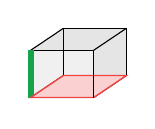
\begin{tikzpicture}
            \PlaceItem{0}{0}
            % numerator: height (green)
            \MarkHeight{0}{0}{\ItemH}{numC}
            % denominator: area (red) -> outline the front face footprint
            \fill[denC!25]
            (0,0) --
            (\ItemW,0) --
            (\ItemW+\dx*\ItemD, \dy*\ItemD) --
            (\dx*\ItemD,\dy*\ItemD) -- cycle;
            \draw[denC, line width=0.5pt]
            (0,0) --
            (\ItemW,0) --
            (\ItemW+\dx*\ItemD, \dy*\ItemD) --
            (\dx*\ItemD,\dy*\ItemD) -- cycle;
            % thin red frame on the front face
            \draw[black, line width=0.4pt] (\ItemW,0) -- (\ItemW,\ItemH);
            % thin red frame on the front face
        \end{tikzpicture}
        \caption{#1}
    \end{subfigure}
}

% 4) Area / Container Area
\newcommand{\PanelAreaOverContArea}[1]{%caption
    \begin{subfigure}[t]{0.35\linewidth}
        \centering
        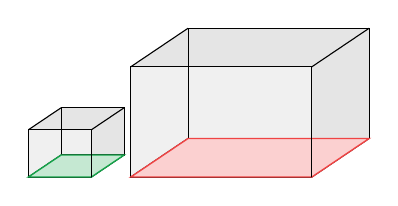
\begin{tikzpicture}
            \PlaceContainer{\DistItemCont}{0}
            \PlaceItem{0}{0}
            % numerator: item area (front face fill greenish)
            \fill[numC!25]
            (0,0) --
            (\ItemW,0) --
            (\ItemW+\dx*\ItemD, \dy*\ItemD) --
            (\dx*\ItemD,\dy*\ItemD) -- cycle;
            \draw[numC, line width=0.5pt]
            (0,0) --
            (\ItemW,0) --
            (\ItemW+\dx*\ItemD, \dy*\ItemD) --
            (\dx*\ItemD,\dy*\ItemD) -- cycle;
            \draw[black, line width=0.4pt] (\ItemW,0) -- (\ItemW,\ItemH);
            %Container  
            \fill[denC!25]
            (\DistItemCont,0) --
            (\ContW +\DistItemCont,0) --
            (\ContW+\DistItemCont+\dx*\ContD, \dy*\ContD) --
            (\dx*\ContD + \DistItemCont,\dy*\ContD) -- cycle;
            \draw[denC, line width=0.5pt]
            (\DistItemCont,0) -- (\ContW +\DistItemCont,0) -- (\ContW+\DistItemCont+\dx*\ContD, \dy*\ContD) -- (\dx*\ContD + \DistItemCont,\dy*\ContD) -- cycle;
            \draw[black, line width=0.4pt] (\ContW+\DistItemCont,0) -- (\ContW+\DistItemCont,\ItemH);
        \end{tikzpicture}
        \caption{#1}
    \end{subfigure}
}

% 5) Volume / Container Volume
\newcommand{\PanelVolumeOverContVolume}[1]{%caption
    \begin{subfigure}[t]{0.35\linewidth}
        \centering
        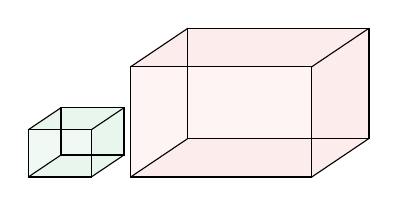
\begin{tikzpicture}
            \Cuboid{0}{0}{\ItemW}{\ItemH}{\ItemD}{numC}
            \Cuboid{\DistItemCont}{0}{\ContW}{\ContH}{\ContD}{denC}
        \end{tikzpicture}
        \caption{#1}
    \end{subfigure}
}

%################ Sonstige Einstellungen/Befehle #####################
\onehalfspacing

%################ Abkürzungen #######################
\makeglossaries % Glossar, Abkürzungsverzeichnis und Symbolverzeichnis erstellen
\glsenableentrycount % aktiviert \cgls, \cglspl, \cGls, \cGlspl, siehe https://tex.stackexchange.com/questions/98494/glossaries-dont-print-single-occurences/230664#230664

% Abkürzungen, die im Abkürzungsverzeichnis auftauchen und automatisch durch das glossaries-Paket sortiert werden
% ===============================
% Optimization & Problem Types
% ===============================
\newacronym[description={Container loading problem}]{CLP}{CLP}{container loading problem}
\newacronym[description={Pallet loading problem}]{PLP}{PLP}{pallet loading problem}
\newacronym[description={Bin packing problem}]{BPP}{BPP}{bin packing problem}
\newacronym[description={Strip packing}]{SP}{SP}{strip packing}
\newacronym[description={Cutting and packing}]{CaP}{C\&P}{cutting and packing}
\newacronym[description={Vehicle routing problem}]{VRP}{VRP}{vehicle routing problem}
\newacronym[description={Capacitated vehicle routing problem}]{CVRP}{CVRP}{capacitated vehicle routing problem}
\newacronym[description={Two-dimensional loading capacitated vehicle routing problem}]{2L-CVRP}{2L--CVRP}{two-dimensional loading capacitated vehicle routing problem}
\newacronym[description={Three-dimensional loading capacitated vehicle routing problem}]{3L-CVRP}{3L--CVRP}{three-dimensional loading capacitated vehicle routing problem}
\newacronym[description={Three-dimensional loading vehicle routing problem with time windows}]{3L-VRPTW}{3L--VRPTW}{three-dimensional loading vehicle routing problem with time windows}
\newacronym[description={Time windows}]{TW}{TW}{time windows}
\newacronym[description = {Relative percentage deviation}]{RDP}{RDP}{relative percentage deviation}

% ===============================
% Optimization Methods & Models
% ===============================
\newacronym[description={Linear programming}]{LP}{LP}{linear programming}
\newacronym[description={Mixed-integer programming}]{MIP}{MIP}{mixed-integer programming}
\newacronym[description={Constraint programming}]{CP}{CP}{constraint programming}
\newacronym[description={Lower bound}]{LB}{LB}{lower bound}
\newacronym[description={Upper bound}]{UB}{UB}{upper bound}

% ===============================
% Metaheuristics & Search Algorithms
% ===============================
\newacronym[description={Genetic algorithm}, plural=GAs, firstplural=genetic algorithms]{GA}{GA}{genetic algorithm}
\newacronym[description={Evolutionary algorithm}]{EA}{EA}{evolutionary algorithm}
\newacronym[description={Local search}]{LS}{LS}{local search}
\newacronym[description={Iterated local search}]{ILS}{ILS}{iterated local search}
\newacronym[description={Tabu search}]{TS}{TS}{tabu search}
\newacronym[description={Simulated annealing}]{SA}{SA}{simulated annealing}
\newacronym[description={Greedy randomized adaptive search procedure}]{GRASP}{GRASP}{greedy randomized adaptive search procedure}
\newacronym[description={Large neighborhood search}]{LNS}{LNS}{large neighborhood search}
\newacronym[description={Adaptive large neighborhood search}]{ALNS}{ALNS}{adaptive large neighborhood search}

% ===============================
% Packing Heuristics
% ===============================
\newacronym[description={Deepest-Bottom-Left-Fill}]{DBLF}{DBLF}{deepest-bottom-left-fill}
\newacronym[description={Bottom-Left-Fill}]{BLF}{BLF}{bottom-left-fill}
\newacronym[description={Maximum Touching Perimeter}]{MTP}{MTP}{maximum touching perimeter}
\newacronym[description={Maximum Touching Area}]{MTA}{MTA}{maximum touching area}
\newacronym[description={Last-in-first-out}]{LIFO}{LIFO}{last-in-first-out}
\newacronym[description={Manual last-in-first-out}]{MLIFO}{MLIFO}{manual last-in-first-out}
\newacronym[description={Load-bearing strength}]{LBS}{LBS}{load-bearing strength}
\newacronym[description={Loading Flag}, plural=LFLs]{LFL}{LFL}{loading flag}
\newacronym[description={Loading Status}]{LST}{LST}{loading status}

% ===============================
% Machine Learning & AI
% ===============================
\newacronym[description={Machine learning}]{ML}{ML}{machine learning}
\newacronym[description={Artificial neural network}]{ANN}{ANN}{artificial neural network}
\newacronym[description={Feedforward neural network}]{FFNN}{FFNN}{feedforward neural network}
\newacronym[description={Reinforcement learning}]{RL}{RL}{reinforcement learning}
\newacronym[description={Logistic regression}]{LR}{LR}{logistic regression}
\newacronym[description ={Extreme gradient boosting}]{XGB}{XGB}{extreme gradient boosting}
%\newacronym[description={Support vector machine}]{SVM}{SVM}{support vector machine}

% ===============================
% Evaluation Metrics (Confusion Matrix & ROC)
% ===============================
\newacronym[description={True Positive}]{TP}{TP}{true positive}
\newacronym[description={False Negative}]{FN}{FN}{false negative}
\newacronym[description={False Positive}]{FP}{FP}{false positive}
\newacronym[description={True Negative}]{TN}{TN}{true negative}
\newacronym[description={True Positive Rate}]{TPR}{TPR}{true positive rate}
\newacronym[description={False Positive Rate}]{FPR}{FPR}{false positive rate}
%\newacronym[description={Receiver Operating Curve}]{ROC}{ROC}{receiver operating curve}
\newacronym[description={Area Under The Receiver Operating Curve}]{AUROC}{AUROC}{area under the receiver operating curve}
\newacronym[description={Matthews Correlation Coefficient}]{MCC}{MCC}{matthews correlation coefficient}
\newacronym[description={Mutual Information}]{MI}{MI}{mutual information}
\newacronym[description={Fisher Score}]{F-Score}{F-Score}{fisher score}
\newacronym[description={Analysis of Variances}]{ANOVA}{ANOVA}{analysis of variances}
% Abkürzungen, die nicht im Abkürzungsverzeichnis aufgeführt werden
%\newabbreviation{zB}{z.\,B.}{zum Beispiel}

\glsaddall[types=abbreviation]

% Symbole die im Symbolverzeichniss erscheinen sollen
% Mit "F5" kompilieren oder "Tools -> Befehle -> makeglossaries" (F9) starten, um das Symbolverzeichnis zu aktualisieren
% \newsymb{<sort by>}{<name>}{<symbol>}{<unit>}
%
\begin{comment}
\newsymb{E}{Erwartungswert}{\mathbb{E}\left(\cdot\right)}{}
\newsymb{P}{Wahrscheinlichkeitsmaß}{\mathbb{P}\left(\cdot\right)}{}
\newsymb{V}{Varianz}{\mathbb{V}\left(\cdot\right)}{}
\newsymb{X}{Zufallsvariable}{X}{}
%
% Oder so verwenden und im Fließtext dann mit $\ExpValue$ arbeiten:
%\newcommand{\ExpValue}{\mathbb{E}\left(\cdot\right)}
%\newsymb{E}{Erwartungswert}{\ExpValue}{}
%
\glsaddall[types={symbols}] % Alle Symbole werden dem Symbolverzeichnis hinzugefügt
\end{comment}

%################ Bibliographie laden #######################
\addbibresource{./Diplomarbeit.bib} % Pfad/Name der .bib-Datei

%################ Ende Präambel #######################
\pagenumbering{Roman}

\makeatletter
\newcommand{\URLDiagnostics}{%
	\typeout{=== URL diagnostics ===}%
	\@ifpackageloaded{xurl}{\typeout{* xurl loaded}}{\typeout{* xurl NOT loaded}}%
	\@ifpackageloaded{url}{\typeout{* url loaded}}{\typeout{* url NOT loaded}}%
	\@ifpackageloaded{hyperref}{\typeout{* hyperref loaded}}{\typeout{* hyperref NOT loaded}}%
	\typeout{* breaklinks=\ifHy@breaklinks true\else false\fi}%
	\typeout{* url penalties: num=\the\value{biburlnumpenalty}, uc=\the\value{biburlucpenalty}, lc=\the\value{biburllcpenalty}}%
	\typeout{* Urlmuskip=\the\Urlmuskip}%
	\typeout{=== end URL diagnostics ===}%
}
\makeatother
\URLDiagnostics

\begin{document}
%################ Aufruf Deckblatt #######################
% mögliche Optionen, für weitere Informationen, siehe S. 23 des Benutzerhandbuchs des tudscr-Paket (http://mirrors.ctan.org/macros/latex/contrib/tudscr/doc/tudscr.pdf):

%%%%%%%%%%%%%%%%%%%%%%%%%%%%%%%%%%%%%
\thesis{\diplomathesisname}		% Diplomarbeit/Diploma-Thesis
%\graduation[Dipl.-Wirt. Ing.]{Diplom-Wirtschaftsingenieur} % [Dipl.-Kfm.]{Diplom-Kaufmann}
%
%\thesis{\masterthesisname}			% Master-Arbeit/Master Thesis
%\graduation[M.Sc.]{Master of Science}
%
%\thesis{\bachelorthesisname}		% Bachelor-Arbeit/Bachelor Thesis
%\graduation[B.Sc.]{Bachelor of Science}

%\renewcommand{\seminarCategoryText}{As part of the Industrial Management research seminar}
%\renewcommand{\seminarpapername}{Exposé}
%\newsavebox\thesisbox
%\savebox\thesisbox{\normalfont\large\sffamily \parbox{\textwidth}{\vspace{6pt} \raggedright \seminarCategoryText}}
% https://github.com/tud-cd/tudscr/issues/85 %
%
%\thesis{\seminarpapername \seminarCategory{\\\usebox\thesisbox}}		% Seminararbeit/Seminar Paper
%%%%%%%%%%%%%%%%%%%%%%%%%%%%%%%%%%%%%

\title{Learning-Based Algorithms for the Vehicle Routing Problem with Three-Dimensional Loading Constraints}
%\subtitle{Optionaler Unter-/Zusatztitel}
\author{%
	Maximilian Hubmann
	\matriculationnumber{4805234}
	\dateofbirth{21.03.2000}
	\placeofbirth{Nürnberg}
	\course{Industrial Engineering and Management}
}
\date[]{\today}
\supervisor{Dipl.-Wi.-Ing. Florian Linß}
\professor{Prof. Dr. Udo Buscher}

\setcounter{page}{1}

%%% IM 
\headlogo{./pictures/IM-Logo}
\faculty{Faculty of business and economics}
\chair{Chair of Business Administration, in particular Industrial Management}
\maketitle[cdtitle=true, cdfont=false]

%################ Abstract ######################
%\begin{abstract}
%These will be the sentences i will be most remembered for
%\end{abstract}

%%% Danksagung
%\danke{Danksagung}{Text}

%####################### Verzeichnisse ################%
%\microtypesetup{protrusion=false}
% Inhaltsverzeichnis
\tableofcontents

% Abbildungsverzeichnis (falls nichts benötigt, einfach als Kommentar setzen)
\listoffigures
\addcontentsline{toc}{chapter}{\listfigurename}

% Tabellenverzeichnis (falls nichts benötigt, einfach als Kommentar setzen)
\listoftables
\addcontentsline{toc}{chapter}{\listtablename}

% Algorithmenverzeichnis (falls nichts benötigt, einfach als Kommentar setzen)
%\listofalgorithms
%\addcontentsline{toc}{chapter}{\listalgorithmname}

\microtypesetup{protrusion=true}

%Abkürzungsverzeichnis (falls nichts benötigt, einfach als Blockkommentar setzen)
\printacronyms[style=bwlimsuper]
\addcontentsline{toc}{chapter}{\acronymname}

% Symbolverzeichnis (falls nichts benötigt, einfach als Blockkommentar setzen)
% \printsymbols[style=symblong, title=\listsymbolname]
% \addcontentsline{toc}{chapter}{\listsymbolname}



%############### Einstellungen für Fließtext setzen ####################
\clearpage
\setcounter{page}{1}\pagenumbering{arabic}

%####################### Fließtext ####################

\chapter{Introduction}
\label{sec:introduction}
In today’s globalized economy, efficient logistics networks are vital for managing the vast number of
goods transported daily. Maritime shipping, responsible for about $80\%$ of global trade,
forms a backbone of this network. \footcite[cf.][]{un_trade_and_development_unctad_review_2024}
However, the last mile, delivering individual parcels to customers, poses some of the most complex optimization
challenges. In 2022, over 161 billion parcels were delivered globally, equating to more than 5,000
deliveries every second.\footcite[cf.][]{statista_global_2022}
These numbers are only manageable through a strong logistics network, where even small inefficiencies
become very costly and optimization potential is huge. Two major challenges are faced in this domain, which
is the optimization of the routes driven by the delivery trucks, the \gls{VRP}, and the efficient arrangement of items
of various shapes and sizes, the \gls{CLP}. When the \gls{VRP} and the \gls{CLP} are solved integrated,
solutions are on average around $7\%$ better cost-wise, but are complex to solve as
both problems are $NP$-hard. \footcite[cf.][p. 23]{cote_value_2016} Therefore, efficient heuristics are the practical
choice to find good solutions in a reasonable time, because exact solution methods are limited to
small instances considering only few practical constaints, as orientation rules, stability, and load-bearing limits. \footcite[cf.][pp. 377--378]{bischoff_issues_1995}
Recent research has shown that \gls{ML} techniques can be used to accelerate the exact solution process
of the \gls{2L-CVRP}.\footcite[cf.][]{zhang_learning-based_2022}
Therefore this paper aims to provide an overview of the \gls{CLP} and explore how \gls{ML} can be used
to enhance the solution process of \gls{CLP} algorithms focusing on the \gls{3L-CVRP}.
The paper is structured as follows:
Chapter~\ref{chap:literature_review} introduces the \gls{CLP} and its common constraints, as well as classical
solution approaches. Promising \gls{ML} approaches will be discussed and a complete overview of algorithms
for \gls{3L-CVRP} algorithms will be conducted. The Chapter~\ref{chap:mathematical_formulation} introduces
a mathematical formulation for the \gls{3L-CVRP} and in the next Chapter~\ref{chap:classifier} the required
steps for developing a binary classifier are presented, ranging from data to modeling and the used features
are presented. Chapter~\ref{chap:algorithm} explains the implemented \gls{3L-CVRP} algorithm leveraging
the usage of the binary classifier and classical solution approaches. The computational results and the
tuning of the used parameters are shown in \ref{chap:computational_study} and this thesis ends with the conclusion
of the obtained results and the outlook fur further research steps in Chapter~\ref{chap:conclusion}.

\chapter{Literature Review}

\section{The Container Loading Problem}
\label{sec:clp_definition}

The placement and assignment of items to larger, mostly rectangular
containers, is a well known problem in logistics and operations research, as the
potential of cost savings and efficiency gains is substantial by reducing the number
of needed containers or by fulfilling customer needs. The \gls{CLP} covers a broad range of real-world applications,
such as loading cargo, optimizing warehouse storage and packing of pallets or cardboard boxes.
Generally it is differentiated in \textit{input minimization},
where the number of needed containers is minimized, and \textit{output maximization} problems,
where the value of the associated items is maximized. The \gls{BPP} is the generalized problem type of the \gls{CLP}
and belongs to \textit{input minimization} problems, whereas the knapsack problem to \textit{output maximization}. Apart from the expected outcome of the optimization,
the characterics of the items and containers is crucial for the problem definition. Items can be either
homogeneous or heterogeneous in size and shape. Furthermore, they can be classified as weakly or strongly
homogeneous or heterogeneous, depending on the degree of similarity among them. The container is
defined as a recangular volume with a fixed size and shape, where the items have to be placed in.
Other, non rectangular, shapes are seldomly considered in the literature, as the practical relevance is
limited. Multiple containers of homogeneous or heterogeneous sizes are used when the volume and weight
of the cargo require it.\footcite[cf.][pp. 1--2]{bortfeldt_constraints_2013}
According to \textcite{bischoff_issues_1995}, the mere placement of items in containers is insufficient
if practical requirements are not fulfilled as it lacks applicability. \footcite[cf.][pp. 1--2]{bischoff_issues_1995}
\textcite{bortfeldt_constraints_2013} systematically categorized all constraints emphasized in \gls{CLP} research
into five categories, which are presented in the following. They also distinguish between hard and soft constraints,
where hard constraints must be strictly satisfied, while soft constraints may be violated
to some extent.\footcite[cf.][p. 2]{bortfeldt_constraints_2013}  Figure~\ref{fig:solution-visualization}
visualizes a possible 3D packing with different constraints applied.

\begin{figure}[ht]
    \centering
    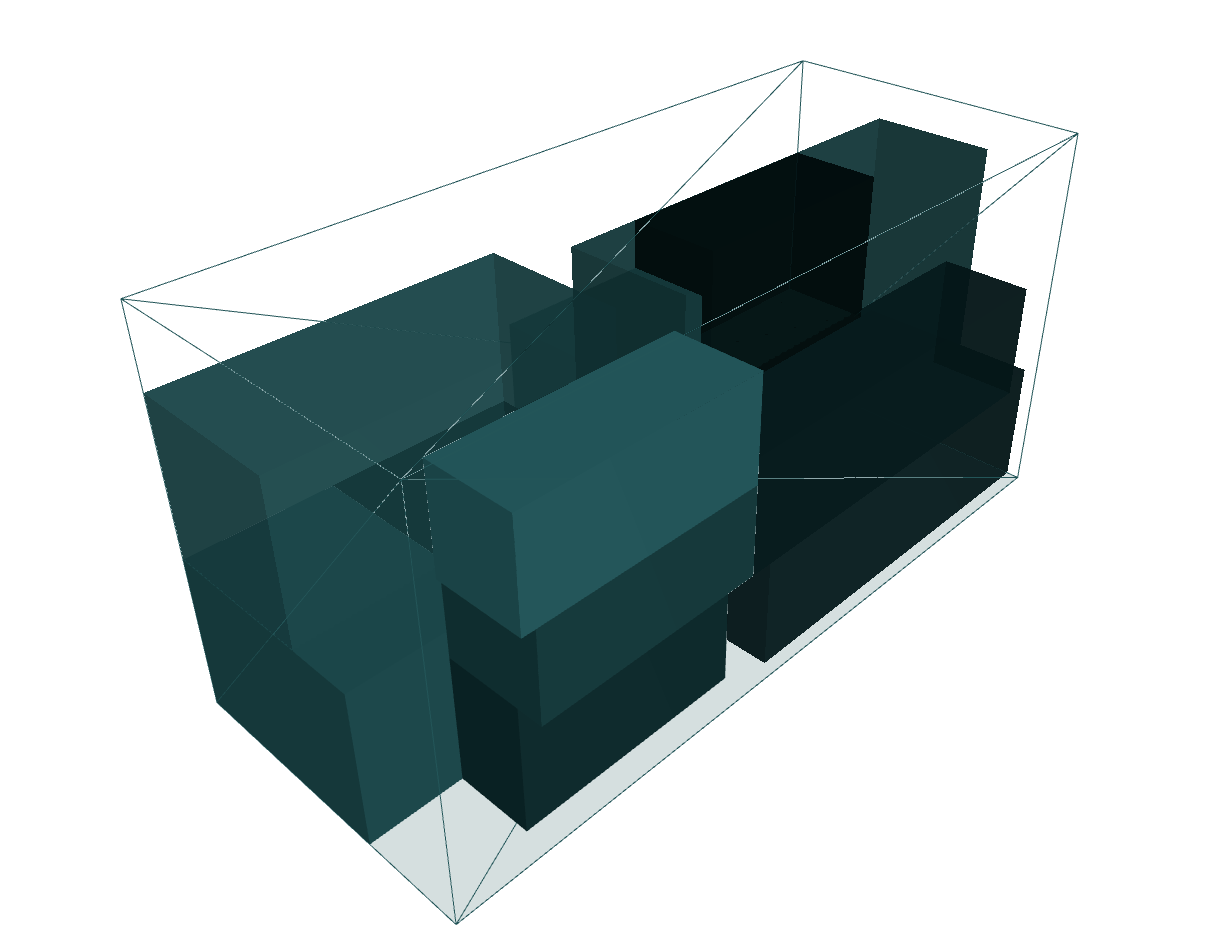
\includegraphics[width=6.3cm]{pictures/3l_cvrp_example.png}
    \caption[Visualized 3D packing with packing constraints.]{3D Packing with geometry, orthogonality and support area constraints.\footnotemark}.
    \footnotetext{CLP Visualizer from \textcite{tamke_branch-and-cut_2024}.}
    \label{fig:solution-visualization}
\end{figure}

\subsubsection{Container related constraints}
These constraints summarize all physical barriers of the container. The \textit{load capacity} limits the aggregated
mass of all items in the container. The distribution of the weight (\textit{load balance})
plays an important role for safety reasons, as the cargo must not move during the transport and the container
must not tip over and is defined by the maximum weight difference between the left and right half of the container.
When the containers are transported by trucks, uneven \textit{axle weight} distribution can cause severe
consequences and need to be avoided for practicability by loading the cargo axle-friendly. \footcite[cf.][pp. 849--850]{krebs_advanced_2021}

\subsubsection{Item related constraints}
Item related constraints define the properties of the item, which are relevant
for the packing. When the container capacity is limited (output maximization),
the \textit{loading priority} constraint defines the priority among possible
item candidates. The \textit{orientation} constraint restricts how an item can be rotated.
There are several types of rotation, each defined by the axis around which the item rotates.
The most common is the \textit{z-rotation}, where rotation is only allowed around the vertical axis.
When 3D packing is considered, stacking of items is allowed in comparison to 2D packing, when all
items are placed on the container floor. Two main approaches exist, when stacking is considered.
The \textit{fragility} constraint differentiates between fragile and non-fragile items,
allowing only non-fragile items to be stacked on non-fragile items. Figure \ref{fig:stacking_comparison} showcases
this definition. The other approach defines an individual \textit{\gls{LBS}} for each
item stating how much pressure the box can tolerate, and which items can be stacked. \footcite[cf.][pp. 847--848]{krebs_advanced_2021}

\begin{figure}[htbp]
    \centering
    \small
    % First TikZ picture
    \begin{subfigure}[b]{0.45\textwidth}
        \centering
        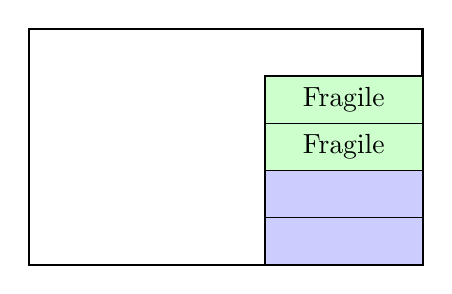
\begin{tikzpicture}
            % Draw the container
            \draw[thick] (0,0) rectangle (5,3);

            % Draw the three items inside
            \draw[fill=blue!20] (3,0) rectangle (5,0.6);
            \node at (4, 0.3) {};

            \draw[fill=blue!20] (3,0.6) rectangle (5,1.2);
            \node at (4, 0.9) {};

            \draw[fill=green!20] (3,1.2) rectangle (5, 1.8);
            \node at (4, 1.5) {Fragile};

            \draw[fill=green!20] (3,1.8) rectangle (5, 2.4);
            \node at (4, 2.1) {Fragile};

        \end{tikzpicture}
        \caption{Feasible stacking of items.}
    \end{subfigure}
    \hfill
    % Second TikZ picture
    \begin{subfigure}[b]{0.45\textwidth}
        \centering
        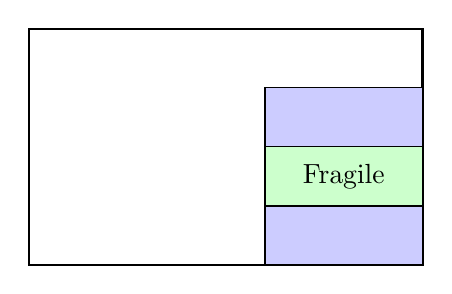
\begin{tikzpicture}
            \draw[thick] (0,0) rectangle (5,3);

            % Draw the three items inside
            \draw[fill=blue!20] (3,0) rectangle (5,0.75);
            \node at (4, 0.5) {};

            \draw[fill=green!20] (3,0.75) rectangle (5,1.5);
            \node at (4, 1.125) {Fragile};

            \draw[fill=blue!20] (3,1.5) rectangle (5, 2.25);
            \node at (4, 1.875) {};
        \end{tikzpicture}
        \caption{Infeasible stacking of items.}
    \end{subfigure}
    \caption[Visualization of fragility constraint.]{Comparison of fragile stacking (side view).}
    \label{fig:stacking_comparison}
\end{figure}


\subsubsection{Cargo-Related Constraints}
In contrast to item-related constraints, cargo-related constraints apply to
the entire cargo or to specific subsets of it. The \textit{complete-shipment} constraint
requires that all items within a shipment must either be loaded into the same
container or be left behind entirely. This constraint is important
when container capacity is limited (output maximization) and items
cannot be split. The \textit{allocation} constraint serves a similar purpose,
including the \textit{connectivity} constraint, which mandates that
certain items must be loaded into the same container, and the
\textit{separation} constraint, which requires specific items to
be distributed across different containers. For example, kitchen
shipments, comprising multiple packages, should be delivered together
to enable efficient installation. Conversely, items such as perfume and fresh
vegetables should be shipped separately due to incompatibility.

\subsubsection{Positioning constraints}

Positioning constraints determine, if items must be placed at
absolute locations or relative to other items. Absolute positioning is
typically based on item characteristics such as size, weight, or
content (e.g., bulky or hazardous items placed near the container door for accessibility) or
they may universally apply to all items, as the \textit{geometry} and
\textit{orthogonality} constraints. These constraints define that items are not allowed to overlap
and must be placed orhogonally to the container walls respectively.
Relative positioning requires items to be placed either close together as a \textit{group} or
\textit{separated} from each other.
The multi-drop constraint combines absolute and relative positioning requirements for items
destined for different delivery locations. The goal is to minimize reloading efforts by grouping items
by destination, arranging these groups in the delivery sequence, and applying either a \textit{\gls{LIFO}}
or sequential loading policy to ensure efficient unloading without having to move unrelated items.
Variations of the \gls{LIFO} constraint account for manual unloading (\textit{\gls{MLIFO}}) or unloading based on the
maximum allowable distance reachable from the unloading point (\textit{reachability}).

\subsubsection{Load-related constraints}

The \textit{stability} constraint is defined as one of the most critical constraints
in the \gls{CLP}, as it directly impacts the safety of both the cargo and the personnel involved.
First, a distinction must be made between \textit{horizontal} and \textit{vertical} stability.
Horizontal stability is achieved when items are securely connected to the
container walls or to other items, preventing lateral movement. Vertical
stability, on the other hand, is defined in various ways throughout the
literature. A common approach to assessing vertical stability is through the concept of the \textit{support
    area}, the portion of an item's base that rests on the surface below. Stability is typically
considered sufficient when the support area covers $75\%$ to $100\%$ of the item’s base. \footcite[cf.][p. 344]{gendreau_tabu_2006} However,
this may still result in unstable configurations if the center of gravity falls outside the
support area of the underlying layers, potentially causing the cargo to tilt. To improve practical stability,
a more reliable definition of vertical stability requires a minimum support area for all items below,
referred to as \textit{robust stability}.\footcite[cf.][p. 1140]{ceschia_local_2013} This comparison is illustrated in Figure~\ref{fig:vertical_stability_comparison}.
Additionally, it is crucial to ensure that the load remains stable even after partial unloading.
In addition, complexity constraints refer to specialized
requirements that are beyond standard packing rules. These include, for example, compatibility with automated or robot-assisted packing systems.

\begin{figure}[htbp]
    \centering
    \footnotesize
    % First TikZ picture
    \begin{subfigure}[b]{0.45\textwidth}
        \centering
        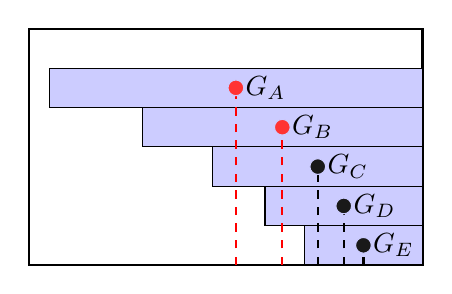
\begin{tikzpicture}
            % Draw the container
            \draw[thick] (0,0) rectangle (5,3);

            % Draw the three items inside
            % Draw the five items and their labels
            \draw[fill=blue!20] (3.5,0) rectangle (5,0.5);
            \draw[thick,dashed,black] (4.25,0) -- (4.25,0.25);  % <---
            \draw[fill = black!90, draw = blue!20] (4.25,0.25) circle (0.1);
            \node[anchor=west] at (4.25,0.25) {$G_E$};

            \draw[fill=blue!20] (3,0.5) rectangle (5,1);
            \draw[thick,dashed,black] (4,0) -- (4,0.75);  % <---
            \draw[fill = black!90, draw = blue!20] (4,0.75) circle (0.1);
            \node[anchor=west] at (4,0.75) {$G_D$};

            \draw[fill=blue!20] (2.33,1) rectangle (5,1.5);
            \draw[thick,dashed,black] (3.67,0) -- (3.67,1.25);  % <---
            \draw[fill = black!90, draw = blue!20] (3.67,1.25) circle (0.1);
            \node[anchor=west] at (3.67,1.25) {$G_C$};

            \draw[fill=blue!20] (1.44,1.5) rectangle (5,2);
            \draw[thick,dashed,red] (3.22,0) -- (3.22,1.75);  % <---
            \draw[fill=red!80, draw = blue!20] (3.22,1.75) circle (0.1);
            \node[anchor=west] at (3.22,1.75) {$G_B$};

            \draw[fill=blue!20] (0.26,2) rectangle (5,2.5);
            \draw[thick,dashed,red] (2.63,0) -- (2.63,2.25);  % <---
            \draw[fill=red!80, draw = blue!20] (2.63,2.25) circle (0.1);
            \node[anchor=west] at (2.63,2.25){$G_A$};


            %\node at (4, 1.875) {Fragile};
            %\node[anchor = west,align=center] at (2.9,2.5) {\small Center of \\  balance};

        \end{tikzpicture}
        \caption{Feasible, but unrobust, stacking with 75\% support area.}
    \end{subfigure}
    \hfill
    % Second TikZ picture
    \begin{subfigure}[b]{0.45\textwidth}
        \centering
        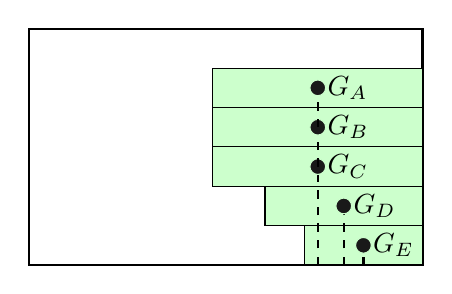
\begin{tikzpicture}
            % Draw the container
            \draw[thick] (0,0) rectangle (5,3);
            % Draw the three items inside
            % Draw the five items and their labels
            \draw[fill=green!20] (3.5,0) rectangle (5,0.5);
            \draw[thick,dashed,black] (4.25,0) -- (4.25,0.25);  % <---
            \draw[fill = black!90, draw = green!20] (4.25,0.25) circle (0.1);
            \node[anchor=west] at (4.25,0.25) {$G_E$};

            \draw[fill=green!20] (3,0.5) rectangle (5,1);
            \draw[thick,dashed,black] (4,0) -- (4,0.75);  % <---
            \draw[fill = black!90, draw = green!20] (4,0.75) circle (0.1);
            \node[anchor=west] at (4,0.75) {$G_D$};

            \draw[fill=green!20] (2.33,1) rectangle (5,1.5);
            \draw[thick,dashed,black] (3.67,0) -- (3.67,1.25);  % <---
            \draw[fill = black!90, draw = green!20] (3.67,1.25) circle (0.1);
            \node[anchor=west] at (3.67,1.25) {$G_C$};

            \draw[fill=green!20] (2.33,1.5) rectangle (5,2);
            \draw[thick,dashed,black] (3.67,1.25) -- (3.67,1.75);  % <---
            \draw[fill = black!90, draw = green!20] (3.67,1.75) circle (0.1);
            \node[anchor=west] at (3.67,1.75) {$G_B$};

            \draw[fill=green!20] (2.33,2) rectangle (5,2.5);
            \draw[thick,dashed,black] (3.67,1.75) -- (3.67,2.25);  % <---
            \draw[fill = black!90, draw = green!20] (3.67,2.25) circle (0.1);
            \node[anchor=west] at (3.67,2.25) {$G_A$};


            %\node at (4, 1.875) {Fragile};
            %\node[anchor = west,align=center] at (2.9,2.5) {\small Center of \\  balance};

        \end{tikzpicture}
        \caption{Feasible and robust stacking regarding 75\% support area.}
    \end{subfigure}
    \caption[Comparison of different vertical stability constraints.]{Comparison of different vertical stability constraints \\ with G = Center of Gravity (container side view). \footnotemark}
    \footnotetext{Own figures based on \textcite[p. 845]{krebs_advanced_2021}.}
    \label{fig:vertical_stability_comparison}
\end{figure}



\section{Classical Solution Approaches}
\label{sec:classical_solution_approaches}
The \gls{CLP} is a NP-hard combinatorial problem. \footcite[cf.][p. 11]{bortfeldt_constraints_2013}
Consequently, heuristics and metaheuristics were the dominating tools
in the early stages of this research field.\footcite[cf.][]{pisinger_heuristics_2002} The variety of methods
and their solution quality for solving the 2D \gls{CLP} developed in recent years. \footcite[cf.][p. 23]{iori_exact_2021}
The variety of 3D algorithms, especially for exact methods, is in comparison limited, as
\textcite{zhao_comparative_2016} elaborated in their survey. The following Figure~\ref{fig:solution_methods_overview}
presents this overview of the solution methods for the 3D \gls{CLP}.\footcite[cf.][]{zhao_comparative_2016}
It is divided in three categories constructive heuristics, metaheuristics
and exact methods. Hybrid methods and improvement heuristics are not explicitly shown in the figure,
as the former combines components from multiple categories, while the latter is subsumed within
metaheuristics. The depicted solution methods are described in the following.

\begin{figure}[htbp]
    \centering
    \resizebox{0.55\linewidth}{!}
    {
        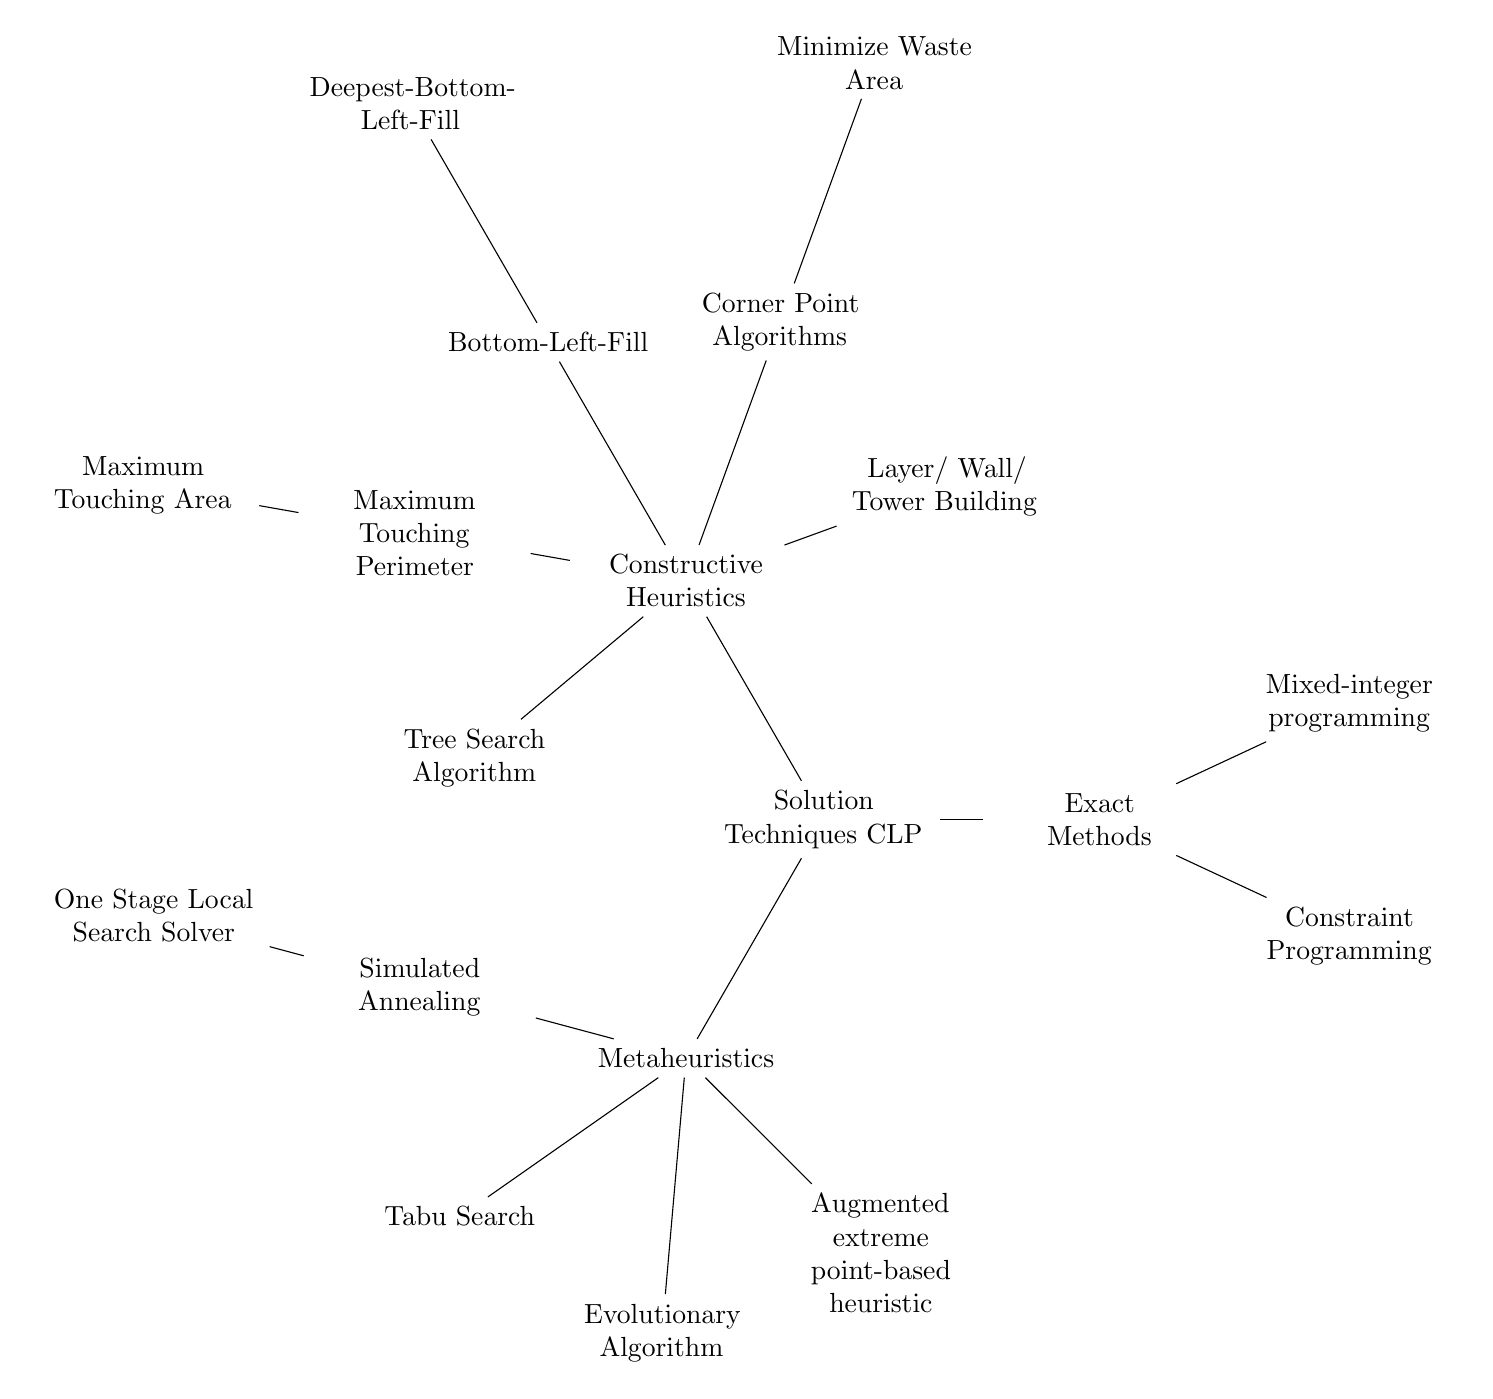
\begin{tikzpicture}[grow cyclic, text width=2.7cm, align=flush center,
                level 1/.style={level distance=3.5cm,sibling angle=120},
                level 2/.style={level distance=3.5cm,sibling angle=50}
            ]

            \node {Solution Techniques \gls{CLP}}
            child { node {Metaheuristics}
                    child { node {Simulated Annealing}
                            child{node{One Stage Local Search Solver}}}
                    child { node {Tabu Search}}
                    child { node {Evolutionary Algorithm}}
                    child { node {Augmented extreme point-based heuristic}}
                }
            child { node {Exact \\ Methods}
                    child { node {Constraint Programming}}
                    child { node {Mixed-integer programming}}
                }
            child { node {Constructive Heuristics}
                    child { node {Layer/ Wall/ Tower Building}}
                    child { node {Corner Point Algorithms}
                            child{node{Minimize Waste Area}}}
                    child { node {Bottom-Left-Fill}
                            child{node{Deepest-Bottom-Left-Fill}}}
                    child { node {Maximum Touching Perimeter}
                            child{node{Maximum Touching Area}}}
                    child { node {Tree Search Algorithm}}
                }
            ;

        \end{tikzpicture}
    }
    \caption{Overview of solution methods for the container loading problem.}
    \label{fig:solution_methods_overview}
\end{figure}



\subsubsection{Constructive Heuristics}
For obtaining an initial feasible solution, two primary strategies are commonly
used depending on the heterogeneity of the items. In cases where the items are weakly homogeneous,
the problem dimensionality is reduced from 3D to 2D by constructing either
\textit{walls} or \textit{layers} of similarly sized items. These structures fill one
dimension of the container, typically either length and height or width and length, thereby
simplifying the remaining problem space. Moreover, when the layers or walls have
equal dimensions approximately, horizontal and vertical stability constraints are met.
Beyond these two dominant approaches, several adaptations exist to address item heterogeneity.
For example, \textcite{gehring_genetic_1997} propose the construction of item
\textit{towers}, in which boxes are stacked on top of other items so that the base of the box is covered completely
by the box below it.
This effectively reduces the dimensions from 3D to a 2D floor space arrangement,
similar to the \gls{PLP}. \footcite[cf.][pp. 402--406]{gehring_genetic_1997}
Another method involves forming \textit{blocks} composed of identically shaped items.
These blocks are treated as single entities
during packing, significantly reducing the number of elements to be handled and thus
lowering overall problem complexity.\footcite[cf.][p. 801]{liu_novel_2011} Even though constructive heuristics are quite simple,
they are still widely used because of their simplicity and efficiency to obtain fast solutions.
\footcite[cf.][pp. 11--13]{tamke_branch-and-cut_2024}

\subsubsection{Metaheuristics}
Once an initial solution is found, metaheuristics or improvement heuristics can be applied
to improve it. Therefore a solution representation, such as a permutation of items, is required
to conduct changes of the current solution. \gls{GA}s were
used to either improve the walls, towers or layers found by the constructive heuristics
or by improving the quality of the permutation of all items. \footcite[cf.][]{gehring_genetic_1997}
\gls{TS} is a widely used approach for \gls{BPP} and \gls{CLP}. It is based on
the idea of iteratively improving a solution by exploring its neighborhood and simultaneously
storing certain moves or complete solutions in a tabu list to avoid back-cycling to
previous solutions, feasible or infeasible ones. \footcite[cf.][pp. 344--345]{gendreau_tabu_2006} \gls{SA} has rarely been used as a
standalone metaheuristic in the context of \gls{CLP}. Instead, it is often combined
with other approaches to leverage its cooling schedule, which allows the acceptance of
worse solutions at higher temperatures. This helps the algorithm to escape local optima
early in the search and gradually transition into a more focused intensification phase as
the temperature decreases. \gls{GRASP} has the advantage of controlling the selection of new
cuboid candidates along a spectrum between completely random and full greedy choices. \footcite[cf.][]{moura_grasp_2005}

\subsubsection{Exact Algorithms}
Retrieving optimal solutions for the \gls{CLP} is computationally challenging in comparison
to finding good solutions with heuristics. The main difficulty is to represent packing
patterns and the constraints introduced in Chapter~\ref{sec:clp_definition} in a mathematical way.
Two prominent methods exist for modeling the \gls{CLP}. The first one is \gls{MIP}, which can be
formulated in two primary ways. One approach defines each possible packing pattern as
a variable. \footcite[cf.][pp. 29--30]{zhu_prototype_2012} The second approach models
the placement of items using discrete coordinate variables. \footcite[cf.][pp. 4--8]{moura_integrated_2009}
Both formulations can benefit from enhancements such as branch-and-price or branch-and-cut
methods, which reduce the search space and improve solution time.
The second main method is \gls{CP}, which offers a flexible alternative for handling
complex constraints, where the focus is to find feasible solutions primarily and
not fulfilling an optimization criterion directly. \footcites[cf.][pp. 5--8]{kucuk_constraint_2022}[cf.][pp. 7--11]{tamke_branch-and-cut_2024} \textcite{iori_exact_2021} states, that
\gls{CP} improved the results of 2D \gls{CLP} problems significantly and is a promising
field of future research.\footcite[cf.][p. 23]{iori_exact_2021}

\parbreak

In general exact methods are not capable of solving large instances with practical relevance
in reasonable computation time. However, they can be used to understand the structure
of optimal solutions to provide lower bounds and guidance for the development of future
heuristics. \footcite[cf.][p. 2]{tamke_branch-and-cut_2024} A possible approach to improving
the performance of exact algorithms is the use of speed-ups, such as pretrained \gls{ML} models.
These models can substitute parts of the algorithm's computation time by predicting solution
feasibility or by quickly identifying good solutions, thereby reducing the need for exact instance
solving in iterative procedures, as will be further discussed in the next chapter.

\section{Motivation for Feasibility Prediction}
\label{sec:motivation_feasibility_prediction}
This section explores how \gls{ML} algorithms can enhance \gls{CLP} solution strategies,
highlighting both benefits and limitations. Two papers will be
analyzed, which use predictive methods to accelerate the computation time. Before that,
a short introduction to classifiers will be conducted. It is important to note that
several \gls{ML} approaches address the \textit{on-line} \gls{BPP}, where the optimal placement
of individual items, arriving sequentially, must be determined.\footcite[cf.][p. 1]{ali_-line_2022}
Since this work focuses on the \textit{off-line} \gls{BPP}, where a placement for all items is determined
simultaneously, on-line approaches are not further considered. The emphasis is placed primarily
on \gls{ML}-based classifiers. These are supervised \gls{ML} algorithms predicting the
value of a categorical or binary output column, called label, based on the
values of other columns, called features. Classifiers learn from a labeled dataset,
where the correct output values are known in advance, and then use this knowledge to
make predictions on new, unseen data. The accuracy can be evaluated afterwards by comparing
the predicted labels with the actual labels. \footcite[cf.][]{kotsiantis_supervised_2007}
An exemplary train dataset is shown in Table~\ref{tab:classifier_label_data}.

\begin{table}[ht]
    \small
    \centering
    \begin{tabular}{@{}cccccc@{}}
        \toprule
        \textbf{Instance} & \textbf{Feature 1} & \textbf{Feature 2} & \dots  & \textbf{Feature n} & \textbf{Label} \\
        \midrule
        1                 & xxx                & x                  & \dots  & xx                 & True           \\
        2                 & xxx                & x                  & \dots  & xx                 & False          \\
        3                 & xxx                & x                  & \dots  & xx                 & True           \\
        \vdots            & \vdots             & \vdots             & \vdots & \vdots             & \vdots         \\
        \bottomrule
    \end{tabular}
    \caption[Exemplary training dataset for a classifier with known labels.]{Exemplary training dataset for a classifier with known labels. \footnotemark}
    \footnotetext{Adapted table from \textcite[p. 249]{kotsiantis_supervised_2007}.}
    \label{tab:classifier_label_data}
\end{table}


A classifier can be implemented using various \gls{ML} models such as \gls{LR},
\gls{ANN}, support vector machine, or others. However, the most crucial aspect of any
\gls{ML} model is the selection of data, particularly the choice of features and
the size of the training set, since many models can be easily preselected from available
libraries and be compared performance wise. The model attempts to learn correlations between the provided features
and the corresponding labels. If the features are poorly chosen, the model may fail
to capture the underlying patterns in the data. Additionally, if the training set
is too small, the model might not generalize well, ultimately lacking the ability
to accurately predict unseen data. Furthermore, it needs to be noted, that available
\gls{ML} models are not by nature superior to other models, but can significantly outperform
other models on specific application problem \footcite[cf.][pp. 250, 264]{kotsiantis_supervised_2007}.


\subsection{Objectices for ML approaches}
To compare different models and \gls{ML} approaches idetnical objectives are needed. The most common
measures rely on the output of the confusion matrix, which sorts the output along
their true and predicted labels.

\begin{table}[ht]
    \centering
    \begin{tabular}{@{}lcc@{}}
        \toprule
                                 & \textbf{Predicted Positive} & \textbf{Predicted Negative} \\
        \midrule
        \textbf{Actual Positive} & True Positive (TP)          & False Negative (FN)         \\
        \textbf{Actual Negative} & False Positive (FP)         & True Negative (TN)          \\
        \bottomrule
    \end{tabular}
    \caption{Confusion matrix (binary classification).}
    \label{tab:confusion_matrix}
\end{table}
The output can be used to calculate the accurac and F1 scote of the classification, which
helps to interpret the outcomes and compare different model types.

\[
    \text{Accuracy}=\frac{TP+TN}{TP+TN+FP+FN}
    \qquad
    \text{F1}=\frac{2\,TP}{2\,TP+FP+FN}
\]


The usage of classifiers is promising to complement exisiting algorithms, as shown in the following.


\subsubsection{Feasibility Classifier of the \cgls{2L-CVRP}}
A practical application of the \gls{CLP} is the integration in the \gls{VRP}, where
a number of customers need to be served with a set of items by a fleet of vehicles that have
to start from a depot and return. The goal is to minimize the total distance driven
by the vehicles. When considering multidimensional items, the NP-hard problem itself,
increases in complexity, as every tour is representing a \gls{CLP} itself. \footcite[cf.][pp. 1--2]{tamke_branch-and-cut_2024}
\textcite{zhang_learning-based_2022} used a binary classifier to predict the feasibility of the
loading of single tours to reduce the overall computation time in their exact branch-and-price
algorithm. As many single tours need to be evaluated, the \gls{FFNN} model, a special type of \gls{ANN} models, reduced the need
to control the solutions only when they are discarded or accepted. The default approach would be to
determine feasibility by applying a exact feasibility checker, such as a \gls{CP} or \gls{MIP} model.
The classifier performed well and had an accuracy of at most $94.1\%$. However, some simplifications were made,
they allowed no stacking of items tackling the \cgls{2L-CVRP} and no further constraints,
as unloading sequence, rotation or stability (see Chapter~\ref{sec:clp_definition}) were considered.
The classifier was trained with a dataset of 50,000 tours obtained by the underlying column generation
algorithm containing 17 hand-crafted features capturing geometric
and spatial characteristics of the packing problem. These include the ratio of the total item area
to the container floor area, as well as the mean, standard deviation, minimum, and maximum of
the following four indicators:
\begin{itemize}
    \item[1.] The ratio of item width to item height.
    \item[2.] The ratio of item width to the container width.
    \item[3.] The ratio of item height to the container height.
    \item[4.] The ratio of each item’s area to the total container area.
\end{itemize}
The \gls{FFNN} model was trained in many epochs
using the \textit{Mini-Batch Gradient Descent Algorithm}. By integrating the classifier into the
exisiting branch-and-price algorithm, the CPU time was reduced by $54.12\%$ and the frequency of
calling the exact feasibility checker by $87.22\%$ on average. However, the objective values are not significantly
lower and the authors assume that the prediction accuracy does not influence the solution quality
to a high extent, as the objectve values obtained by the branch-and-price algorithm with a \gls{LR} classifier are similar. \footcite[cf.][pp. 4, 9--15]{zhang_learning-based_2022}

\subsubsection{Pallet Size Classifier for the \gls{PLP}}
Another use case for \gls{ML} in packing problems is presented by \textcite{aylak_application_2021},
who focus on selecting the optimal pallet size in the context of the \gls{PLP}. Here a number of fixed items
need to be placed on pallets with fixed weight, length and height dimensions, optimizing the volume utilization
generating subsequently stability and minimizing the number of pallets needed. Based on real-life data
three candidate pallet sizes were considered and the best packing pattern must be found for each packing
configuration defined by the number of boxes and their uniform size. Therefore, multiple packing heuristics were applied to
generate feasible packing patterns and identify the best-performing. These are used as labels for several
\gls{ML} models, which were trained to predict the optimal pallet size based on four input features: the box
dimensions \{x,y,z\} and the demand quantity. Compared to the purely heuristic approach, the classifier-based
determination achieved a volume utilization improvement of $6.7\%$ and significantly reduced computation time.
However, the study did not consider additional constraints such as weight limits, stacking rules, or stability.\footcite[cf.][pp. 12--14]{aylak_application_2021}

\parbreak

These two examples demonstrate that classifiers can be successfully integrated into existing \gls{CLP}
algorithms to reduce computation time and overall complexity, provided the classifier is well trained.
However, training such a model is often time-consuming, and the practicality of both training and
integrating a classifier must be carefully evaluated on a case-by-case basis.
In the two examples presented, the number of constraints was relatively small, allowing the classifier
to be trained with a limited set of features. When more complex constraints are introduced, such as
\gls{LIFO} unloading rules or item fragility, the construction of numerical features that accurately
represent these constraints becomes significantly more challenging.
Moreover, results achieved by simple classifiers often lack practical relevance, since real-world
scenarios, such as loading large containers or trucks, inevitably involve multiple constraints that
must be taken into account. \footcite[cf.][pp. 1--2]{bischoff_issues_1995} Therefore, the development of a classifier is not only demanding but also
requires careful consideration to ensure a favorable cost-benefit ratio.
A particularly promising and practically relevant application is the prediction of the feasibility of single tours for the
\gls{3L-CVRP} with constraints, an extension of the \gls{2L-CVRP} example discussed earlier. In the
\gls{3L-CVRP}, a large number of routes must be evaluated to identify those that minimize the total
distance traveled by all vehicles. While the packing of requested items does not need to satisfy
optimization criteria, it must still be feasible under the given \gls{CLP} constraints.\footcite[cf.][]{tamke_branch-and-cut_2024}
As discussed in Chapter~\ref{sec:classical_solution_approaches}, the verification of
packing feasibility for each individual route is computationally expensive.
Here, classifiers can significantly boost performance of existing exact algorithms by rapidly predicting the feasibility of the route. The
exact packing solution is then only computed for the final solution candidates or before an infeasible classified solution
is discarded to avoid incorrect eliminations, as presented above.
To facilitate this approach, a comparison of various published \gls{3L-CVRP} datasets will be conducted
to compare and identify the most appropriate dataset for training a binary feasibility classifier.
\chapter{Binary Classifier}
\label{chap:classifier}

\section{Data Retrieval}
\label{sec:DataRetrieval}

This appendix chapter helps understanding the algorithm used for the generation of random routes. The complete algorithm
is depicted in Figure~\ref{fig:flowchart_randomRouteGeneration} and the following Algorithm~\ref{alg:appendix:check_single_tour}
is used to check the volume and weight limit of one single tour.
\begin{algorithm}[ht]
    \caption{Check volume and weight limit}
    \label{alg:appendix:check_single_tour}
    \begin{algorithmic}[1]\onehalfspacing
        \Require{Volume limit $V$, Weight limit $Q$, Uniform distribution $\mathcal{U}(a,b)$}
        \Procedure{Feasible}{$\text{Route}\,R,\, \text{Lower Threshold}\,\delta$}
        \State{Get subset of customers $S$ from route $R$}
        \State{$V^* \gets V \cdot \mathcal{U}(\delta,\,1)$} \Comment{Individual bounds for each single route}
        \State{$Q^* \gets Q \cdot \mathcal{U}(\delta,\,1)$}
        \If{$q(S)\le Q^* \, \wedge \, v(S)\le V^*$} \Comment{Check feasibility}
        \State{\textbf{return} true}
        \Else
        \State{\textbf{return} false}
        \EndIf
        \EndProcedure
    \end{algorithmic}
\end{algorithm}

As the following flowchart contains a lot of information and many different symbols the used terms are explained in
the following. The parameters $\mathcal{I}$, $\alpha$, $\beta$, $\gamma$ and $\delta$ were alredady described in
Section~\ref{sec:DataRetrieval}.

\begin{itemize}\singlespacing
    \item $\mathcal{G}$: Set of found routes
    \item $i$: Current instance
    \item $n$: Numbers of customers / Length of route
    \item $n_{max}$: Maximum numbers of customers in instance $i$
    \item $c$: Counter for inner loops finding no tour
    \item $t$: Iteration counter for inner loop (no function!)
    \item $k$: Counter for found tours in the inner loop
    \item $a$: Counter for failed attempts to find a feasible tour
    \item $x$: Counter for breakups
    \item SuccessBool: Boolean, if at least one route was found in inner loop
    \item BreakBool: Boolean for interrupting current instance $i$, when for one customer number $n$ no route could be found
\end{itemize}



\begin{figure}[ht]
    \centering
    \footnotesize
    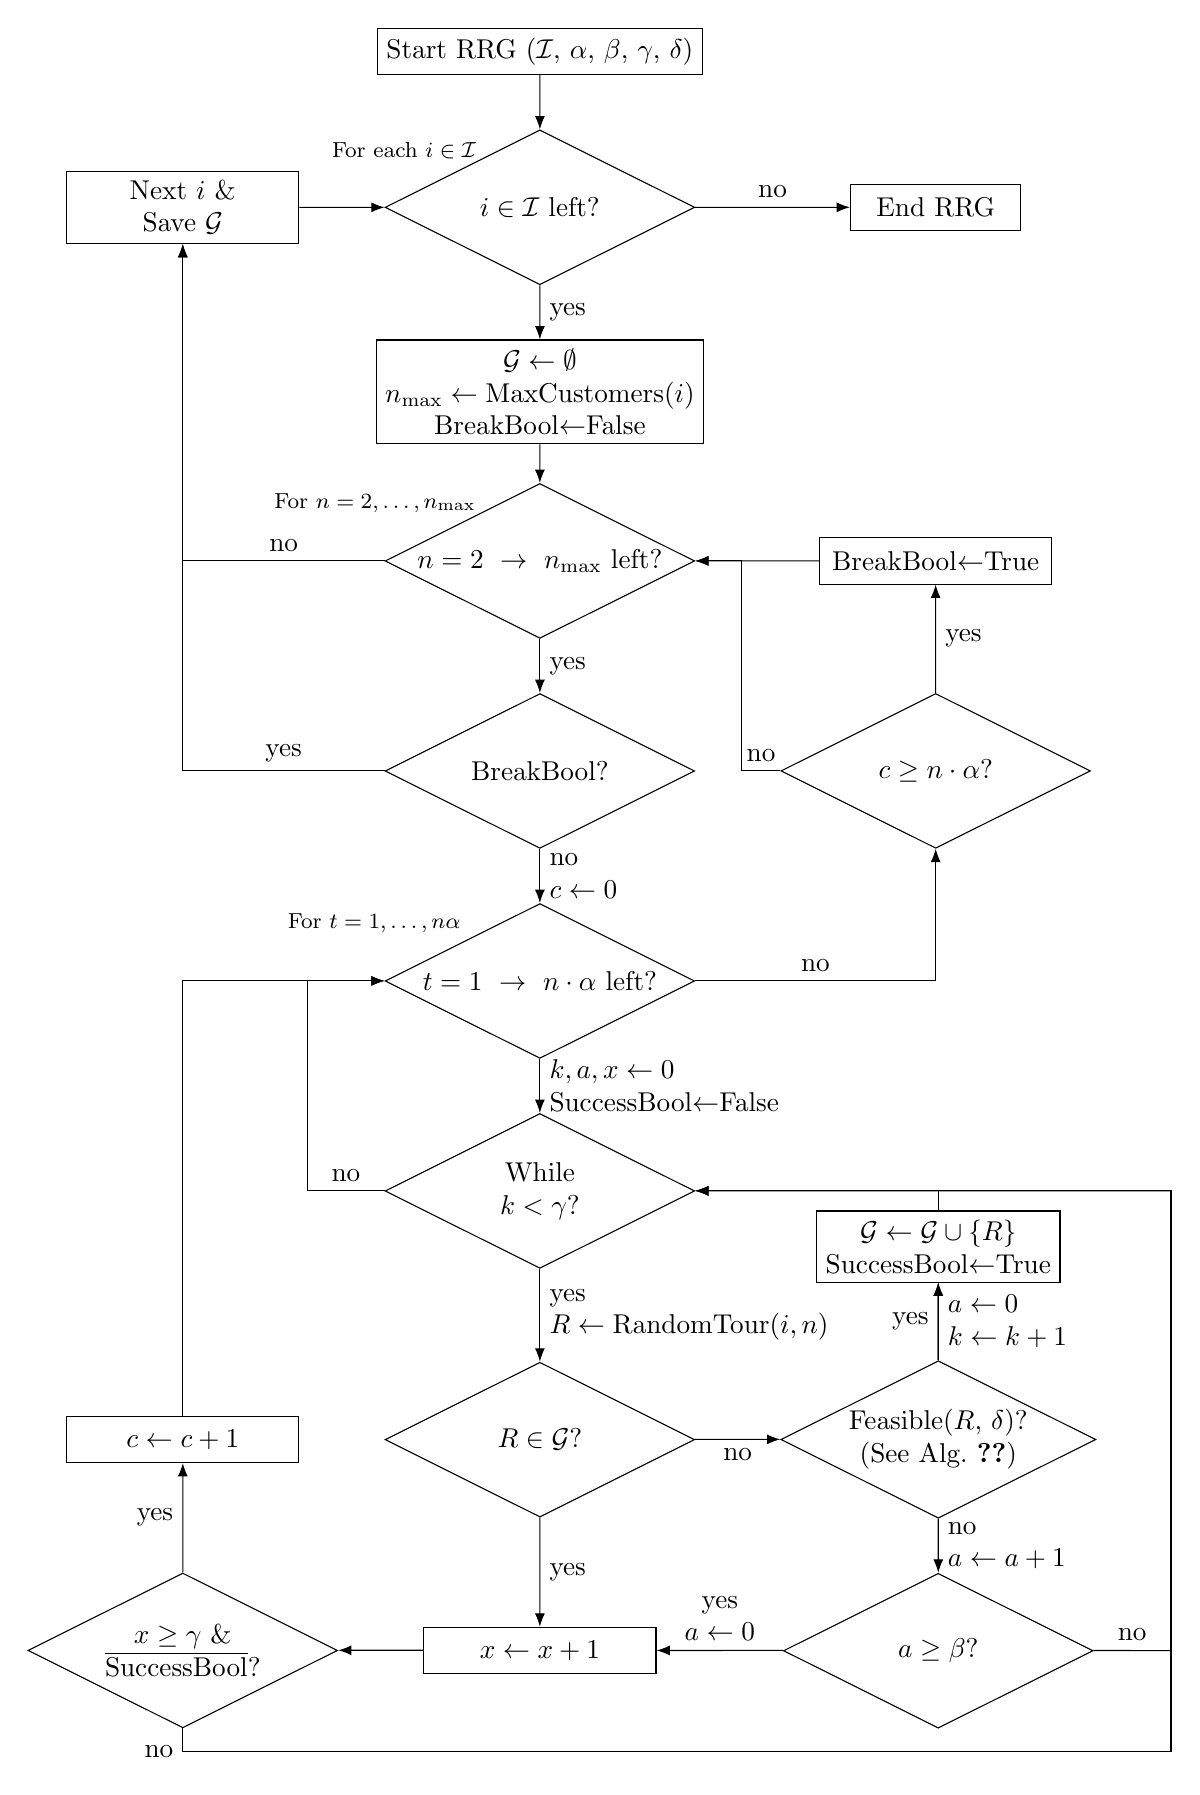
\begin{tikzpicture}[
            scale = 0.983, transform shape,node distance=7mm and 11mm,
            >=Latex,
            % Styles
            startstop/.style   = {rectangle, draw, align=center, minimum width=22mm, minimum height=6mm},
            process/.style     = {rectangle, draw, align=center, minimum width=30mm, minimum height=6mm},
            decision/.style    = {diamond, draw, aspect=2, inner sep=1pt, align=center, minimum width=40mm,minimum height=20mm},
            io/.style          = {trapezium, trapezium left angle=60, trapezium right angle=120, draw, align=center, minimum height=6mm},
            connector/.style   = {circle, draw, inner sep=1pt},
            line/.style        = {->}
        ]

        % Nodes
        \node[startstop] (start) {Start RRG ($\mathcal{I}$, $\alpha$, $\beta$, $\gamma$, $\delta$)};
        \node[decision, below=of start] (forI) {$i\in\mathcal{I}$ left?};
        \node[process, left= of forI] (nextI) {Next $i$ \&\\ Save $\mathcal{G}$};
        \node[process, below=of forI] (initI) {$\mathcal{G}\gets\emptyset$\\$n_{\max}\gets \mathrm{MaxCustomers}(i)$\\BreakBool$\gets$False};
        \node[decision, below=5mm of initI] (forN) {$n=2\ \to\ n_{\max}$ left?};
        \node[decision, below=of forN] (exitOuter) {BreakBool?};
        \node[decision, right=of exitOuter] (breakDec) {$c \geq n \cdot \alpha$?};
        \node[startstop] at ($(breakDec.north |- forI.east)$) (end) {End RRG};
        \node[decision, below=of exitOuter] (forAlpha) {$t=1\ \to\ n\cdot\alpha$ left?};
        \node[decision, below=of forAlpha] (whileK) {While\\$k<\gamma$?};
        \node[decision, below=12 mm of whileK] (dup) {$R\in\mathcal{G}$?};
        % \node[process, bel=of dup] (drawThresh) {$Q^*\gets Q\cdot \mathcal{U}_\delta^1$\\$V^*\gets V\cdot \mathcal{U}_\delta^1$};
        \node[decision, right=of dup] (feasible) {Feasible($R$, $\delta$)?\\(See Alg.~\ref{alg:appendix:check_single_tour})};
        \node[process, above=10mm of feasible] (accept) {$\mathcal{G}\gets \mathcal{G}\cup\{R\}$\\SuccessBool$\gets$True};
        \node[decision, below= of feasible] (attemptCond) {$a\ge \beta$?};
        \node[process] at ($(dup.south |- attemptCond.west)$) (incX) {$x\gets x+1$};
        \node[process, left=of dup] (incC) {$c\gets c+1$};
        \node[decision] at ($(incC.south |- incX.west)$)  (breakCond) {$x\ge \gamma$ \& \\$\overline{\text{SuccessBool}}$?};
        \node[process] at ($(breakDec.north |- forN.east)$) (trueExit) {BreakBool$\gets$True};

        % Edges
        \draw[line] (start) -- (forI);
        \draw[line] (forI) -- node[pos=0.5, right]{yes}(initI);
        \draw[line] (forI) -- node[pos=0.5, above]{no}(end);
        \draw[line] (initI) -- (forN);
        \draw[line] (nextI.east)-- (forI.west);
        \draw[line] (forAlpha.east) -| node[pos = 0.25,above]{no}(breakDec.south);
        \draw[line] (breakDec.west) -- node[pos = 0.5,above]{no}($(breakDec.west)-(5mm,0)$) |- (forN.east);
        \draw[line] (breakDec) -- node[pos = 0.5,right]{yes}(trueExit);
        \draw[line] (trueExit) -- (forN);
        \draw[line] (whileK.west) -- ($(whileK.west)-(10mm,0)$) coordinate (bend) node[pos = 0.5,above]{no} |- (forAlpha.west);

        \draw[line] (forN.south) --  node[pos=0.5, right]{yes}(exitOuter.north);
        \draw[line] (forN.west) -|  node[pos=0.25, above]{no}(nextI.south);
        \draw[line] (exitOuter.west) -| node[pos=0.25, above]{yes} (nextI.south);

        \draw[line] (exitOuter) -- node[pos=0.5, right, align=left]{no\\$c \gets 0$} (forAlpha);

        \draw[line] (forAlpha) -- node[pos=0.5, right, align=left]{$k,a,x\gets 0$\\ SuccessBool$\gets$False} (whileK);
        \draw[line] (whileK) --node[pos=0.5, right, align=left]{yes \\ $R\gets \mathrm{RandomTour}(i,n)$} (dup);
        \draw[line] (dup) -- node[pos=0.5, below]{no}(feasible);
        \draw[line] (dup) -- node[pos=0.5, right]{yes}(incX);
        \draw[line] (incX) -- (breakCond);
        %\draw[line] (breakCond) -- node[pos=0.25, below right]{no}(whileK);
        \draw[line] (breakCond) |- node[pos=0.5, left]{no}($(incX.south)-(0,10mm)$) -| ($(attemptCond.east)+(10mm,0)$) coordinate (bend)|- (whileK);
        \draw[line] (breakCond) -- node[pos=0.5, left]{yes} (incC);
        \draw[line] (incC) |- (forAlpha);

        \draw[line] (feasible) -- node[pos=0.5, left]{yes}(accept);
        \draw[line] (feasible) -- node[pos=0.5, right, align=left]{$a \gets 0$ \\ $k\gets k+1$}(accept);
        \draw[line] (accept.north) |- (whileK.east);

        \draw[line] (feasible) --node[pos=0.5, right, align=left]{no\\$a\gets a+1$} (attemptCond);
        \draw[line] (attemptCond) --node[pos=0.5, above, align=center]{yes\\$a\gets 0$} (incX);
        \draw[line] (attemptCond) -- ($(attemptCond.east)+(10mm,0)$) coordinate (bend) node[pos = 0.5,above]{no} |- (whileK);

        % Labels for the for-loops (optional, visual clarity)
        \node[above left=0mm and -3mm of forI] {\footnotesize For each $i\in\mathcal{I}$};
        \node[above left=0mm and -3mm of forN] {\footnotesize For $n=2,\dots,n_{\max}$};
        \node[above left=0mm and -1mm of forAlpha] {\footnotesize For $t=1,\dots,n\alpha$};

    \end{tikzpicture}
    \caption{Flowchart for Random Routes Generation (RRG).}
    \label{fig:flowchart_randomRouteGeneration}
\end{figure}

\section{Model Training}
\label{sec:ModelTraining}

\section{Features}
\label{sec:Features}

\chapter{Algorithm}
\label{chap:algorithm}
The focus for the algorithm was not to implement the best metaheuristic available for both routing and loading, but
to use a simple and adaptable algorithm and instead lays on how a trained classifier can
be integrated into exisiting \gls{3L-CVRP} algorithms and what are the impacts on the algorithm. Therefore the \gls{ILS}
algorithm was chosen, a moderate and simple algorithm used regularly for the \gls{VRP}. First, the principal
algorithm and the neighborhoods will be explained. Second, the emphasis is set on the feasibility check for the loading,
both which options are present and where to include it. Third, different strategies for the usage of the
classifier are presented.

\section{Principal Algorithm}
\label{sec:algorithm}
The \gls{ILS} algorithm was proposed by \cite{lourenco_iterated_2003} and has the goal to incorporate simplicity and generality.
As the authors say, metaheuristics became recently too sophisticated and problem specific and lack the purpose of
being applied to different use cases. The main concept is based on iterations of the metaheuristic, in which the current
solution is first perturbated (diversification) and afterwards improved by different sequential local search neighborhoods
(intensification). The solution process restarts with the best solution after a number of iterations without improvement
or continues with the current solution to explore new areas of the solution space.
The proposed base algorithm is depicted in Algorithm~\ref{alg:base_ILS}. Here, $s^*$ stands for the best solution, $s\sp{\prime}$
for a perturbated neighbor of $s^c$ and $s\sp{c}$ for the current solution. Note that the symbol $s^c$
is used as a placeholder, and shows the current state of the solution after each step. So the current solution
$s^c$ before the perturbation is usually different from $s^c$ after the local search, but, as the non-deterministic
perturbation and local search can return to the same solution, ambiguity exists to a certain extent.
It must be noted, that the constructive heuristic and  the neighborhoods for perturbation and local search need to be adapted to
each use case. The acceptance criterion can have several different implementations. To name a few, the algorithm could always
generate a random restart after a certain number of iterations without improvement, set back to the actual best solution
obtained or incorporating a \gls{SA} component accepting also worse solutions in the beginninng. The major challenge is
to find a fitting perturbation mechanism, which allows to explore new solution space areas, without falling back to previous solutions
after the local search. Therefore it should be guaranteed, that several iterations can be used for diversification and
intensification before resetting the algorithm. History is refered in the algorithm to some knowledge base,
to save the values of previos solution to skip already reached solutions or the iterations number without improvement since the
last restart or solution improvement.\footcite[cf.][]{lourenco_iterated_2003}
\begin{algorithm}[ht]
    \caption{General Iterated Local Search Algorithm}\label{alg:base_ILS}
    \begin{algorithmic}[1]
        \Procedure{ILS}{}
        \State $s_0 = \text{GenerateInitialSolution()}$
        \State $s^*,\,s^c = \text{LocalSearch}(s_0)$
        \While{$ \text{stop condition not met}$} \Comment{Total run time}
        \State $s'  = \text{Perturbation}(s^c, history)$
        \State $s\sp{c}  = \text{LocalSearch}(s\sp{\prime})$
        \State $s^c = \text{Acceptance Criterion}(s^*,\,s\sp{c}, history)$
        \EndWhile
        \State \textbf{return} $s^*$
        \EndProcedure
    \end{algorithmic}
\end{algorithm}

The presented base \gls{ILS} was adapted for this work to obtain good solutions for the \gls{3L-CVRP}, where for the \gls{VRP}
the overall costs need to be minimized, and every single tour needs to represent a feasible packing of the \gls{CLP}.
Therefore the following algorithm~\ref{alg:principal_ILS} was constructed. The perturbation applies $R$ random moves
to the current solution for each  neighborhood selected. In the \gls{LS}
the selected neighborhoods are sequentially walked through updating the current solution for each feasible improvement on
the current solution. The acceptance criterion controls the solution process updating the current solution, until a new overall
best solution was found or the limit for iterations without improvement (attempts limit $a$) is reached, then the current solution is resetted
to the best solution found. It needs to be investigated, if the random perturbation is able to leave local optima
when no improvements can be found or if this acceptance criterion is sufficient. But as the feasibility check of the loading
generated the key CPU time demand, the routing algorithm is kept simple. The \gls{ILS} has a dual stop criterion, existing on a maximum time limit for the metaheuristic and a maximum number of
iterations since the last improvement on the best solution was found. The second criterion needed to be added
to avoid exponential cycling of solutions, after the best solution was found.\footnote{Results compared with
    minimal costs due to \cite{tamke_branch-and-cut_2024}}

\begin{algorithm}[htb]
    \caption{Base Iterated Local Search Algorithm}\label{alg:base_ILS}
    \begin{algorithmic}[1]
        \Procedure{ILS}{$\text{AttemptsLimit}\,a,\, \text{RoundLimit}\,b$}
        \State $S_0 = ModifiedSavings()$ \Comment{After Zhang 2015}
        \State $S^c = LocalSearch(S_0)$
        \State $S^* = S^c $
        \State $NoImpr \leftarrow 0$
        \While{$ \text{stop condition not met}$}
        \If{$NoImpr > a \times b$}
        \State $S^c  = BigPerturbation(S^c )$ \Comment{Include all Perturbationneighborhoods}
        \Else
        \State $S^c  = Perturbation(S^c )$ \Comment{Include one Perturbationneighborhood}
        \EndIf
        \State $S^c  = LocalSearch(S^c )$
        \State{}
        \If{$S^c $ is better than $S^*$}
        \State $S^* \gets S^c $; $NoImpr \gets 0$
        \Else
        \State $NoImpr \gets NoImpr + 1$
        \EndIf
        \State{}
        \If{$NoImpr > a$}
        \State $S^c \gets S^* $; $NoImpr \gets 0$
        \EndIf
        \EndWhile
        \State \textbf{return} $S^*$
        \EndProcedure
    \end{algorithmic}
\end{algorithm}
\parbreak

In Chapter~\ref{chap:computational_study} a parameter study od the base \gls{ILS} is conducted to test different
levels for the attempts limit $a$, the random moves $R$ and the order of the \gls{LS} and perturbation neighborhoods.

\subsubsection{Constructive}
The initial solution is obtained by using the Savings Algorithm from \cite{clarke_scheduling_1964}. It is one of
most applied constructive algorithms for the \gls{VRP}, and is described by the following procedure. In the beginning
a single tour is created for every customer and the potential savings, when two customers are combined in one tour
($s_{ij} = d_{ij} - d_{0i} - d_{j0}$) are calculated.
Afterwards the tours are merged until no negative savings are available, and the
procedure terminates with $K$ tours. \footcite[cf.][]{clarke_scheduling_1964} However, this constructive algorithm needs to be adapted
as the minimum distance solution can exceed the maximum numbers of vehicles $K_{max}$ allowed per instance.
The modified savings approach was proposed by \cite{zhang_evolutionary_2015} to generate initial feasible solutions.
The modification is based on two steps, if the number of routes of the solution is exceeding the vehicle limit. First,
the merge procedure continues until $K = K_{max}$ or no feasible merges exist. Second, a repair procedure is invoked
by removing the routes with the least volume utilization from the solution and sorting the unassigned customers by
decreasing volume demand. Afterwards, the customers are tried to be reinserted at positions with the least
cost surplus. If no position could be found, the customer is inserted in a random chosen route by removing
other customers from this route to create free capacity. The second procedure is repeated until the
number of routes is $K = K_{max}$.\footcite[cf.][p.24]{zhang_evolutionary_2015}

\subsubsection{Neighborhoods}
\label{sec:neighborhoods}

The respected neighborhoods are divided in \textit{Intra}, changes on the customers within one tour, and \textit{Inter} neighborhoods,
changes between single tours. The following neighborhoods are implemented for each group:\footcite[cf.][pp. 89-90]{toth_vehicle_2014}

\begin{table}[ht]
    \centering
    \begin{tabular}{@{}P{0.3\textwidth}P{0.3\textwidth}@{}}
        \toprule
        \textbf{Intra} & \textbf{Inter} \\
        \midrule
        Swap           & Swap           \\
        Insertion      & Insertion      \\
        TwoOpt         &                \\
        \bottomrule
    \end{tabular}
\end{table}
Hereby, is a swap move defined by changing the position of two customers and insertion by removing one customer from one route
and replacing it in the same route (\textit{Intra}) or in another route (\textit{Inter}). A \textit{TwoOpt} move is characterized, when two arcs are deleted
from one route and are reinserted by swapping the indices of the arcs leading to a inversion of all customers between these two arcs.
For example, when the arcs $x_{12}$ are $x_{45}$ are selected the resulting arcs will be $x_{14}$ and $x_{25}$. To distinguish these
neighborhoods in the following section, they will be always called with their respective group, e.g. InterSwap. Additionally, a sixth
neighborhood is implemented deleting empty tours with no customers and is called \textit{DeleteEmptyRoutes}.

\parbreak

The neighborhoods for the perturbation are built upon the \textit{Inter} neighborhoods, and are characterized by $R$ random moves of
this respective neighborhood. Therefore they are called \textit{R\_InterInsertions} and \textit{R\_InterSwaps} in the
following. The perturbation neighborhood consists of inter neighborhoods as the diversification of the solution is
greater as with intra random moves. Regarding to \cite{lourenco_iterated_2003}, it is important, that perturbation holds the potential
to escape local optima and lays the foundation for a succesful \gls{LS}.\footcite[cf.][pp. 329f.]{lourenco_iterated_2003}

\section{Local Search and Perturbation}
\label{sec:LSandPerturbation}

In the \gls{LS} all selected neighborhoods are sequentially applied once. In the beginning all moves for the respective niehghborhood
are found, which lower the routing cost of the current solution. A move is defined by the modification of the current solution to
obtain a new solution. Note, that the loading is only respected with bound checks of the maximum volume and weight
allowed per container at this step.
Afterwards, all moves are sorted with decreasing savings and are applied to the current solution. Now, it is tested
if the new solution aligns to the three dimensional loading constraints. This feasibility check will be discussed in
detail in the next section. If the new route is feasible, the \gls{LS} restarts for this solution, if it is infeasible
the move will be reverted and the next move will be applied. If there are no moves with negative savings left to apply, the search
terminates and continues with the next neighborhood. The procedure is visualized in Figure~\ref{fig:LocalSearch} for one \gls{LS} neighborhood.
\begin{figure}[htbp]
    \centering
    {
        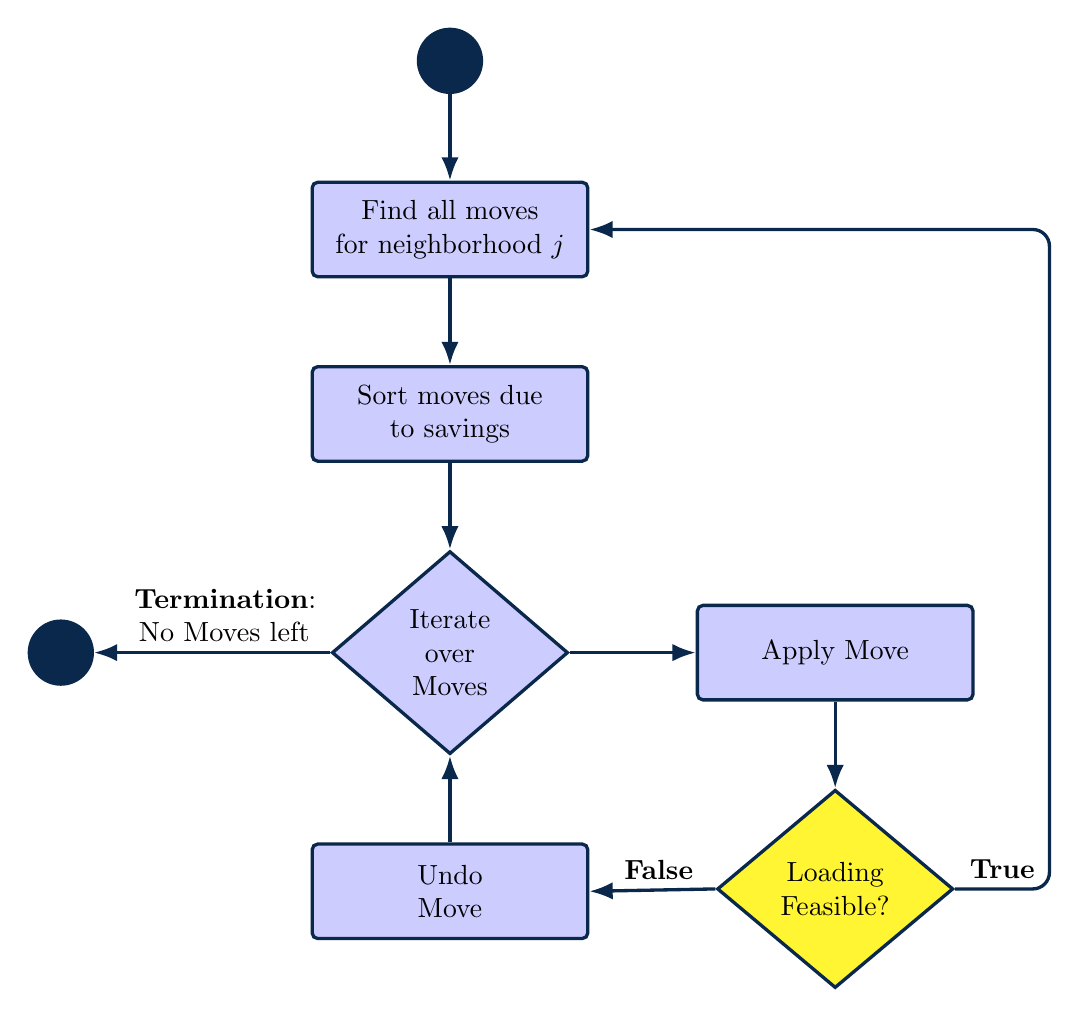
\begin{tikzpicture}[node distance=11mm and 16mm]
            % local defs for THIS picture only
            \begin{scope}
                % Nodes
                \node[dot] (start) {};
                \node[block, below=of start] (find) {Find all moves \\ for neighborhood $j$};
                \node[block, below=of find] (sort) {Sort moves due\\ to savings};
                \node[decision, below=of sort] (d1) {Iterate\\ over \\ Moves};
                \node[dot, left=30mm of d1] (leftdot) {};
                \node[block,  below=of d1] (undo)   {Undo\\ Move};
                \node[block,  right=of d1] (apply){Apply Move};
                \node[decisionY, below=of apply] (d2){Loading\\ Feasible?};

                % Arrows
                \draw[line] (start) -- (find);
                \draw[line] (find) -- (sort);
                \draw[line] (sort) -- (d1);
                \draw[line] (d1.west) -- node[pos=.45,above,text width=3cm,align=center]{\textbf{Termination}: No Moves left} (leftdot);
                \draw[line] (d1) -- (apply);
                \draw[line] (apply) -- (d2.north);
                \draw[line] (d2.west) -- node[pos =.45,above,align=center]{\textbf{False}} (undo.east);
                \draw[line] (undo.north) -- (d1.south);
                \coordinate (bump) at ($(d2.east)+(12mm,0)$); % how far to go right
                \draw[line]
                (d2.east) -- node[pos=0.5,above,align=center]{\textbf{True}}(bump)
                |- (find.east);

            \end{scope}
        \end{tikzpicture}
    }
    \caption{Local Search Procedure}
    \label{fig:LocalSearch}
\end{figure}


The perturbation has a similar approach, here in each neighborhood a certain number of random moves $R$ must be found
before the perturbation neighborhood terminates. The random move creation must not violate the maximum volume and weight limit of the vehicle.
The perturbation can be further be controlled by the number of neighborhoods being applied and the order of the neighborhoods.
Other perturbation mechanism like FourOpt or BlockInsertion were not considered as the Feasibility check of the loading is the limiting factor even though
the perturbation has bigger impact in creating new structural solutions.\footcite[cf.][pp. 329-332]{lourenco_iterated_2003}
The perturbation procedure is visualized in the following Figure~\ref{fig:Perturbation}.


\begin{figure}[htbp]
    \centering
    {
        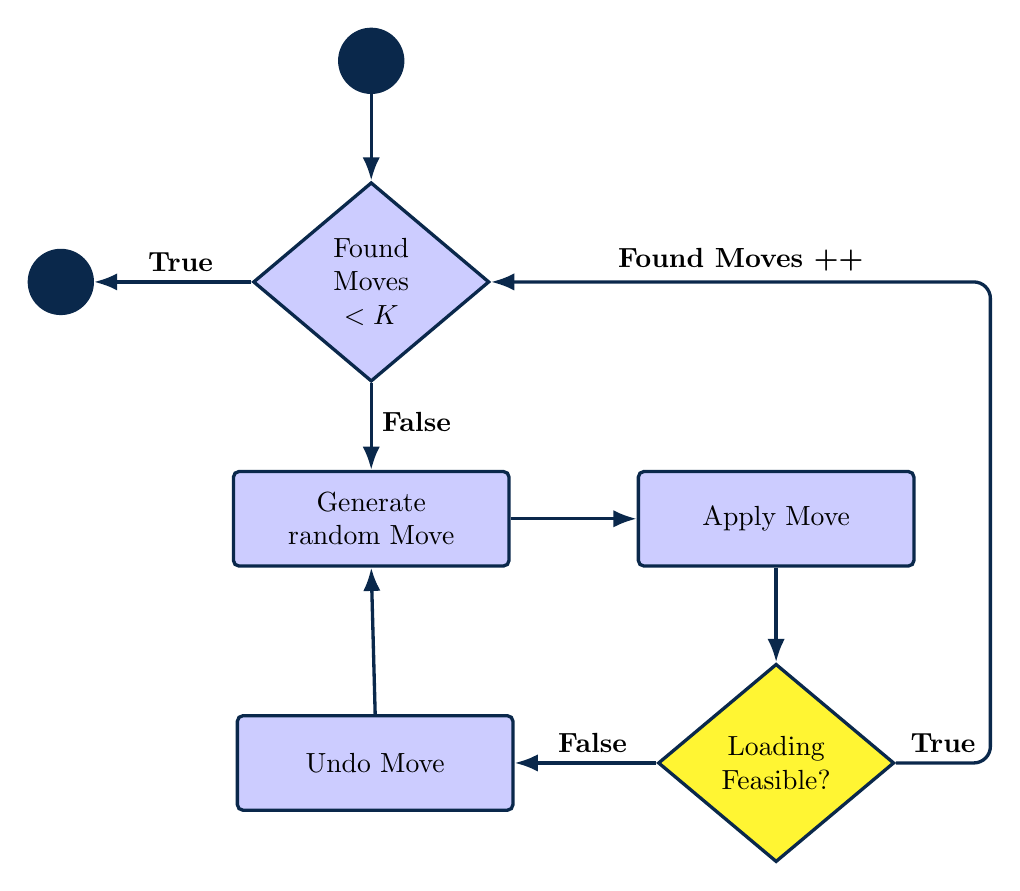
\begin{tikzpicture}[node distance=11mm and 16mm]
            % local defs for THIS picture only
            \begin{scope}
                % Nodes
                \node[dot] (start) {};
                \node[decision, below=of start] (d1) {Found\\ Moves \\ $< K$};
                \node[dot, left=20mm of d1] (leftdot) {};
                \node[block,  below=of d1] (gen)   {Generate\\ random Move};
                \node[block,  right=of gen] (apply){Apply Move};
                \node[decisionY, below=12mm of apply] (d2){Loading\\ Feasible?};
                \node[block,  below=of gen, left=18mm of d2] (undo) {Undo Move};

                % Arrows
                \draw[line] (start) -- (d1);
                \draw[line] (d1.west) -- node[pos=.45,above, align=center]{\textbf{True}} (leftdot);
                \draw[line] (d1.south) -- node[pos=.45,right,align=center]{\textbf{False}} (gen.north);
                \draw[line] (gen) -- (apply);
                \draw[line] (apply) -- (d2.north);
                \draw[line] (d2.west) -- node[pos =.45,above,align=center]{\textbf{False}} (undo.east);
                \draw[line] (undo.north) -- (gen.south);
                \coordinate (bump) at ($(d2.east)+(12mm,0)$); % how far to go right
                \draw[line]
                (d2.east) -- node[pos=0.5,above,align=center]{\textbf{True}}(bump)
                |- node[pos=.75,above,align=center]{\textbf{Found Moves ++}}
                (d1.east);

            \end{scope}
        \end{tikzpicture}
    }
    \caption{Perturbation Procedure}
    \label{fig:Perturbation}
\end{figure}


\section{Loading Feasibility Check}
\label{sec:FeasibilityCheck}
So far the description of the algorithm was reduced in minimizing the costs of the \gls{VRP} masterproblem and in vague
requirements, that new solutions need to be feasible regarding the three-dimensional loading constraints.
This check is time-consuming as every item need to placed accordingly in the container, testing all possible combinations.
The \gls{CLP} is $NP$-hard and as shown in Section~\ref{sec:classical_solution_approaches} most approaches rely on fast, but not
optimal heuristics. The aim of the thesis is to determine, if the usage of a binary classifier can bring quality and
speed advantages in comparison to the baseline of only using the exact solver.
As this work is a potential study, the combination with an exact solver is sufficient to derive insights for other use cases
leveraging either exact \gls{3L-CVRP} algorithms or exisiting metaheuristics with a classifier.
Before explaining how both tools can be integrated in the algorithm, strengths and weaknesses of
each approach are shown in the following overview:

\begin{figure}[ht]
    \centering
    \begin{minipage}[centering]{0.45\textwidth}
        \textbf{CP Solver}
        \begin{itemize}
            \item Returns exact loading status
            \item Computational heavy
            \item No need to verify solution
        \end{itemize}
    \end{minipage}
    \begin{minipage}[centering]{0.45\textwidth}
        \textbf{Binary Classifier}
        \begin{itemize}
            \item Fast to classify route
            \item Solution needs to be verified
            \item Adaptable acceptance threshold $y$
        \end{itemize}
    \end{minipage}
\end{figure}

The classifier has the potential to speed up the \gls{3L-CVRP} solution process, but accepted solutions need to be
verified with the \gls{CP} solver in a certain pattern to avoid false positive solutions during the algorithm.
Therefore the following four strategies are introduced, which determine how the loading feasibility can be checked and are
visualized in Figure~\ref{fig:tikz_four_variants}

\begin{figure}[ht]
    \centering
    % First row
    \begin{minipage}[t]{0.45\textwidth}
        \centering
        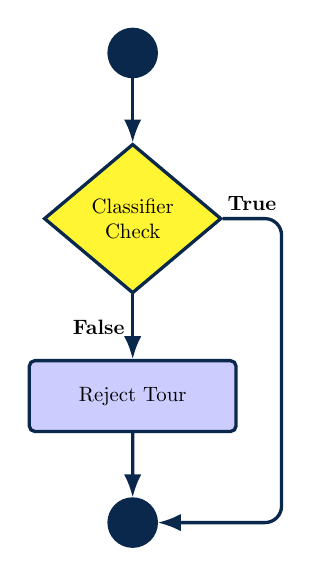
\begin{tikzpicture}[node distance=11mm and 16mm,scale=0.75, transform shape]
            \begin{scope}
                % Nodes
                \node[dot] (start) {};
                \node[decisionY, below=of start] (d1) {Classifier\\Check};
                \node[block,  below=of d1] (Reject){Reject Tour};
                \node[dot, below=of Reject] (end) {};
                % Arrows
                \draw[line] (start) -- (d1);
                \draw[line] (d1) -- node[pos=0.5,left]{\textbf{False}}(Reject);
                \draw[line] (Reject) -- (end);
                \coordinate (bump) at ($(d1.east)+(10mm,0)$); % how far to go right
                \draw[line]
                (d1.east) -- node[pos=0.5,above]{\textbf{True}}(bump)
                |- (end.east);
            \end{scope}
        \end{tikzpicture}
        \caption{SpeedUp Variant}
        \label{alg:tikz_variant1}
    \end{minipage}
    \hfill
    \begin{minipage}[t]{0.45\textwidth}
        \centering
        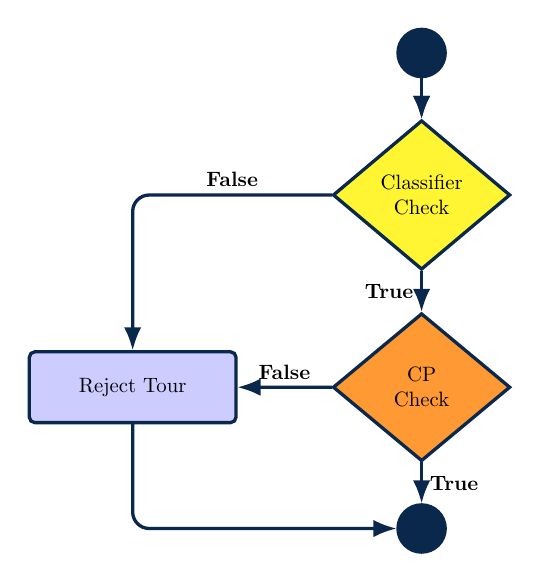
\begin{tikzpicture}[node distance=7mm and 16mm,scale=0.75, transform shape]
            \begin{scope}
                % Nodes
                \node[dot] (start) {};
                \node[decisionY, below=of start] (d1) {Classifier\\Check};
                \node[decisionCP, below=of d1] (d2) {CP\\Check};
                \node[block,  left=of d2] (Reject){Reject Tour};
                \node[dot, below=of d2] (end) {};
                % Arrows
                \draw[line] (start) -- (d1);
                \draw[line] (start) -- (d1);
                \draw[line] (d1) -- node[pos=0.5,left]{\textbf{True}}(d2);
                \draw[line] (d1) -| node[pos=0.25,above]{\textbf{False}}(Reject);
                \draw[line] (d2) -- node[pos=0.5,above]{\textbf{False}}(Reject);
                \draw[line] (d2) -- node[pos=0.5,right]{\textbf{True}}(end);
                \draw[line] (Reject) |- (end);
                \coordinate (bump) at ($(d1.east)+(10mm,0)$); % how far to go right
            \end{scope}
        \end{tikzpicture}
        \caption{Filter Variant}
        \label{alg:tikz_variant2}
    \end{minipage}

    \vspace{2em} % space between rows

    % Second row
    \begin{minipage}[t]{0.45\textwidth}
        \centering
        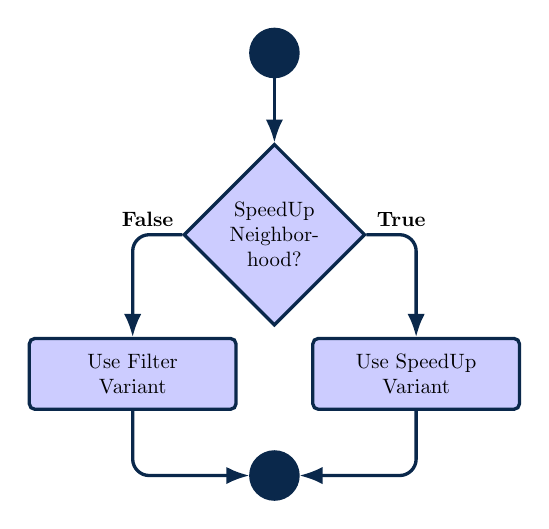
\begin{tikzpicture}[node distance=11mm and 0mm,scale=0.75, transform shape]
            \begin{scope}
                % Nodes
                \node[dot] (start) {};
                \node[decision, below=of start] (d1) {SpeedUp\\Neighbor-\\hood?};
                \coordinate (mid_up) at ($(d1.south)$);
                \node[block] at ($(mid_up)+(-24mm,-8mm)$) (Filter){Use Filter \\ Variant};
                \node[block] at ($(mid_up)+(24mm,-8mm)$)(SpeedUp){Use SpeedUp \\ Variant};
                % midpoint between the bottoms of Filter and SpeedUp
                \coordinate (mid) at ($(Filter.south)!0.5!(SpeedUp.south)$);

                % place the end dot some distance below that midpoint
                \node[dot] (end) at ($(mid)+(0,-11mm)$) {};
                % Arrows
                \draw[line] (start) -- (d1);
                \draw[line] (d1) -| node[pos=0.35,above]{\textbf{False}}(Filter);
                \draw[line] (d1) -| node[pos=0.35,above]{\textbf{True}}(SpeedUp);
                \draw[line] (Filter.south) |- (end.west);
                \draw[line] (SpeedUp.south) |- (end.east);
            \end{scope}
        \end{tikzpicture}
        \caption{Hybrid Variant}
        \label{alg:tikz_variant3}
    \end{minipage}
    \hfill
    \begin{minipage}[t]{0.45\textwidth}
        \centering
        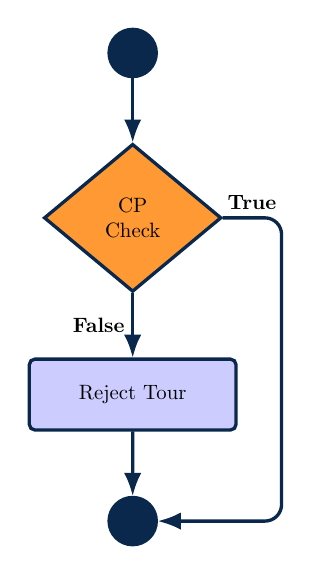
\begin{tikzpicture}[node distance=11mm and 16mm,scale=0.75, transform shape]
            \begin{scope}
                % Nodes
                \node[dot] (start) {};
                \node[decisionCP, below=of start] (d1) {CP\\Check};
                \node[block,  below=of d1] (Reject){Reject Tour};
                \node[dot, below=of Reject] (end) {};
                % Arrows
                \draw[line] (start) -- (d1);
                \draw[line] (d1) -- node[pos=0.5,left]{\textbf{False}}(Reject);
                \draw[line] (Reject) -- (end);
                \coordinate (bump) at ($(d1.east)+(10mm,0)$); % how far to go right
                \draw[line]
                (d1.east) -- node[pos=0.5,above]{\textbf{True}}(bump)
                |- (end.east);
            \end{scope}
        \end{tikzpicture}
        \caption{No Classifier Variant}
        \label{alg:tikz_variant4}
    \end{minipage}

    \caption{All schematic differences how feasibility is checked!}
    \label{fig:tikz_four_variants}
\end{figure}


The first approach is the \textit{SpeedUp} strategy, where only the classifier is used for feasibility checks during perturbation and
\gls{LS}. After $\omega$ /gls{ILS} iterations the current solution is verified with the exact \gls{CP} solver and is either rejected or accepted.
The amount of false positive labeled routes is here crucial, as the probability to reject the solution grows likewise. It needs
to be studied, how the parameter $\omega$ influences this procedure as the chance exist, that infeasible tours become feasible
again during several iterations without verification.
The second strategy is called \textit{Filter}, here classifier and \gls{CP} solver are called sequentially for every
feasibiliy check. The goal is to filter out infeasible routes before verifying them exactly to save time in the exact check.
All false negative labeled routes represent a potential solution quality loss, as those tours will never be considered to be accepted.
The third strategy is a hybrid form between the last two presented, where the chosen strategy, \textit{Filter} or \textit{SpeedUp},
is dependent on the neighborhood structure (Perturbation, Intra- and Interneighborhood). The last and fourth strategy is the benchmark
for the other strategies and here no classifier is used during the procedure. The goal is to beat this strategy with well tuned
variations of the first ones. These variations are further explained in the Figure~\ref{fig:four_variants} by highlighting, where
in the algorithm, which kind of feasibility check is applied. The $\clubsuit$ represents the usage of the \gls{CP} Solver and
$\bigstar$ the sole usage of the classifier (SpeedUp variant). The concatenation $\bigstar\clubsuit$ imply the usage of the Filter
variant and \(\clubsuit \backslash \bigstar\clubsuit\) if the \gls{CP} Solver or Filter is applied. \(\bigstar\backslash\clubsuit\)
indicates the Hybrid variant, and either the SpeedUp or the NoClassifier strategy is applied. In the initial \gls{LS} the same
feasibility check is applied as in the \gls{LS}.

\begin{figure}[ht]
    \centering

    % First row
    \begin{minipage}[t]{0.45\textwidth}
        \textbf{Variant 1: SpeedUp}\par\vspace{0.5ex}
        \begin{algorithmic}[1]
            \State {ModifiedSavings \(\clubsuit \backslash \bigstar\clubsuit\)}
            \While{not stop condition}
            \ClassifierState{Perturbation}
            \ClassifierState{LocalSearch}
            \EndWhile
        \end{algorithmic}
    \end{minipage}
    \hfill
    \begin{minipage}[t]{0.45\textwidth}
        \textbf{Variant 2: Filter}\par\vspace{0.5ex}
        \begin{algorithmic}[1]
            \BothState{ModifiedSavings}
            \While{not stop condition}
            \BothState{Perturbation}
            \BothState{LocalSearch}
            \EndWhile
        \end{algorithmic}
    \end{minipage}

    \vspace{2em} % space between rows

    % Second row
    \begin{minipage}[t]{0.45\textwidth}
        \textbf{Variant 3: Hybrid}\par\vspace{0.5ex}
        \begin{algorithmic}[1]
            \State {ModifiedSavings \(\clubsuit \backslash \bigstar\clubsuit\)}
            \While{not stop condition}
            \State {Perturbation \(\bigstar\backslash \clubsuit\)}
            \State {LocalSearch \(\bigstar\backslash \clubsuit\)}
            \EndWhile
        \end{algorithmic}
    \end{minipage}
    \hfill
    \begin{minipage}[t]{0.45\textwidth}
        \textbf{Variant 4: NoClassifier}\par\vspace{0.5ex}
        \begin{algorithmic}[1]
            \CPState{ModifiedSavings}
            \While{not stop condition}
            \CPState{Perturbation}
            \CPState{LocalSearch}
            \EndWhile
        \end{algorithmic}
    \end{minipage}

    \vspace{1em}

    \caption[Four algorithm .]{Four variants to implement the classifier in the loading feasibility check ($\bigstar$
        does imply usage of classifier and $\clubsuit$ of the CP Solver).}
    \label{fig:four_variants}
\end{figure}


During the construction the \textit{SpeedUp} strategy can hardly be applied, which has two reasons. Firstly, this strategy relies
on rejecting solutions feasible with the classifier by the \gls{CP} Solver and resetting the solution to previous feasible solutions.
Secondly, the procedure of the modified savings algorihm is deterministic and repetitions will lead to the same solutions. In these
cases it needs to be investigated, if the \textit{Filter} strategy can speed up the solution process in the constructive without
great solution quality losses.

\parbreak

In the next chapter for each strategy a computational study will be conducted to compare them. To facilitate this approach,
a comparison of various published \gls{3L-CVRP} datasets will be conducted to compare and identify the most appropriate
dataset for training a binary feasibility classifier.

\subsection*{Parking Lot}
As discussed in Chapter~\ref{sec:classical_solution_approaches}, the verification of
packing feasibility for each individual route is computationally expensive.
Here, classifiers can significantly boost performance of existing exact algorithms by rapidly predicting the feasibility of the route. The
exact packing solution is then only computed for the final solution candidates or before an infeasible classified solution
is discarded to avoid incorrect eliminations, as presented above.

\chapter{Computational study}
\label{chap:computational_study}
This chapter will give the most insights into the functionality and efficiency of the usage of the presented binary classifier in
\gls{3L-CVRP} algorithms. This chapter will begin with the selection of two different suiting \gls{3L-CVRP} datasets by comparing
several datasets and presenting the most important specialities. Afterwards the results from training the model are presented, which
is divided in three main parts, firstly the results of the retrieval of the data, secondly the feature selection, and finally presenting
different strategies for comparing different models and selecting the best regarding accuracy on the test dataset as well as on collected
tensor data. Afterwards a parameter study is conducted for the \gls{ILS}, starting with the \textit{NoClassifier} variant determining
the best configurations for the base parameters, followed by a more intense comparisons of all the classifier parameters determining the
other three variants. This chapter closes with a complete comparison of all four variants, comparing the version with tuned parameters.
These insights lay the foundation for the following closing Chapter~\ref{chap:conclusion}.

\section{Comparison of Available Datasets}
\label{sec:dataset_selection}

The \gls{3L-CVRP} is a well-studied problem and several datasets were published in the past, considering
different constraints and characteristics. A selection of these datasets will be compared and evaluated
in this section. The goal is to identify a suitable dataset for training a general \gls{CLP} classifier that can predict
the feasibility of the \gls{CLP} of single tours from different datasets. Therefore, the dataset needs
heterogeneous characterists to represent numerous possible use-cases
as shown in Chapter~\ref{sec:motivation_feasibility_prediction}. Five published
\cgls{3L-CVRP} datasets are presented with respect to their overall characteristics.
Each dataset gets an unique identfier to simplify the comparison and is shown in parenthesis
after the following individual introduction. The first \cgls{3L-CVRP} dataset was published by \citeauthor{gendreau_tabu_2006} in
\citeyear{gendreau_tabu_2006} and delivered the first \cgls{3L-CVRP} instances containing huge and heavy items (\gendreauDataSet).\footcite[cf.][]{gendreau_tabu_2006}
The second dataset was published by \citeauthor{moura_integrated_2009} in \citeyear{moura_integrated_2009},
and combines the \gls{VRP} from \citeauthor{solomon_algorithms_1987} and the \gls{CLP} instances from
\citeauthor{bischoff_issues_1995} defining the \gls{3L-VRPTW} considering
many items of small size and weight (\mouraDataSet).\footcites[cf.][]{solomon_algorithms_1987,bischoff_issues_1995}[][]{moura_integrated_2009}
The first dataset containing real-life data was published by \citeauthor{ceschia_local_2013} in \citeyear{ceschia_local_2013}
and contains the instances with the most items (\ceschiaDataSet).\footcite[cf.][]{ceschia_local_2013}
Krebs published two different datasets in
\citeyear{krebs_advanced_2021} with a focus on more realistic constraints. The first one contains a set
of realistic constraints and offers a wide range of instance sizes (\krebsADataSet).\footcite[cf.][]{krebs_advanced_2021}
The second one focuses on semi-trailer trucks and special requirements for axle weights (\krebsBDataSet).\footcite[cf.][]{krebs_axle_2021}
The characteristics of the datasets are summarized in the following Table~\ref{tab:dataset_comparison},
where the brackets [\,] indicate a range of possible values. All values considering mass and volume are
\textit{relative} to the respective vehicle weight and volume limit to be comparable. A \textit{item type} is
defined by its geometrical dimensions, the weight, and possible stability characteristics, such as fragility or \gls{LBS}.
When the number of item types is smaller than the number of items, items with equal type occur multiple times. The item types
depict the number of different item types per instance. Additionaly
most features of the dataset are compared with \textit{aggregated}  values, referring to the aggregrated characteristics
of all items requested by one customer, so the aggregated mass, volume and items shows the value what is requested by an
average customer of this dataset.

\newcolumntype{C}[1]{>{\centering\arraybackslash}p{#1}}
\newcolumntype{L}[1]{>{\raggedright\arraybackslash}p{#1}} % left-aligned
\begin{table}[ht]
    \centering
    \small
    \renewcommand{\arraystretch}{1.1}   % a touch more row height
    \begin{tabular}{@{}lccccc@{}}
        \toprule
        \textbf{Dataset} & \textbf{Instances} & \textbf{Customers} & \textbf{Agg. Mass}\footnote{Average is based on all customers of the instances.} & \textbf{Agg. Vol.} \footnotemark[\value{footnote}]       & \textbf{Agg. Items}\footnotemark[\value{footnote}] \\
        \midrule
        \gendreauDataSet & 27                 & [15, 100]          & 0.137                                                                            & 0.127                                                    & 2.00                                               \\
        \mouraDataSet    & 46                 & 25                 & 0.077                                                                            & 0.176                                                    & 52.0                                               \\
        \ceschiaDataSet  & 13                 & [11, 129]          & 0.063                                                                            & 0.160                                                    & 18.1                                               \\
        \krebsADataSet   & 600                & [20, 100]          & 0.098                                                                            & 0.100                                                    & 4.41                                               \\
        \krebsBDataSet   & 80                 & [30, 120]          & 0.036                                                                            & 0.052                                                    & 4.00                                               \\
        \toprule
        \textbf{Dataset} & \textbf{Items}     & \textbf{Types}     & \textbf{\text{Routes}}\footnote{Average is based on the instances.}              & \textbf{\text{Route Len}}\footnotemark[\value{footnote}] & \textbf{Fragility}\footnotemark[\value{footnote}]  \\
        \midrule
        \gendreauDataSet & [26, 199]          & [26, 199]          & 6.13                                                                             & 6.22                                                     & 0.25                                               \\
        \mouraDataSet    & 1050, 1550         & 5                  & 4.40                                                                             & 6.72                                                     & 0.29                                               \\
        \ceschiaDataSet  & [254, 8060]        & [9, 97]            & 10.2                                                                             & 5.81                                                     & 0.10                                               \\
        \krebsADataSet   & 200, 400           & 3, 10, 100         & 6.77                                                                             & 13.6                                                     & 0.24                                               \\
        \krebsBDataSet   & 200, 400           & 10, 100            & 3.87                                                                             & 22.1                                                     & 0.10                                               \\
        \bottomrule
    \end{tabular}
    \caption[Numerical comparison of different 3L--CVRP Datasets.]{Numeric comparisons between five avalaible datasets.}
    \label{tab:dataset_comparison}
\end{table}

The values routes, route length and fragility show the average over all instances, and
routes define the \gls{LB} for needed vehicles and route lenght the \gls{UB} for the customers in a route based on the average
requested relative volume and mass. The averages are displayed to become a better understanding of the average
statistics of each dataset, rather than looking at extreme values.
The most important consideration, when selecting a suitable dataset for the training of a classifier,
is how representative single tours from one dataset are for all other datasets. Therefore, the numeric characteristics
should not contain outliers. It is apparent, that the \gendreauDataSetText dataset has the least items per customer
with huge relative volume and weight values, which leads with an average route length of 6.22 customers to very few items
considered per route in comparison to the other datasets. This makes it easier to compute the feasibility of the laoding
as the number of placing patterns is limited. The \mouraDataSetText has the most items per average per customer consisting
of only 5 item types. The \ceschiaDataSetText dataset contains the fewest instances, but with the most maximum items of 8060,
which lead to many routes on avrage with average length and many items per loading. The two datasets from Krebs, have similar
boundaries and values, but \krebsBDataSetText has routes with twice as many customers as \krebsADataSetText on average due
to the smaller average aggregated mass and volume requested by each customer. Both \krebsADataSetText and \gendreauDataSetText
show a good variety of the features, without including too many items per route in comparison to the other datasets.
The following Table~\ref{tab:constraint_matrix} provides an overview of the constraints considered
in each dataset showcasing the realistic profile. The constraints are categorized in the five groups introduced
in Section~\ref{sec:clp_definition}.
\clearpage

\begin{table}[ht]
    \centering
    \small
    \renewcommand{\arraystretch}{1.2}
    \begin{tabular}{@{}L{1.8cm}L{3cm}C{1.6cm}C{1.6cm}C{1.6cm}C{1.6cm}C{1.6cm}@{}}
        \toprule
        \textbf{Category}          & \textbf{Constraint} &                        &                     & \textbf{Dataset}      &                      &                      \\
                                   &                     & Gendreau\newline(2006) & Moura\newline(2009) & Ceschia\newline(2013) & Krebs\newline(2021a) & Krebs\newline(2021b) \\
        \midrule
        \multirow{3}{*}{Container} & Load Capacity       & $\bullet$              & $\bullet$           & $\bullet$             & $\bullet$            & $\bullet$            \\
                                   & Load Balance        &                        &                     &                       & $\bullet$            &                      \\
                                   & Axle Weights        &                        &                     &                       & $\bullet$            & $\bullet$            \\\midrule
        \multirow{3}{*}{Item}      & z-Rotation          & $\bullet$              & $\bullet$           & $\bullet$             & $\bullet$            & $\bullet$            \\
                                   & Fragility           & $\bullet$              &                     & $\bullet$             & $\bullet$            & $\bullet$            \\
                                   & LBS                 &                        &                     & $\bullet$             & $\bullet$            &                      \\\midrule
        \multirow{1}{*}{Cargo}     & Complete Shipm.     & $\bullet$              & $\bullet$           &                       & $\bullet$            & $\bullet$            \\\midrule
        \multirow{6}{*}{Position}  & Geometry            & $\bullet$              & $\bullet$           & $\bullet$             & $\bullet$            & $\bullet$            \\
                                   & Orthogonality       & $\bullet$              & $\bullet$           & $\bullet$             & $\bullet$            & $\bullet$            \\
                                   & Reachability        &                        &                     & $\bullet$             & $\bullet$            &                      \\
                                   & Sequence            & $\bullet$              &                     &                       & $\bullet$            &                      \\
                                   & LIFO                & $\bullet$              & $\bullet$           & $\bullet$             & $\bullet$            & $\bullet$            \\
                                   & MLIFO               &                        &                     & $\bullet$             & $\bullet$            &                      \\\midrule
        \multirow{2}{*}{Load}      & Robust Stability    &                        &                     & $\bullet$             & $\bullet$            &                      \\
                                   & Support Area        & $\bullet$              & $\bullet$           &                       &                      & $\bullet$            \\

        \bottomrule
    \end{tabular}
    \caption[Overview of CLP constraints in selected 3L--CVRP datasets.]{Matrix overview of constraints covered in selected datasets. A bullet ($\bullet$) indicates that the constraint is considered.}
    \label{tab:constraint_matrix}
\end{table}

This comparison shows that all datasets include similar types of constraints, but the level
of complexity varies. \krebsADataSetText and \ceschiaDataSetText stand out by incorporating
more advanced constraints such as robust stability, reachability, and \gls{LBS}, in comparison to
basic ones like support area, \gls{LIFO} and fragility. To further investigate the differences
between the datasets, Figure~\ref{fig:dataset_comparison} visualizes the aggregated relative mass and
volume of all items requested by individual customers.
Additionally, the size of each scatter point indicates the total number of items requested.
For example, the \mouraDataSetText dataset includes 46
instances with 25 customers each, resulting in $25 \cdot 46 = 1150$ dots in the plot.

\begin{figure}[ht]
    \centering
    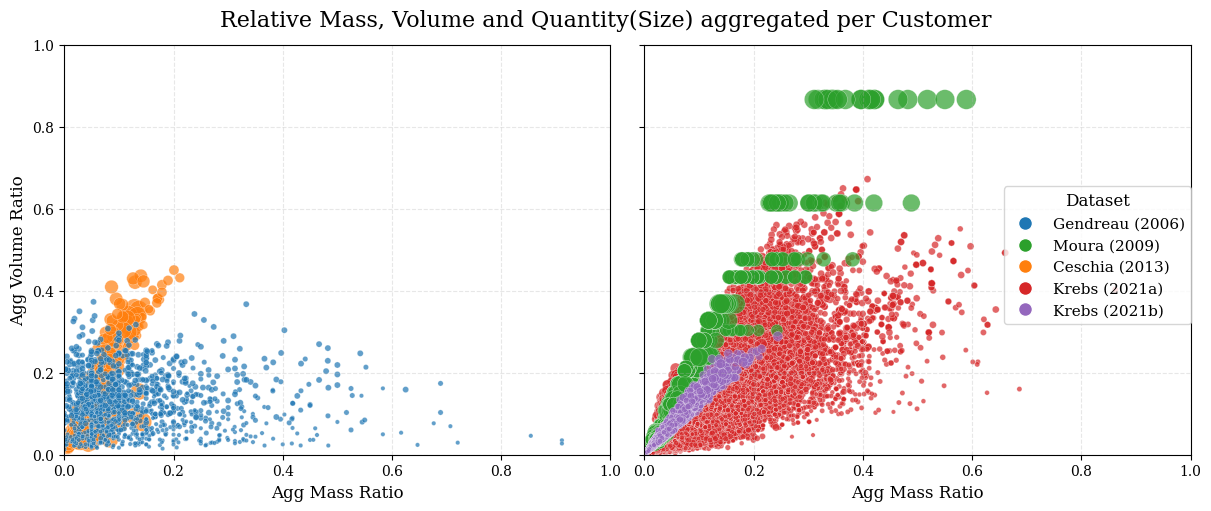
\includegraphics[width=0.85\textwidth]{pictures/comparison_datasets_3lcvrp.png}
    \caption{Comparison aggregated customer demands of different 3L--CVRP/ 3L--VRPTW datasets.}
    \label{fig:dataset_comparison}
\end{figure}

The dispersion of the data points reflects the diversity of individual instances in terms of volume
and mass dependency. A more balanced profile suggests that some customers tend to order items that
are either mass- or volume-intensive, which supports training the model on more heterogeneous data.
Therefore, the dataset should cover a wide range of cases, varying in mass, volume, and item
quantity per customer. The widest spread is observed in \krebsADataSetText and \gendreauDataSetText serving
both as good dataset candidates for training a classifier. Both datasets are investigated further in
the next section.

\section{Analsis of datasets}
\label{sec:analysis_datasets}

The two datasets, \krebsADataSetText and \gendreauDataSetText, have a good diverse profile for training
a binary classifier and to be further analyzed. It must be noted, that it is very likely more complex
to solve instances from the \krebsADataSetText as the number of customers in a route and the
aggregated number of items is on average twice as high as from \gendreauDataSetText (see Table~\ref{tab:dataset_comparison}).
As shown in Section~\ref{sec:literature_overview} several publications solved the Gendreau instance set
with various heuristics and even exact approaches, whereas only one heuristic solution approach exists for the instances of Krebs.
Both datasets are further analysed in this section to understand dataset specific properties, which could not
be shown in the previous section.

\subsubsection{\krebsADataSetText}

The dataset contains 18 different instance types resulting from the combinations
of number of customers, item types and items. The following Figure~\ref{fig:krebs_dataset_analysis_detailes} plots
the relative mass and volume of all items requested by individual customers for each of the 18 instances. Every color
represents one instance and the plots are divided by the number of respective customers in threee groups, presenting
6 combinations each. There are three levels for the different item types per [3,10,100] and two levels for the total
number of items, 200 and 400, per instance.

\begin{figure}[ht]
    \centering
    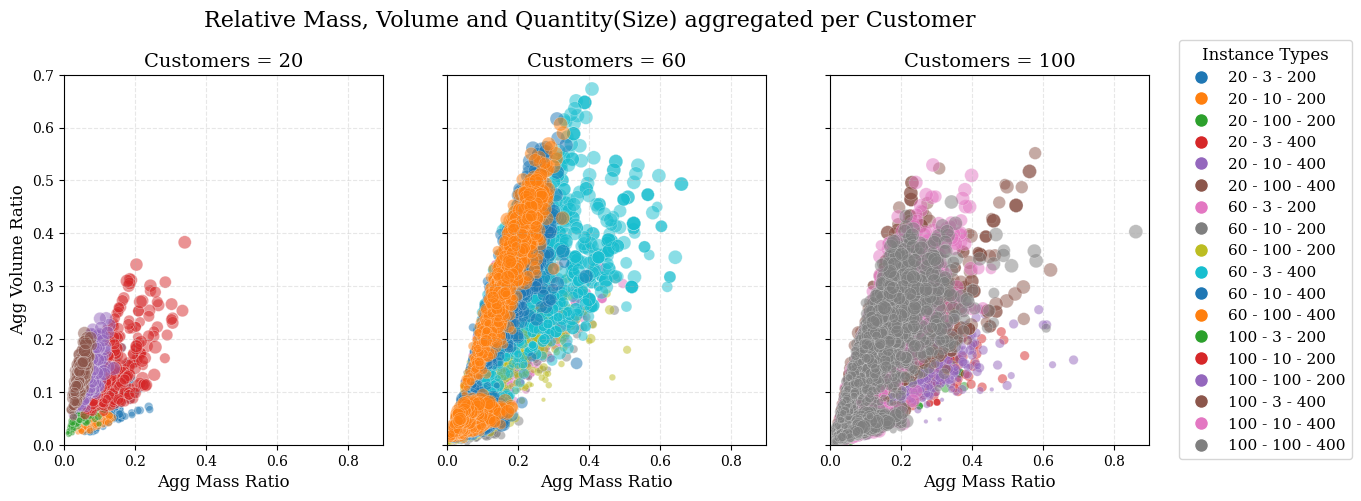
\includegraphics[width=0.85\textwidth]{pictures/krebs_instances_detailed.png}
    \caption[Visualization of different instances of \textcite{krebs_advanced_2021} dataset.]{Visualization of different instances of \krebsADataSetText dataset.
        The instances are named by the number of customers, item types and items.}
    \label{fig:krebs_dataset_analysis_detailes}
\end{figure}

Several insights can be obtained from the analysis of this plot. Firstly, the aggregated relative
volume and mass per customer is significantly lower for the 20 customers group than for the groups with 60 or 100 customers.
Secondly, the distribution differs from each instance type, ranging from quite linear distributions in a narrow
interval (e.g. instance 60-100-400) to quite broad distributions (e.g. instance 100-100-400). These two observations need to be considered,
when selecting instances to generate training data for the classifier to avoid a homogenous training set, and
as a consequence poor classifying results with a low accuracy. The instance set should be drawn from every group equally and
different distributions need to be considered per group, that the average route numeric route structure differs.

\subsubsection{\gendreauDataSetText}

This dataset consists of 27 instances, where the dispersion of the aggregated mass per customer is reaching very high values, up to
0.91, but has modest volume levels, with a maximum of 0.4 approximately, as could be seen in Figure~\ref{fig:dataset_comparison}. The
following Figure~\ref{fig:aggregated_gendreau_plots} show this dispersion per instance revealing an important insight about the dataset.
As the relative volume is quite for all instances, the relative mass differs between the instances. As it was analyzed from \cite{tamke_branch-and-cut_2024}
the complexity to solve the instances is far greater, when the items are more lightweight and the volume is the limiting factor
for packing items in the container. Furthermore, the authors distinguished the instances in a group of heavy items ($\mathcal{H}$) and
a group of lighweight items ($\mathcal{L}$) by dividing the two groups by the average weight utilization $\overline{\omega}$ of the found
groups. If $\overline{\omega} \geq 0.7$ then an instance belongs to $\mathcal{H}$ and for values smaller than 0.7 to $\mathcal{L}$.\footcite[cf.][pp. 23-25]{tamke_branch-and-cut_2024}
The obtained resutls for the Gendreau instances will be also differentiated in those two groups to investigate the effect of
the average weight utilization $\overline{\omega}$ on the solution quality and process.

\begin{figure}[ht]
    \centering
    \begin{tikzpicture}[node distance=0mm and 0mm]
        \node[anchor=south, inner sep=0] (A) at (0,0)
        {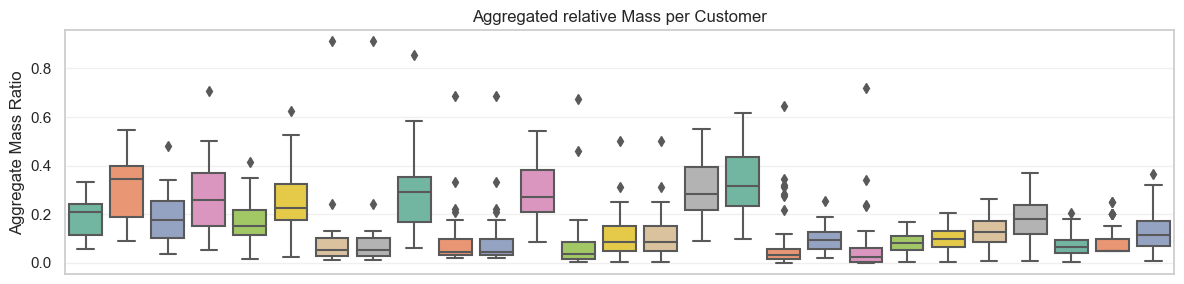
\includegraphics[width=0.95\textwidth]{pictures/AggMassCustGendreau.png}};
        \node[anchor=north, below=of A,inner sep=0] (B)
        {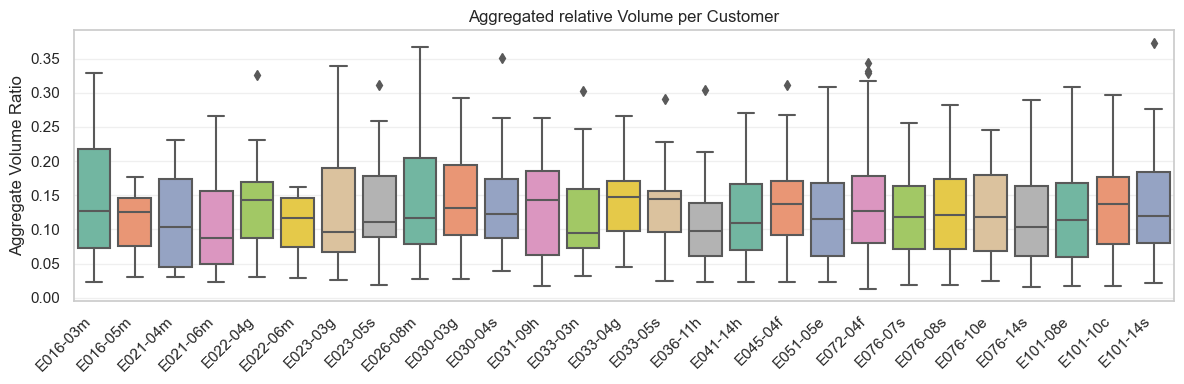
\includegraphics[width=0.96\textwidth]{pictures/AggVolCustGendreau.png}};
    \end{tikzpicture}
    \caption{Aggregated relative mass and volume per customer distributed for each instance of the \gendreauDataSetText dataset.}
    \label{fig:aggregated_gendreau_plots}
\end{figure}

In the following section the results from training the binary classifier are presented with diffferent datasets.

\section{Results Training}
\label{sec:ResultsTraining}

\subsection{Random Dataset Generation}
With the algorithm \ref{alg:rand_routes_generation} the following random datasets were created with all
instances from Gendreau.
\begin{table}[h!]
    \centering
    \begin{tabular}{c c cc c c c}
        \hline
        Multiplier $\alpha$ & Attempts limit $\beta$ & Success threshold $\gamma$ & Routes & Accuracy & F1-Score \\
        \hline
        2                   & 20                     & 20                         & 45733  &          &          \\
        2                   & 20                     & 30                         & 70067  &          &          \\
        2                   & 30                     & 20                         & 47350  &          &          \\
        2                   & 30                     & 30                         & 72408  &          &          \\
        3                   & 20                     & 20                         & 68506  &          &          \\
        3                   & 20                     & 30                         & 104967 &          &          \\
        3                   & 30                     & 20                         & 70843  &          &          \\
        3                   & 30                     & 30                         & 108597 &          &          \\
        4                   & 20                     & 20                         & 91000  &          &          \\
        4                   & 20                     & 30                         & 139996 &          &          \\
        4                   & 30                     & 20                         & 94666  &          &          \\
        4                   & 30                     & 30                         & 144311 &          &          \\
        5                   & 40                     & 40                         & 249762 &          &          \\
        \hline
    \end{tabular}
    \caption{Created instances for different parameter combinations $(X, Y, Z)$}
    \label{tab:created_instances_gendreau}
\end{table}

With a subset from krebs the following datasets were created!
\begin{table}[h!]
    \centering
    \begin{tabular}{c c cc c c c}
        \hline
        Multiplier $\alpha$ & Attempts limit $\beta$ & Success threshold $\gamma$ & Routes & Accuracy & F1-Score \\
        \hline
        1                   & 1                      & 1                          & 7616   &          &          \\
        1                   & 1                      & 2                          & 15948  &          &          \\
        1                   & 1                      & 3                          & 24573  &          &          \\
        1                   & 2                      & 1                          & 8325   &          &          \\
        1                   & 2                      & 2                          & 17217  &          &          \\
        1                   & 2                      & 3                          & 26467  &          &          \\
        1                   & 3                      & 1                          & 8683   &          &          \\
        1                   & 3                      & 2                          & 18041  &          &          \\
        1                   & 3                      & 3                          & 27535  &          &          \\
        \hline
    \end{tabular}
    \caption{Created instances for different parameter combinations $(X, Y, Z)$}
    \label{tab:created_instances_xyz}
\end{table}


\chapter{Conclusion and Outlook}
\label{sec:conclusion}
\begin{comment}
The variety of \gls{CLP} applications in logistics is wide, and the urge to consider practical constraints
and realistic datasets is high. For practitioners, heuristics are the first choice as good solutions
can be retrieved in satisfactory time. Exact solutions help to understand the structure of optimal solutions
and to evalutate and enhance existing heuristics. To accelerate exact methods different \gls{ML} enhancements
were presented and the \gls{3L-CVRP} was identified as a promising future use case for \gls{ML} classifiers.
The importance of realistic constraints of the \gls{CLP} were higlighted and the challenges faced when
training the classifier with such constraints were discussed. A dataset from \textcite{krebs_advanced_2021} was identified
was selected for future training of a classifier. To train a \gls{3L-CVRP} classifier that incorporates practical constraints, several next steps are
required. First, a training dataset must be created, consisting of individual tours that are pre-labeled
as feasible or infeasible using an exact \gls{CP} approach. In subsequent training iterations and epochs,
relevant features for accurately predicting feasibility must be evaluated. This includes assessing how
challenging it is to encode each individual constraint as a feature. Once the classifier achieves a
satisfactory level of accuracy, it can be integrated into a complete \gls{3L-CVRP} algorithm. The
classifier will then be used to predict the feasibility of solutions, enabling a comparison between
algorithmic performance with and without the classifier. Finally, the model can be tested on additional
problem instances—such as those introduced in Chapter 5—to evaluate its generalization capabilities.
This will allow the creation of meaningful benchmarks across multiple datasets.
% New start
The wide range of \gls{CLP} applications in logistics underscores the growing need to incorporate practical
constraints and realistic datasets. While heuristics remain the preferred choice for practitioners due to
their efficiency in producing good solutions within acceptable time frames, exact methods play a crucial
role in understanding the structure of optimal solutions and benchmarking heuristics.
To enhance exact solution approaches, two \gls{ML}-based examples have been presented, and the potential of
including classifiers in the solution process has been discussed. Main take aways are, that the training dataset
needs to be carefully selected including features, which can display the complex realistics \gls{CLP} constraints,
and representative data points, which are used also in the algorihtm the classifier is integrated into.
The \gls{3L-CVRP} has been identified as a promising candidate for the application of \gls{ML} classifiers,
as many tours need to be checked for packing feasibility and realistic constraints are needed to consider
practical logistical scenarios. The dataset from \textcite{krebs_advanced_2021} was
identified as a suitable foundation for future work training a classifier.
The next steps involve creating a labeled training dataset by creating \gls{VRP} tours, which are retrieved
by solving the \gls{3L-CVRP} with an exact algorithm such as Branch\&Cut and storing the created tours.
Afterwards, these tours are classified as feasible or infeasible using an \gls{CP} model. The features
need to be selected in the following phase following an iterative process to identify representation methods
for the underlying \gls{CLP} constraints. Different \gls{ML} models will be trained and the most suiting
model will be selected based on the accuracy of the feasibility prediction. Once a satisfactory level of
accuracy is achieved, the classifier is integrated into an exact \gls{3L-CVRP} algorithm to predict
the feasibility of single tours and several tests about the influence are conducted.
Finally, the complete algorithm will be tested
on other \gls{3L-CVRP} datasets, presented in Chapter~\ref{sec:dataset_selection}, to assess its generalizability.
This procedure has the potential to yield meaningful benchmarks across multiple datasets, providing valuable insights
into the classifier's performance and its impact on the solution process.
\end{comment}

The wide range of \gls{CLP} applications in logistics underscores the growing need to incorporate practical
constraints and realistic datasets. While heuristics remain the preferred choice for practitioners due to
their efficiency in producing good solutions within acceptable time frames, exact methods are essential for
understanding the structure of optimal solutions and benchmarking heuristic performance.
To enhance exact solution approaches, two \gls{ML}-based examples were presented, illustrating the potential
of integrating classifiers into the solution process. A key takeaway is that the training dataset must be
carefully designed, both in terms of feature selection that captures complex, realistic \gls{CLP} constraints,
and the selection of representative data points which are similar to tours generated by the exact algorithm
in which the classifier is integrated. The \gls{3L-CVRP} has been identified as a promising use case for \gls{ML} classifiers, as
it involves evaluating many tours for packing feasibility while accounting for real-world logistical
constraints. The dataset from \krebsADataSetText has been identified as a suitable foundation
for future classifier training. The next steps involve generating a labeled training dataset by solving
instances of the \gls{3L-CVRP} using an exact algorithm such as branch-and-cut with underlying column generation and storing the resulting tours.
These tours, which represent a \gls{CLP} instance with constraints, will then be classified as feasible or
infeasible using a \gls{CP} model. Feature selection will follow an iterative process aimed at effectively
capturing the underlying \gls{CLP} constraints. Various \gls{ML} models will be trained, and the model that
provides the highest feasibility prediction accuracy will be selected. Once satisfactory accuracy is achieved,
the classifier will be integrated into the exact \gls{3L-CVRP} algorithm, used to generate the training data,
to substitute the exact time-demanding feasibility checker.
Subsequent experiments will assess the classifier’s impact on the algorithm’s performance. Finally, the complete
algorithm will be tested on additional \gls{3L-CVRP} datasets presented in Chapter~\ref{sec:dataset_selection}
to evaluate its generalizability. This process has the potential to yield meaningful benchmarks across
multiple datasets and provide valuable insights into the effectiveness of classifier integration in exact \gls{3L-CVRP} algorithms.


%####################### Appendix #########################
%############################# Anhang #################################
\appendix
%\chapter{Mathematischer Anhang}
%\chapter{Programmcodes}
\chapter{Appendix}

Write here small introduction to appendix! %TODO
\clearpage
\section{Complete Feature List}
\begin{table}[ht]
    \centering
    \small
    \renewcommand{\arraystretch}{1.3}
    \begin{tabular}{@{}cccc@{}}
        NoCustomers            & width-height-min   & width-W-min   & volume-WLH-min   \\
        NoItems                & width-height-max   & width-W-max   & volume-WLH-max   \\
        Rel Volume             & width-height-mean  & width-W-mean  & volume-WLH-mean  \\
        Rel Weight             & width-height-std   & width-W-std   & volume-WLH-std   \\
        Rel Total Length Items & length-height-min  & length-L-min  & height-area-min  \\
        Rel Total Width Items  & length-height-max  & length-L-max  & height-area-max  \\
        Rel Total Height Items & length-height-mean & length-L-mean & height-area-mean \\
        Fragile Ratio          & length-height-std  & length-L-std  & height-area-std  \\
        Fragile Sequence       & width-length-min   & height-H-min  & area-AREA-min    \\
        Volume Balance         & width-length-max   & height-H-max  & area-AREA-max    \\
        Volume Distribution    & width-length-mean  & height-H-mean & area-AREA-mean   \\
        Weight Distribution    & width-length-std   & height-H-std  & area-AREA-std    \\
    \end{tabular}
    \caption{Complete feature list.}
    \label{tab:complete_features_list}
\end{table}

\clearpage
\section{Random Route Generation}
\label{chap:appendix:RRG}
This appendix chapter helps understanding the algorithm used for the generation of random routes. The complete algorithm
is depicted in Figure~\ref{fig:flowchart_randomRouteGeneration} and the following Algorithm~\ref{alg:appendix:check_single_tour}
is used to check the volume and weight limit of one single tour.
\begin{algorithm}[ht]
    \caption{Check volume and weight limit}
    \label{alg:appendix:check_single_tour}
    \begin{algorithmic}[1]\onehalfspacing
        \Require{Volume limit $V$, Weight limit $Q$, Uniform distribution $\mathcal{U}(a,b)$}
        \Procedure{Feasible}{$\text{Route}\,R,\, \text{Lower Threshold}\,\delta$}
        \State{Get subset of customers $S$ from route $R$}
        \State{$V^* \gets V \cdot \mathcal{U}(\delta,\,1)$} \Comment{Individual bounds for each single route}
        \State{$Q^* \gets Q \cdot \mathcal{U}(\delta,\,1)$}
        \If{$q(S)\le Q^* \, \wedge \, v(S)\le V^*$} \Comment{Check feasibility}
        \State{\textbf{return} true}
        \Else
        \State{\textbf{return} false}
        \EndIf
        \EndProcedure
    \end{algorithmic}
\end{algorithm}

As the following flowchart contains a lot of information and many different symbols the used terms are explained in
the following. The parameters $\mathcal{I}$, $\alpha$, $\beta$, $\gamma$ and $\delta$ were alredady described in
Section~\ref{sec:DataRetrieval}.

\begin{itemize}\singlespacing
    \item $\mathcal{G}$: Set of found routes
    \item $i$: Current instance
    \item $n$: Numbers of customers / Length of route
    \item $n_{max}$: Maximum numbers of customers in instance $i$
    \item $c$: Counter for inner loops finding no tour
    \item $t$: Iteration counter for inner loop (no function!)
    \item $k$: Counter for found tours in the inner loop
    \item $a$: Counter for failed attempts to find a feasible tour
    \item $x$: Counter for breakups
    \item SuccessBool: Boolean, if at least one route was found in inner loop
    \item BreakBool: Boolean for interrupting current instance $i$, when for one customer number $n$ no route could be found
\end{itemize}



\begin{figure}[ht]
    \centering
    \footnotesize
    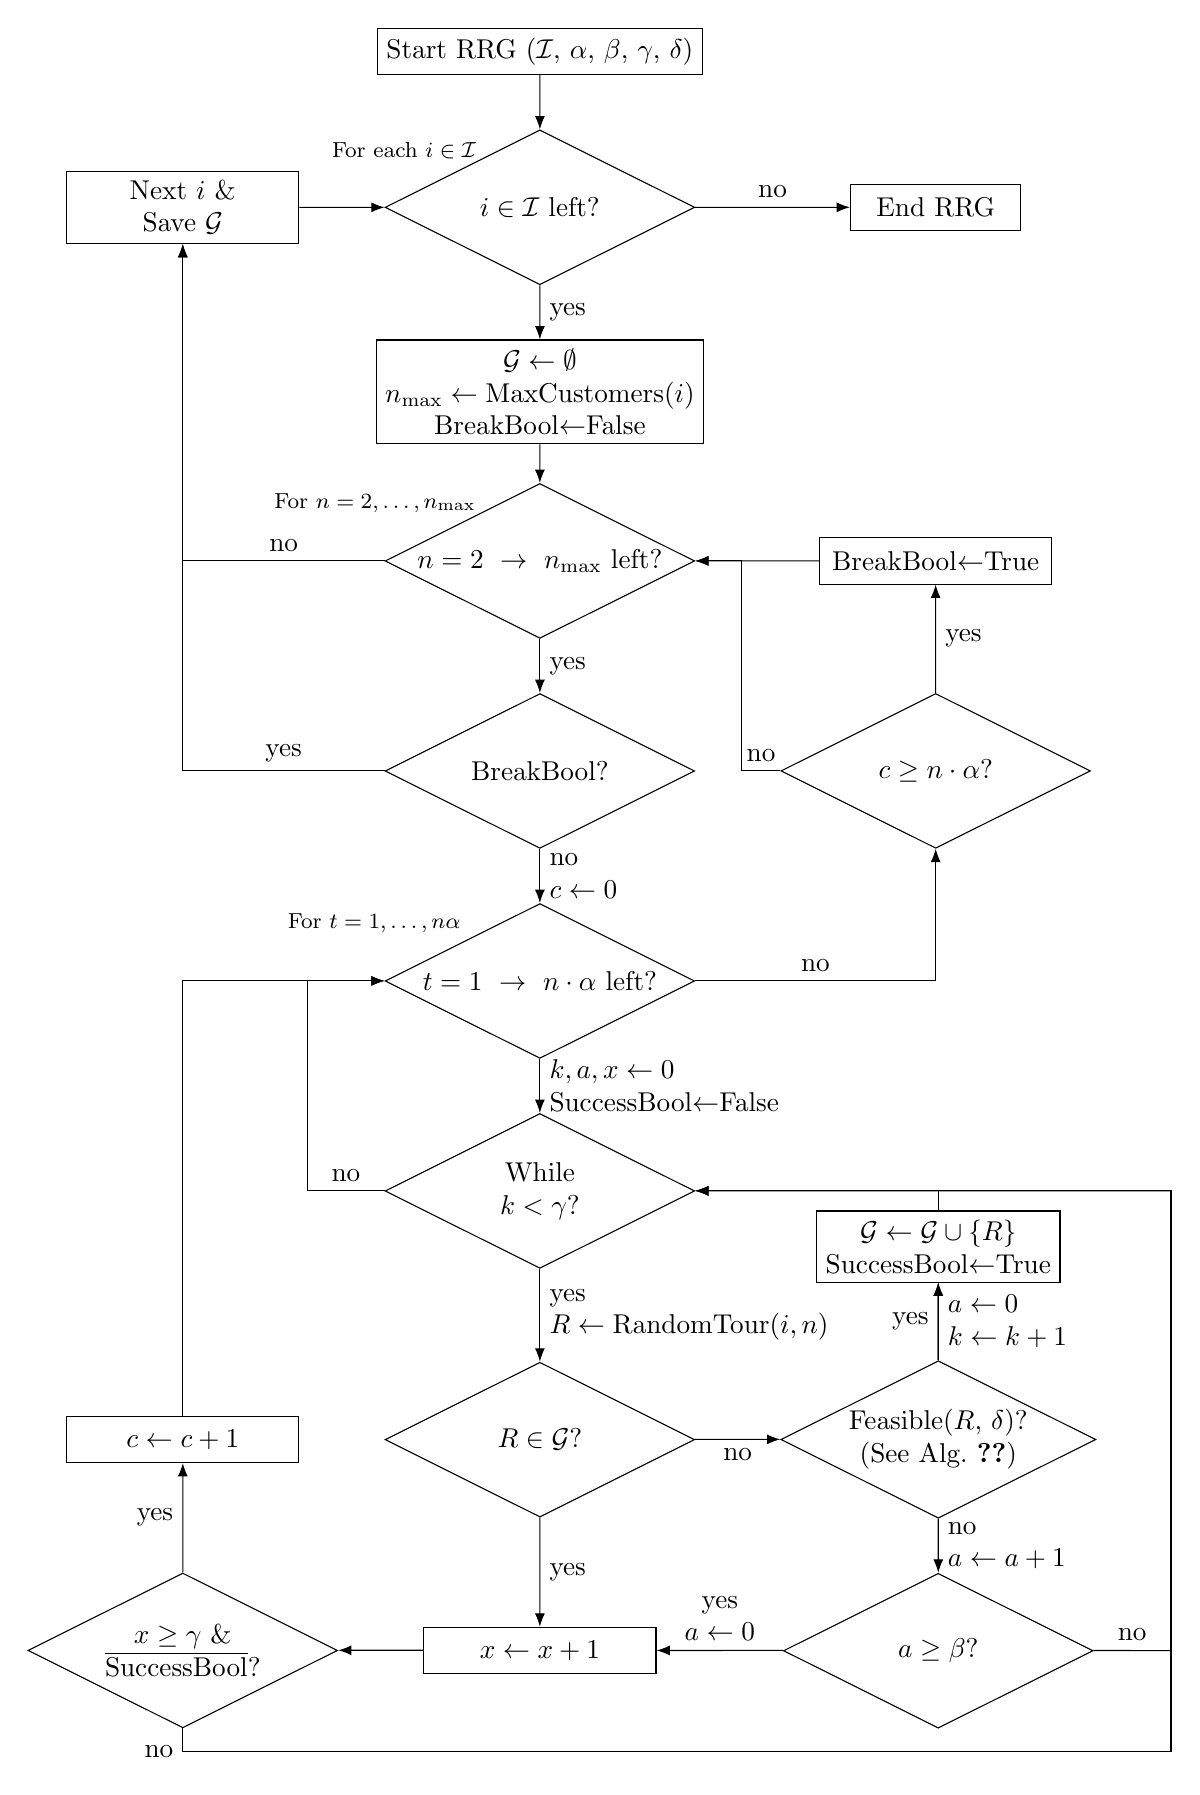
\begin{tikzpicture}[
            scale = 0.983, transform shape,node distance=7mm and 11mm,
            >=Latex,
            % Styles
            startstop/.style   = {rectangle, draw, align=center, minimum width=22mm, minimum height=6mm},
            process/.style     = {rectangle, draw, align=center, minimum width=30mm, minimum height=6mm},
            decision/.style    = {diamond, draw, aspect=2, inner sep=1pt, align=center, minimum width=40mm,minimum height=20mm},
            io/.style          = {trapezium, trapezium left angle=60, trapezium right angle=120, draw, align=center, minimum height=6mm},
            connector/.style   = {circle, draw, inner sep=1pt},
            line/.style        = {->}
        ]

        % Nodes
        \node[startstop] (start) {Start RRG ($\mathcal{I}$, $\alpha$, $\beta$, $\gamma$, $\delta$)};
        \node[decision, below=of start] (forI) {$i\in\mathcal{I}$ left?};
        \node[process, left= of forI] (nextI) {Next $i$ \&\\ Save $\mathcal{G}$};
        \node[process, below=of forI] (initI) {$\mathcal{G}\gets\emptyset$\\$n_{\max}\gets \mathrm{MaxCustomers}(i)$\\BreakBool$\gets$False};
        \node[decision, below=5mm of initI] (forN) {$n=2\ \to\ n_{\max}$ left?};
        \node[decision, below=of forN] (exitOuter) {BreakBool?};
        \node[decision, right=of exitOuter] (breakDec) {$c \geq n \cdot \alpha$?};
        \node[startstop] at ($(breakDec.north |- forI.east)$) (end) {End RRG};
        \node[decision, below=of exitOuter] (forAlpha) {$t=1\ \to\ n\cdot\alpha$ left?};
        \node[decision, below=of forAlpha] (whileK) {While\\$k<\gamma$?};
        \node[decision, below=12 mm of whileK] (dup) {$R\in\mathcal{G}$?};
        % \node[process, bel=of dup] (drawThresh) {$Q^*\gets Q\cdot \mathcal{U}_\delta^1$\\$V^*\gets V\cdot \mathcal{U}_\delta^1$};
        \node[decision, right=of dup] (feasible) {Feasible($R$, $\delta$)?\\(See Alg.~\ref{alg:appendix:check_single_tour})};
        \node[process, above=10mm of feasible] (accept) {$\mathcal{G}\gets \mathcal{G}\cup\{R\}$\\SuccessBool$\gets$True};
        \node[decision, below= of feasible] (attemptCond) {$a\ge \beta$?};
        \node[process] at ($(dup.south |- attemptCond.west)$) (incX) {$x\gets x+1$};
        \node[process, left=of dup] (incC) {$c\gets c+1$};
        \node[decision] at ($(incC.south |- incX.west)$)  (breakCond) {$x\ge \gamma$ \& \\$\overline{\text{SuccessBool}}$?};
        \node[process] at ($(breakDec.north |- forN.east)$) (trueExit) {BreakBool$\gets$True};

        % Edges
        \draw[line] (start) -- (forI);
        \draw[line] (forI) -- node[pos=0.5, right]{yes}(initI);
        \draw[line] (forI) -- node[pos=0.5, above]{no}(end);
        \draw[line] (initI) -- (forN);
        \draw[line] (nextI.east)-- (forI.west);
        \draw[line] (forAlpha.east) -| node[pos = 0.25,above]{no}(breakDec.south);
        \draw[line] (breakDec.west) -- node[pos = 0.5,above]{no}($(breakDec.west)-(5mm,0)$) |- (forN.east);
        \draw[line] (breakDec) -- node[pos = 0.5,right]{yes}(trueExit);
        \draw[line] (trueExit) -- (forN);
        \draw[line] (whileK.west) -- ($(whileK.west)-(10mm,0)$) coordinate (bend) node[pos = 0.5,above]{no} |- (forAlpha.west);

        \draw[line] (forN.south) --  node[pos=0.5, right]{yes}(exitOuter.north);
        \draw[line] (forN.west) -|  node[pos=0.25, above]{no}(nextI.south);
        \draw[line] (exitOuter.west) -| node[pos=0.25, above]{yes} (nextI.south);

        \draw[line] (exitOuter) -- node[pos=0.5, right, align=left]{no\\$c \gets 0$} (forAlpha);

        \draw[line] (forAlpha) -- node[pos=0.5, right, align=left]{$k,a,x\gets 0$\\ SuccessBool$\gets$False} (whileK);
        \draw[line] (whileK) --node[pos=0.5, right, align=left]{yes \\ $R\gets \mathrm{RandomTour}(i,n)$} (dup);
        \draw[line] (dup) -- node[pos=0.5, below]{no}(feasible);
        \draw[line] (dup) -- node[pos=0.5, right]{yes}(incX);
        \draw[line] (incX) -- (breakCond);
        %\draw[line] (breakCond) -- node[pos=0.25, below right]{no}(whileK);
        \draw[line] (breakCond) |- node[pos=0.5, left]{no}($(incX.south)-(0,10mm)$) -| ($(attemptCond.east)+(10mm,0)$) coordinate (bend)|- (whileK);
        \draw[line] (breakCond) -- node[pos=0.5, left]{yes} (incC);
        \draw[line] (incC) |- (forAlpha);

        \draw[line] (feasible) -- node[pos=0.5, left]{yes}(accept);
        \draw[line] (feasible) -- node[pos=0.5, right, align=left]{$a \gets 0$ \\ $k\gets k+1$}(accept);
        \draw[line] (accept.north) |- (whileK.east);

        \draw[line] (feasible) --node[pos=0.5, right, align=left]{no\\$a\gets a+1$} (attemptCond);
        \draw[line] (attemptCond) --node[pos=0.5, above, align=center]{yes\\$a\gets 0$} (incX);
        \draw[line] (attemptCond) -- ($(attemptCond.east)+(10mm,0)$) coordinate (bend) node[pos = 0.5,above]{no} |- (whileK);

        % Labels for the for-loops (optional, visual clarity)
        \node[above left=0mm and -3mm of forI] {\footnotesize For each $i\in\mathcal{I}$};
        \node[above left=0mm and -3mm of forN] {\footnotesize For $n=2,\dots,n_{\max}$};
        \node[above left=0mm and -1mm of forAlpha] {\footnotesize For $t=1,\dots,n\alpha$};

    \end{tikzpicture}
    \caption{Flowchart for Random Routes Generation (RRG).}
    \label{fig:flowchart_randomRouteGeneration}
\end{figure}

\clearpage
\section{Feature Filter Selection}
\label{app:feature_selection}

For the feature selection the presented Algorihm~\ref{alg:filter_algorithm} was used for several levels of the minimum importance threshold
$\epsilon$ excluding low important features and for two different barriers. The aggregated results are shown in the following Figure~\ref{fig:feature_filter_parameters}.
The stacked barplots represent the dictionary count, displaying in green colors the \gls{F-Score} and in blue colors the \gls{MI} score method.
For each stacked feature bar above one of the barriers, the feature is respected in the feature sets, shown in the following Table~\ref{tab:feature_dropsets}.

\begin{figure}[ht]
    \centering
    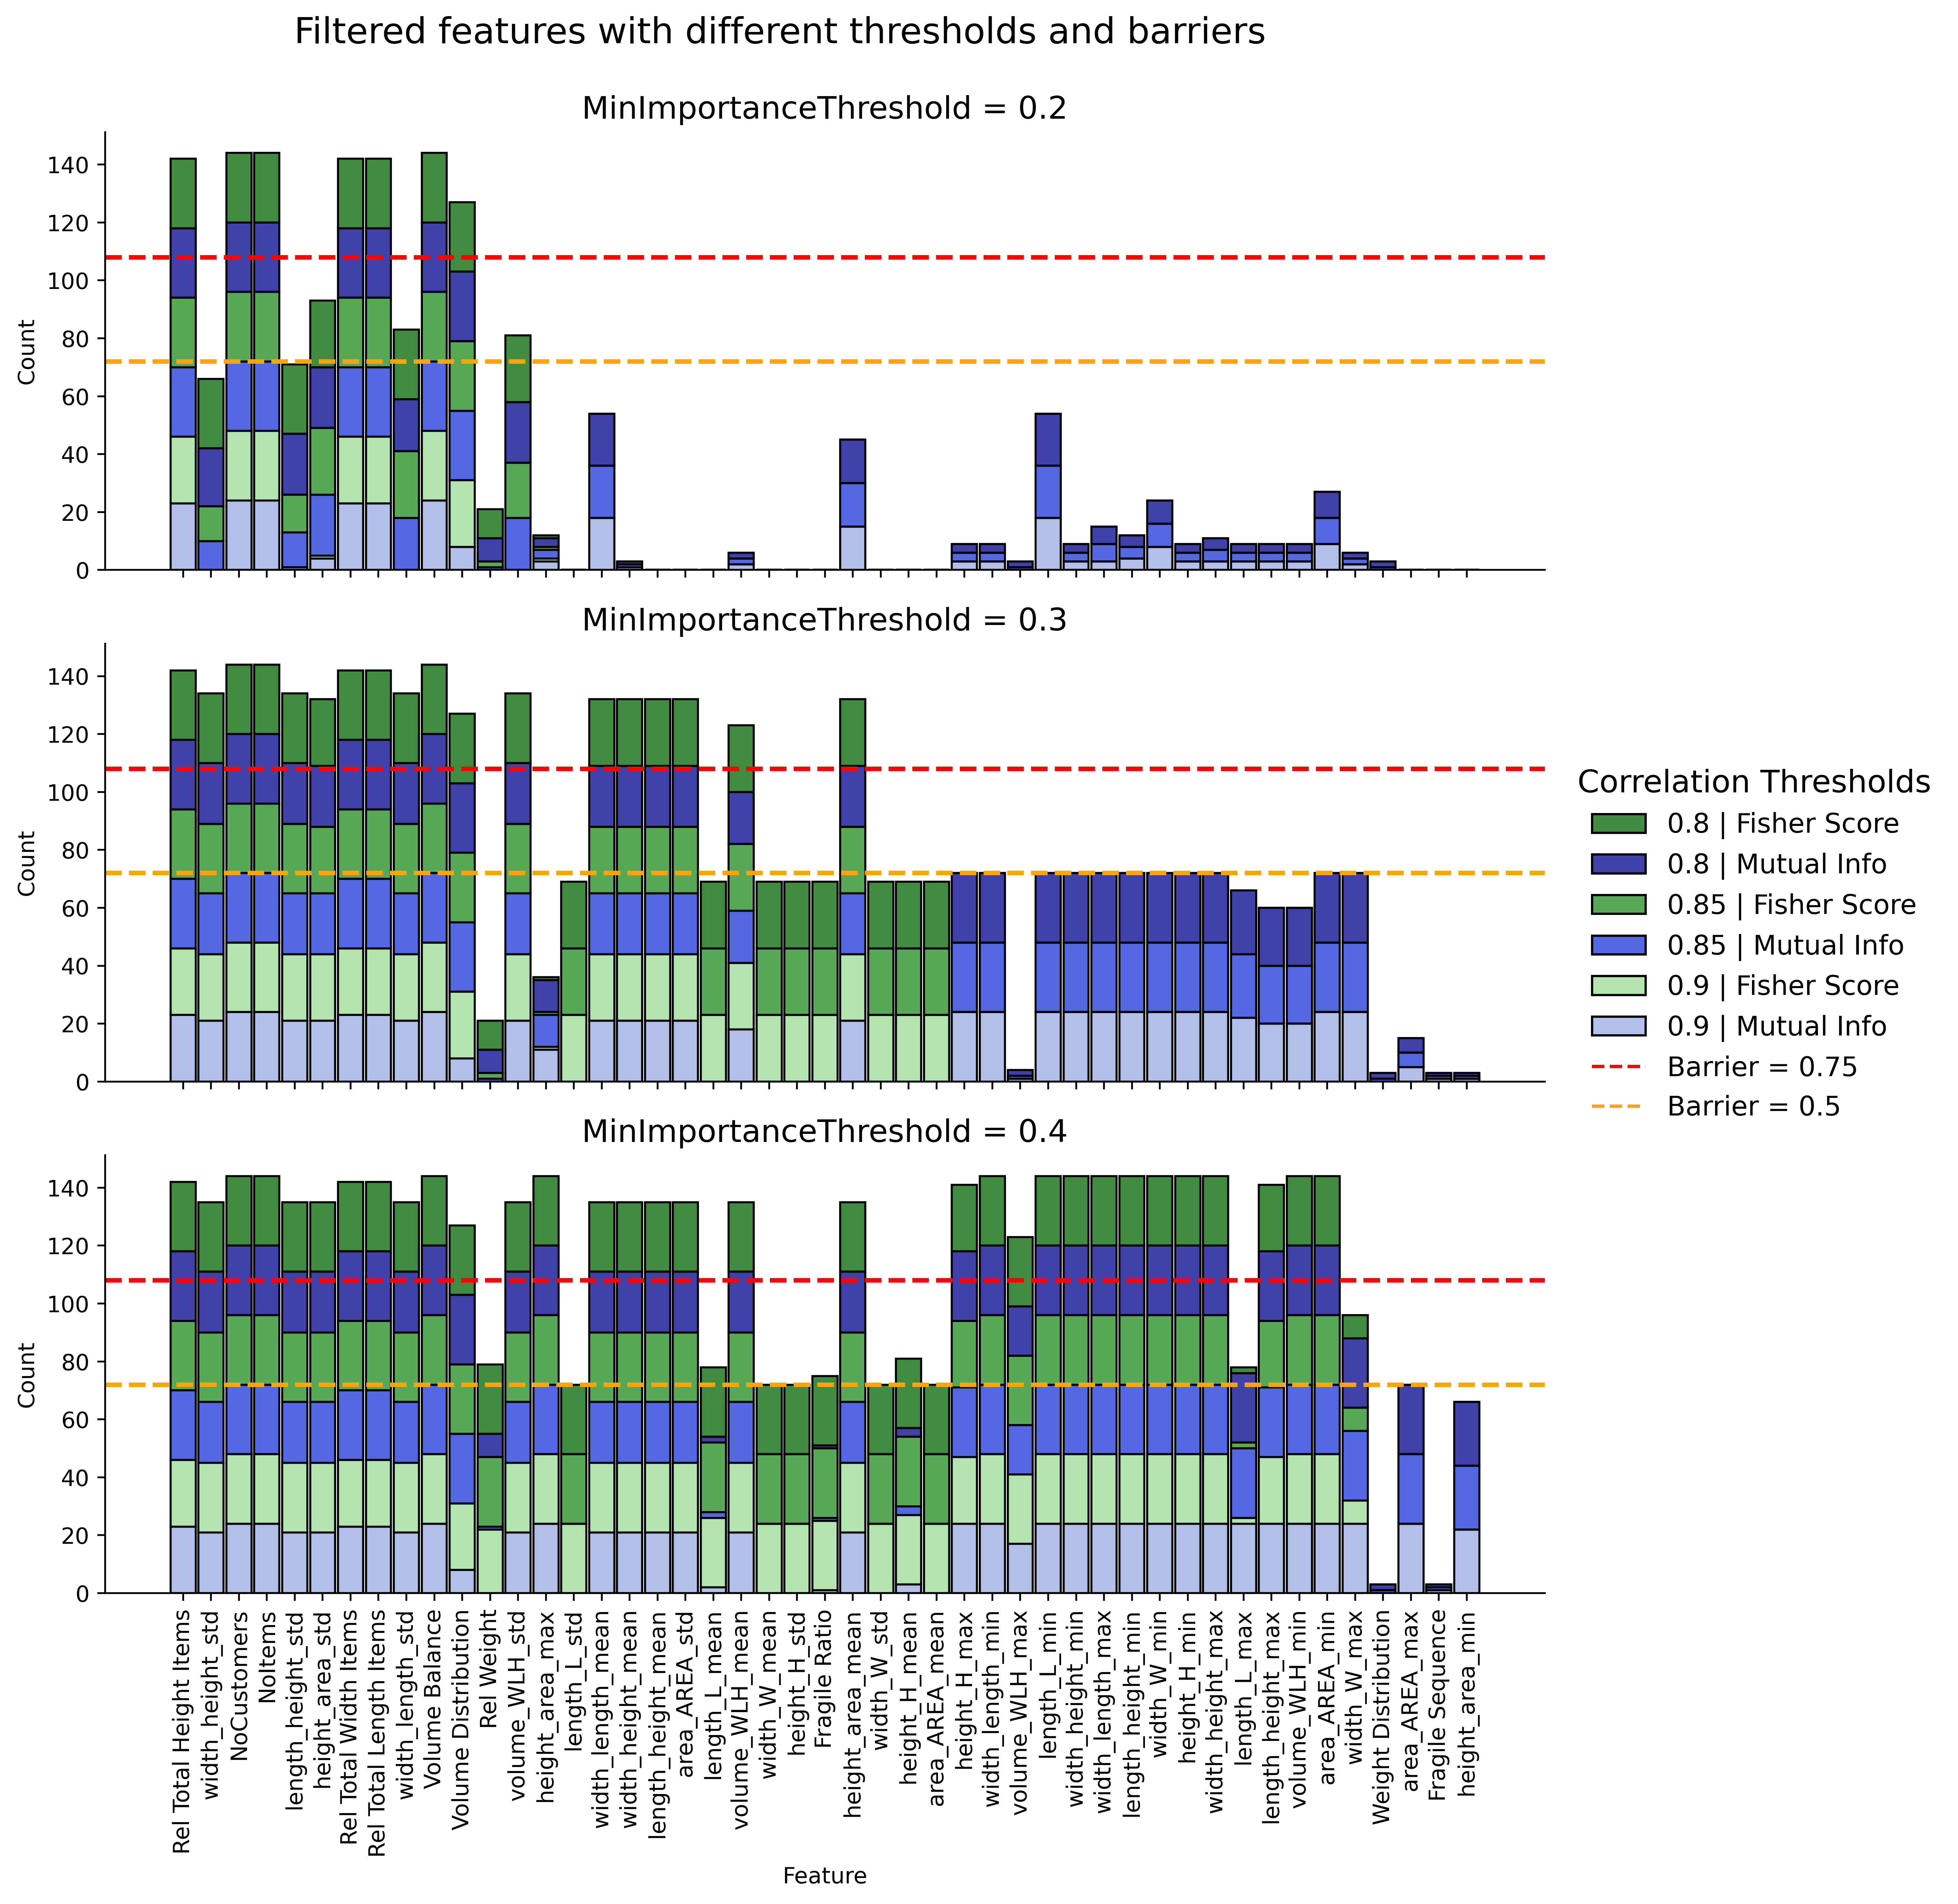
\includegraphics[width=\textwidth,height=0.75\textheight,keepaspectratio]{pictures/feature_filter_facePlot.png}
    \caption{Aggregated results from filter algorithm resulting in different drop sets.}
    \label{fig:feature_filter_parameters}
\end{figure}

\begin{table}[ht]
    \centering
    %\renewcommand{\arraystretch}{1.2}
    \rotatebox{90}{
        \footnotesize
        \begin{tabular}{@{}P{0.04\paperheight}P{0.04\paperheight}P{0.07\paperheight}P{0.05\paperheight}P{0.46\paperheight}@{}}
            \toprule
            Name         & Barrier $B$ & Importance Threshold $\epsilon$ & Number Features & Features                                                                                                                                                                                                                                                                                                                                                                                                                                                                                                                                                                                                                                                      \\
            \midrule
            DropSet-50-2 & 0.50        & 0.2                             & 10              & NoCustomers, NoItems, Rel Total Height Items, Rel Total Length Items, Rel Total Width Items, Volume Balance, Volume Distribution, height-area-std, volume-WLH-std, width-length-std                                                                                                                                                                                                                                                                                                                                                                                                                                                                           \\
            \midrule
            DropSet-50-3 & 0.50        & 0.3                             & 18              & NoCustomers, NoItems, Rel Total Height Items, Rel Total Length Items, Rel Total Width Items, Volume Balance, Volume Distribution, area-AREA-std, height-area-mean, height-area-std, length-height-mean, length-height-std, volume-WLH-mean, volume-WLH-std, width-height-mean, width-height-std, width-length-mean, width-length-std                                                                                                                                                                                                                                                                                                                          \\
            \midrule
            DropSet-50-4 & 0.50        & 0.4                             & 38              & Fragile Ratio, NoCustomers, NoItems, Rel Total Height Items, Rel Total Length Items, Rel Total Width Items, Rel Weight, Volume Balance, Volume Distribution, area-AREA-min, area-AREA-std, height-H-max, height-H-mean, height-H-min, height-area-max, height-area-mean, height-area-std, length-L-max, length-L-mean, length-L-min, length-height-max, length-height-mean, length-height-min, length-height-std, volume-WLH-max, volume-WLH-mean, volume-WLH-min, volume-WLH-std, width-W-max, width-W-min, width-height-max, width-height-mean, width-height-min, width-height-std, width-length-max, width-length-mean, width-length-min, width-length-std \\
            \midrule
            DropSet-75-2 & 0.50        & 0.2                             & 7               & NoCustomers, NoItems, Rel Total Height Items, Rel Total Length Items, Rel Total Width Items, Volume Balance, Volume Distribution                                                                                                                                                                                                                                                                                                                                                                                                                                                                                                                              \\
            \midrule
            DropSet-75-3 & 0.50        & 0.3                             & 18              & NoCustomers, NoItems, Rel Total Height Items, Rel Total Length Items, Rel Total Width Items, Volume Balance, Volume Distribution, area-AREA-std, height-area-mean, height-area-std, length-height-mean, length-height-std, volume-WLH-mean, volume-WLH-std, width-height-mean, width-height-std, width-length-mean, width-length-std                                                                                                                                                                                                                                                                                                                          \\
            \midrule
            DropSet-75-4 & 0.50        & 0.4                             & 32              & NoCustomers, NoItems, Rel Total Height Items, Rel Total Length Items, Rel Total Width Items, Volume Balance, Volume Distribution, area-AREA-min, area-AREA-std, height-H-max, height-H-min, height-area-max, height-area-mean, height-area-std, length-L-min, length-height-max, length-height-mean, length-height-min, length-height-std, volume-WLH-max, volume-WLH-mean, volume-WLH-min, volume-WLH-std, width-W-min, width-height-max, width-height-mean, width-height-min, width-height-std, width-length-max, width-length-mean, width-length-min, width-length-std                                                                                     \\

            \bottomrule
        \end{tabular}}
    \caption{Feature dropsets with different parameter combinations of $\epsilon$ and $B$.}
    \label{tab:feature_dropsets}
\end{table}

\begin{table}[ht]
    \centering
    \small
    \caption{Model hyperparameters for feature selection.}
    \label{tab:hyperparams_feature_selection}
    \renewcommand{\arraystretch}{1.1}
    \begin{tabular}{@{}c P{0.3\textwidth}P{0.3\textwidth}@{}}
        \toprule
        \textbf{LR}                  & \textbf{XGB}                    & \textbf{FFNN}                      \\
        \midrule
        \kv{penalty}{l2}             & \kv{objective}{binary:logistic} & \kv{hidden\_layers}{[128, 64, 32]} \\
        \kv{C}{1.0}                  & \kv{eval\_metric}{logloss}      & \kv{dropout}{0.2}                  \\
        \kv{solver}{lbfgs}           & \kv{max\_depth}{15}             & \kv{lr}{0.001}                     \\
        \kv{max\_iter}{1000}         & \kv{n\_estimators}{500}         & \kv{batch\_size}{512}              \\
        \kv{class\_weight}{balanced} & \kv{learning\_rate}{0.05}       & \kv{epochs}{50}                    \\
        \kv{random\_state}{42}       & \kv{subsample}{0.8}             & \kv{pos\_weight}{null}             \\
        \kv{n\_jobs}{23}             & \kv{colsample\_bytree}{0.8}     & \kv{weight\_decay}{0.0}            \\
                                     & \kv{reg\_alpha}{0.0}            & \kv{batch\_size}{512}              \\
                                     & \kv{reg\_lambda}{1.0}           & \kv{device}{cpu}                   \\
                                     & \kv{enable\_categorical}{false} & \kv{random\_state}{42}             \\
                                     & \kv{tree\_method}{hist}         & \kv{n\_jobs}{23}                   \\
                                     & \kv{n\_jobs}{23}                &                                    \\
                                     & \kv{random\_state}{42}          &                                    \\
        \bottomrule
    \end{tabular}
\end{table}

\clearpage
\section{Parking Lot}
\label{app:trash}
With a subset from krebs the following datasets were created!
\begin{table}[ht]
    \centering
    \begin{tabular}{c c cc c c c}
        \hline
        \makecell{Multiplier $\alpha$} & \makecell{Attempts                          \\ limit $\beta$} & \makecell{Success \\threshold $\gamma$} & Routes & Balance& \gls{MCC}-Score & F1-Score \\
        \hline
        1                              & 1                  & 1 & 7616  & 60/40 &  & \\
        1                              & 1                  & 2 & 15948 & 60/40 &  & \\
        1                              & 1                  & 3 & 24573 & 60/40 &  & \\
        1                              & 2                  & 1 & 8325  & 60/40 &  & \\
        1                              & 2                  & 2 & 17217 & 60/40 &  & \\
        1                              & 2                  & 3 & 26467 & 60/40 &  & \\
        1                              & 3                  & 1 & 8683  & 60/40 &  & \\
        1                              & 3                  & 2 & 18041 & 60/40 &  & \\
        1                              & 3                  & 3 & 27535 & 60/40 &  & \\
        \hline
    \end{tabular}
    \caption[Created instances for different parameter combinations $(\alpha, \beta, \gamma)$ for \krebsADataSetText dataset.]{Created instances for different parameter combinations $(\alpha, \beta, \gamma)$ for \krebsADataSetText dataset.
        The values in the balance column stand for the share of positive and netative labels in the sample population.}
    \label{tab:created_instances_xyz_krebs}
\end{table}



\begin{table}[ht]
    \centering
    \begin{tabular}{c c c c c c}
        \toprule
        Model                          & Name     & \gls{MCC}-Score & \gls{AUROC} & F1-Score & Accuracy \\
        \midrule
        \multirow{3}{*}{\gls{LR}}      & Complete & 0.6             & 0.9         & 0.87     & 0.95     \\
                                       & Trimmed  & 0.6             & 0.9         & 0.87     & 0.95     \\
                                       & Shrinked & 0.6             & 0.9         & 0.87     & 0.95     \\
        \midrule
        \multirow{3}{*}{Decision Tree} & Complete & 0.6             & 0.9         & 0.87     & 0.95     \\
                                       & Trimmed  & 0.6             & 0.9         & 0.87     & 0.95     \\
                                       & Shrinked & 0.6             & 0.9         & 0.87     & 0.95     \\
        \midrule
        \multirow{3}{*}{\gls{FFNN}}    & Complete & 0.6             & 0.9         & 0.87     & 0.95     \\
                                       & Trimmed  & 0.6             & 0.9         & 0.87     & 0.95     \\
                                       & Shrinked & 0.6             & 0.9         & 0.87     & 0.95     \\
        \bottomrule
    \end{tabular}
    \caption{Results}
    \label{tab:dataset_model_selection_saveStrategy}
\end{table}

\begin{table}[ht]
    \centering
    \begin{tabular}{c c c c c c}
        \toprule
        Model                           & Name       & \gls{MCC}-Score & \gls{AUROC} & F1-Score & Accuracy \\
        \midrule
        \multirow{13}{*}{\gls{LR}}      & RD-2-20-20 & 0.6             & 0.9         & 0.87     & 0.95     \\
                                        & RD-2-20-30 & 0.6             & 0.9         & 0.87     & 0.95     \\
                                        & RD-2-30-20 & 0.6             & 0.9         & 0.87     & 0.95     \\
                                        & RD-2-30-30 & 0.6             & 0.9         & 0.87     & 0.95     \\
                                        & RD-3-20-20 & 0.6             & 0.9         & 0.87     & 0.95     \\
                                        & RD-3-20-30 & 0.6             & 0.9         & 0.87     & 0.95     \\
                                        & RD-3-30-20 & 0.6             & 0.9         & 0.87     & 0.95     \\
                                        & RD-3-30-30 & 0.6             & 0.9         & 0.87     & 0.95     \\
                                        & RD-4-20-20 & 0.6             & 0.9         & 0.87     & 0.95     \\
                                        & RD-4-20-30 & 0.6             & 0.9         & 0.87     & 0.95     \\
                                        & RD-4-30-20 & 0.6             & 0.9         & 0.87     & 0.95     \\
                                        & RD-4-30-30 & 0.6             & 0.9         & 0.87     & 0.95     \\
                                        & RD-5-40-40 & 0.6             & 0.9         & 0.87     & 0.95     \\
        \midrule
        \multirow{13}{*}{Decision Tree} & RD-2-20-20 & 0.6             & 0.9         & 0.87     & 0.95     \\
                                        & RD-2-20-30 & 0.6             & 0.9         & 0.87     & 0.95     \\
                                        & RD-2-30-20 & 0.6             & 0.9         & 0.87     & 0.95     \\
                                        & RD-2-30-30 & 0.6             & 0.9         & 0.87     & 0.95     \\
                                        & RD-3-20-20 & 0.6             & 0.9         & 0.87     & 0.95     \\
                                        & RD-3-20-30 & 0.6             & 0.9         & 0.87     & 0.95     \\
                                        & RD-3-30-20 & 0.6             & 0.9         & 0.87     & 0.95     \\
                                        & RD-3-30-30 & 0.6             & 0.9         & 0.87     & 0.95     \\
                                        & RD-4-20-20 & 0.6             & 0.9         & 0.87     & 0.95     \\
                                        & RD-4-20-30 & 0.6             & 0.9         & 0.87     & 0.95     \\
                                        & RD-4-30-20 & 0.6             & 0.9         & 0.87     & 0.95     \\
                                        & RD-4-30-30 & 0.6             & 0.9         & 0.87     & 0.95     \\
                                        & RD-5-40-40 & 0.6             & 0.9         & 0.87     & 0.95     \\
        \midrule
        \multirow{13}{*}{\gls{FFNN}}    & RD-2-20-20 & 0.6             & 0.9         & 0.87     & 0.95     \\
                                        & RD-2-20-30 & 0.6             & 0.9         & 0.87     & 0.95     \\
                                        & RD-2-30-20 & 0.6             & 0.9         & 0.87     & 0.95     \\
                                        & RD-2-30-30 & 0.6             & 0.9         & 0.87     & 0.95     \\
                                        & RD-3-20-20 & 0.6             & 0.9         & 0.87     & 0.95     \\
                                        & RD-3-20-30 & 0.6             & 0.9         & 0.87     & 0.95     \\
                                        & RD-3-30-20 & 0.6             & 0.9         & 0.87     & 0.95     \\
                                        & RD-3-30-30 & 0.6             & 0.9         & 0.87     & 0.95     \\
                                        & RD-4-20-20 & 0.6             & 0.9         & 0.87     & 0.95     \\
                                        & RD-4-20-30 & 0.6             & 0.9         & 0.87     & 0.95     \\
                                        & RD-4-30-20 & 0.6             & 0.9         & 0.87     & 0.95     \\
                                        & RD-4-30-30 & 0.6             & 0.9         & 0.87     & 0.95     \\
                                        & RD-5-40-40 & 0.6             & 0.9         & 0.87     & 0.95     \\
        \bottomrule
    \end{tabular}
    \caption{Results}
    \label{tab:dataset_model_selection_randomStrategy}
\end{table}

\clearpage


\section{Parameterstudy}

\subsection{NoClasifier Variant}
\label{app:subsec:parameterstudy_noclassifier}

\begin{figure}[!ht]
    \centering
    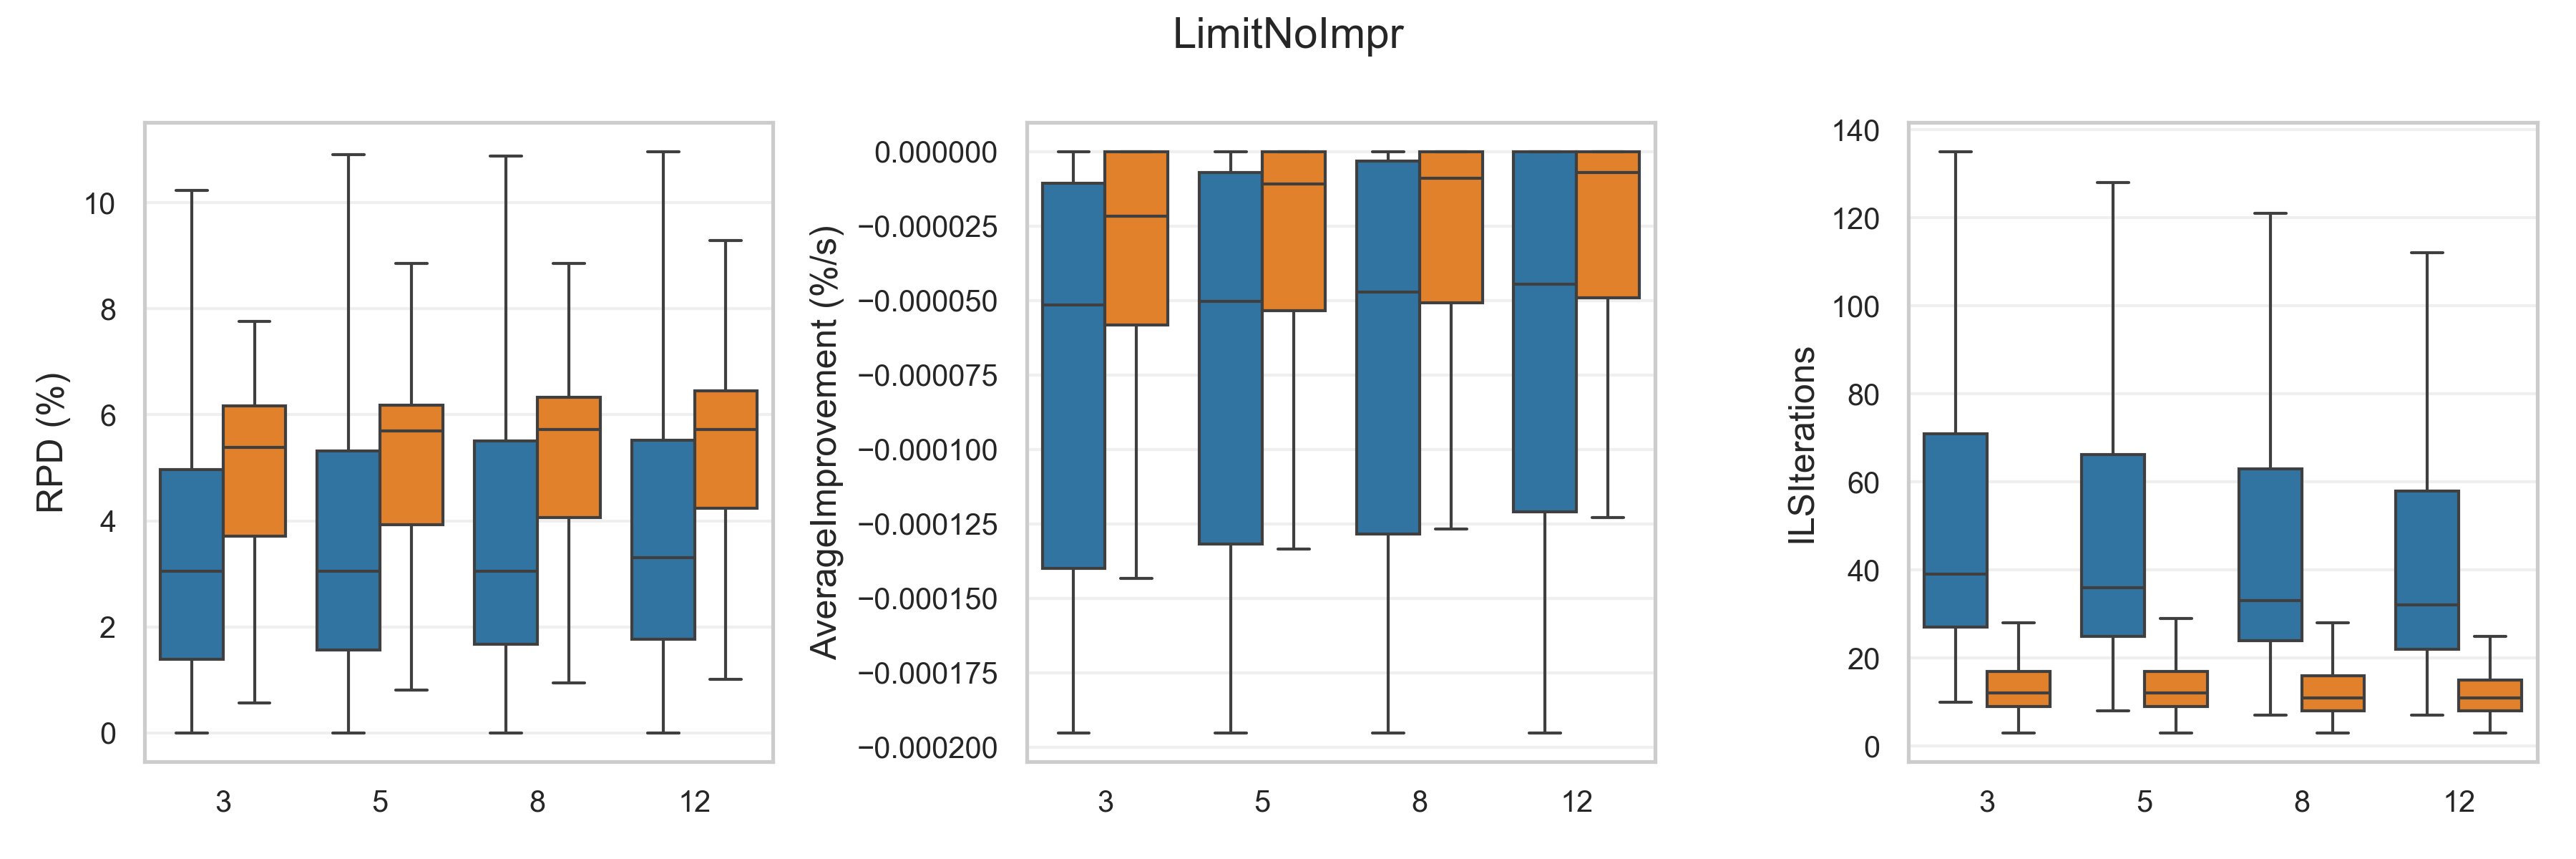
\includegraphics[width=\textwidth]{pictures/LimitNoImpr_base_parameter_study.png}
    \caption{Parameterstudy of LimitNoImpr divided in two groups based on the average iterations.}
    \label{fig:parameterstudy_NoClassifier_limitNoImpr}
\end{figure}

\begin{figure}[!ht]
    \centering
    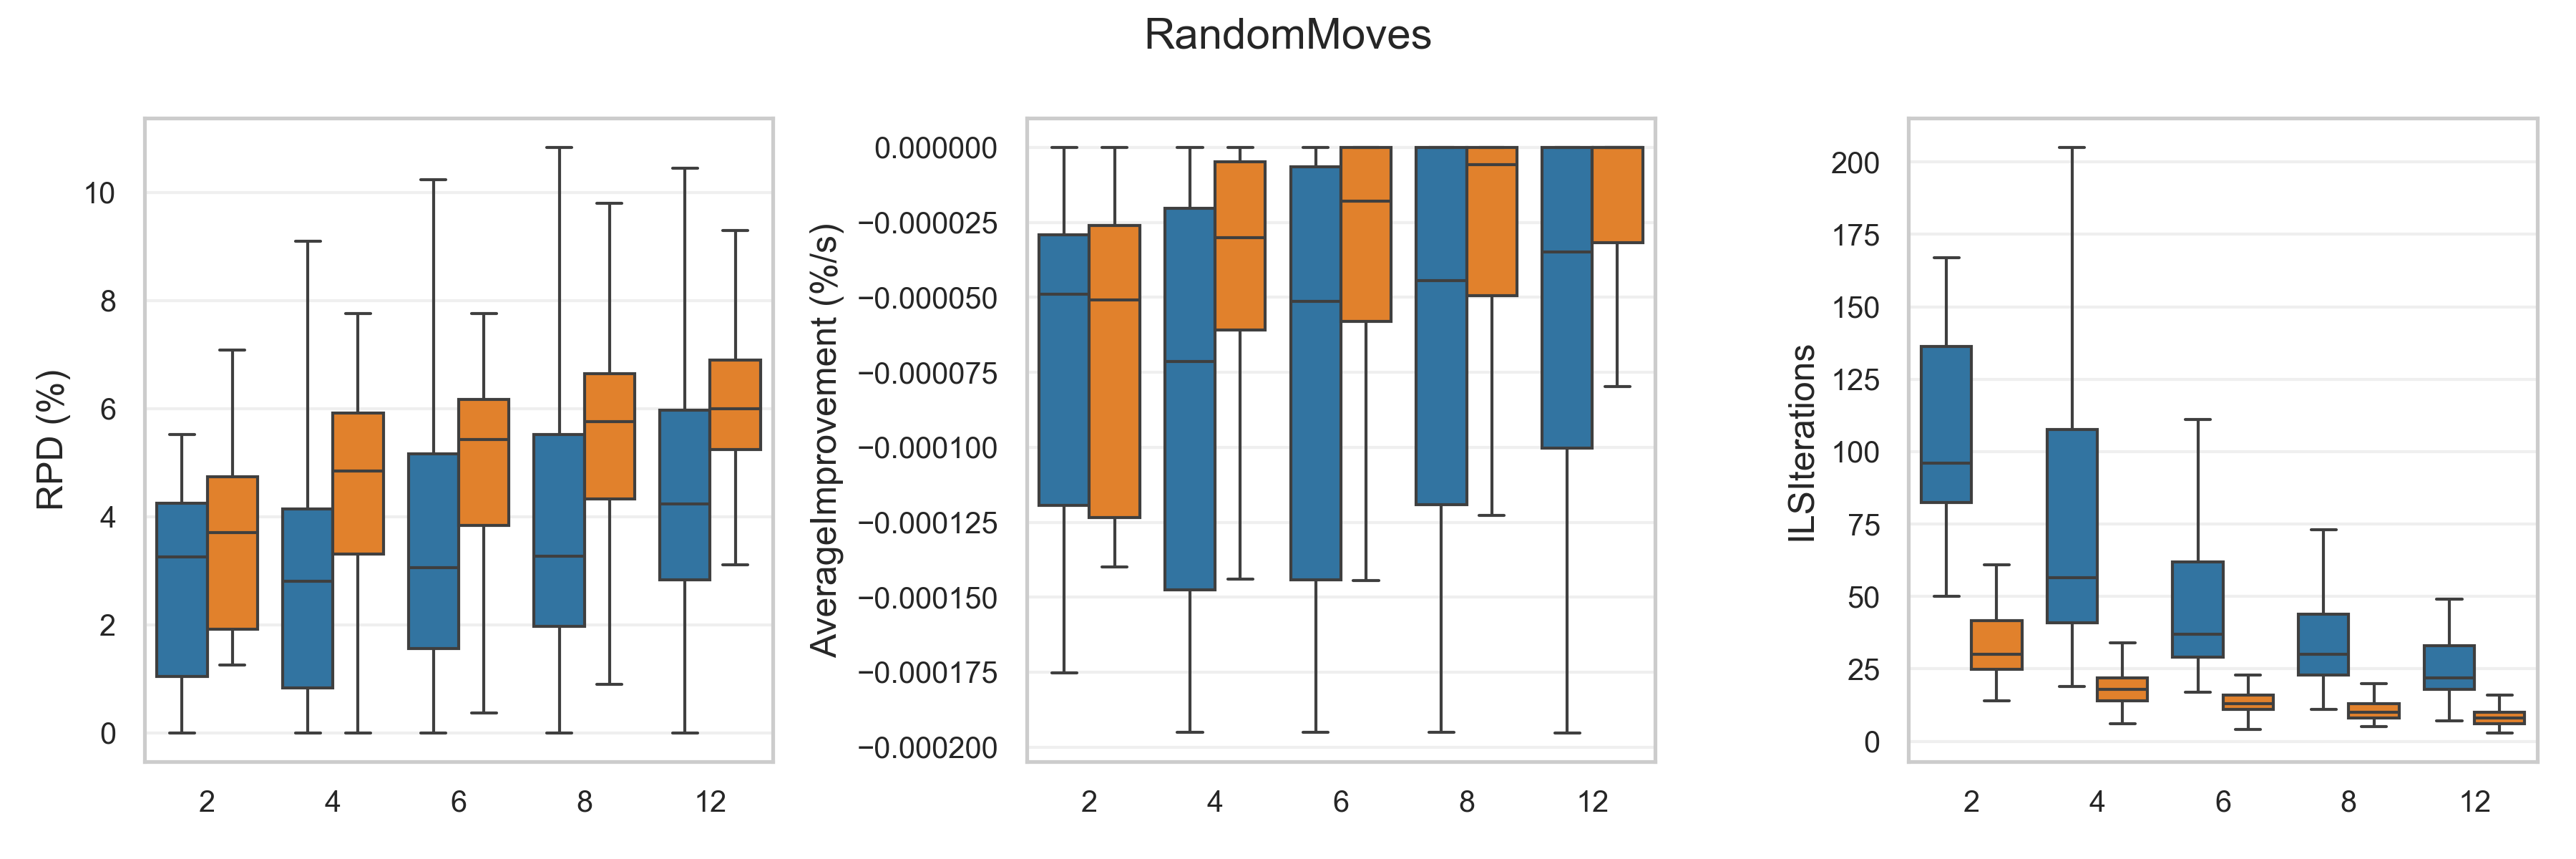
\includegraphics[width=\textwidth]{pictures/RandomMoves_base_parameter_study.png}
    \caption{Parameterstudy of RandomMoves divided in two groups based on the average iterations.}
    \label{fig:parameterstudy_NoClassifier_RandomMoves}
\end{figure}

\begin{figure}[!ht]
    \centering
    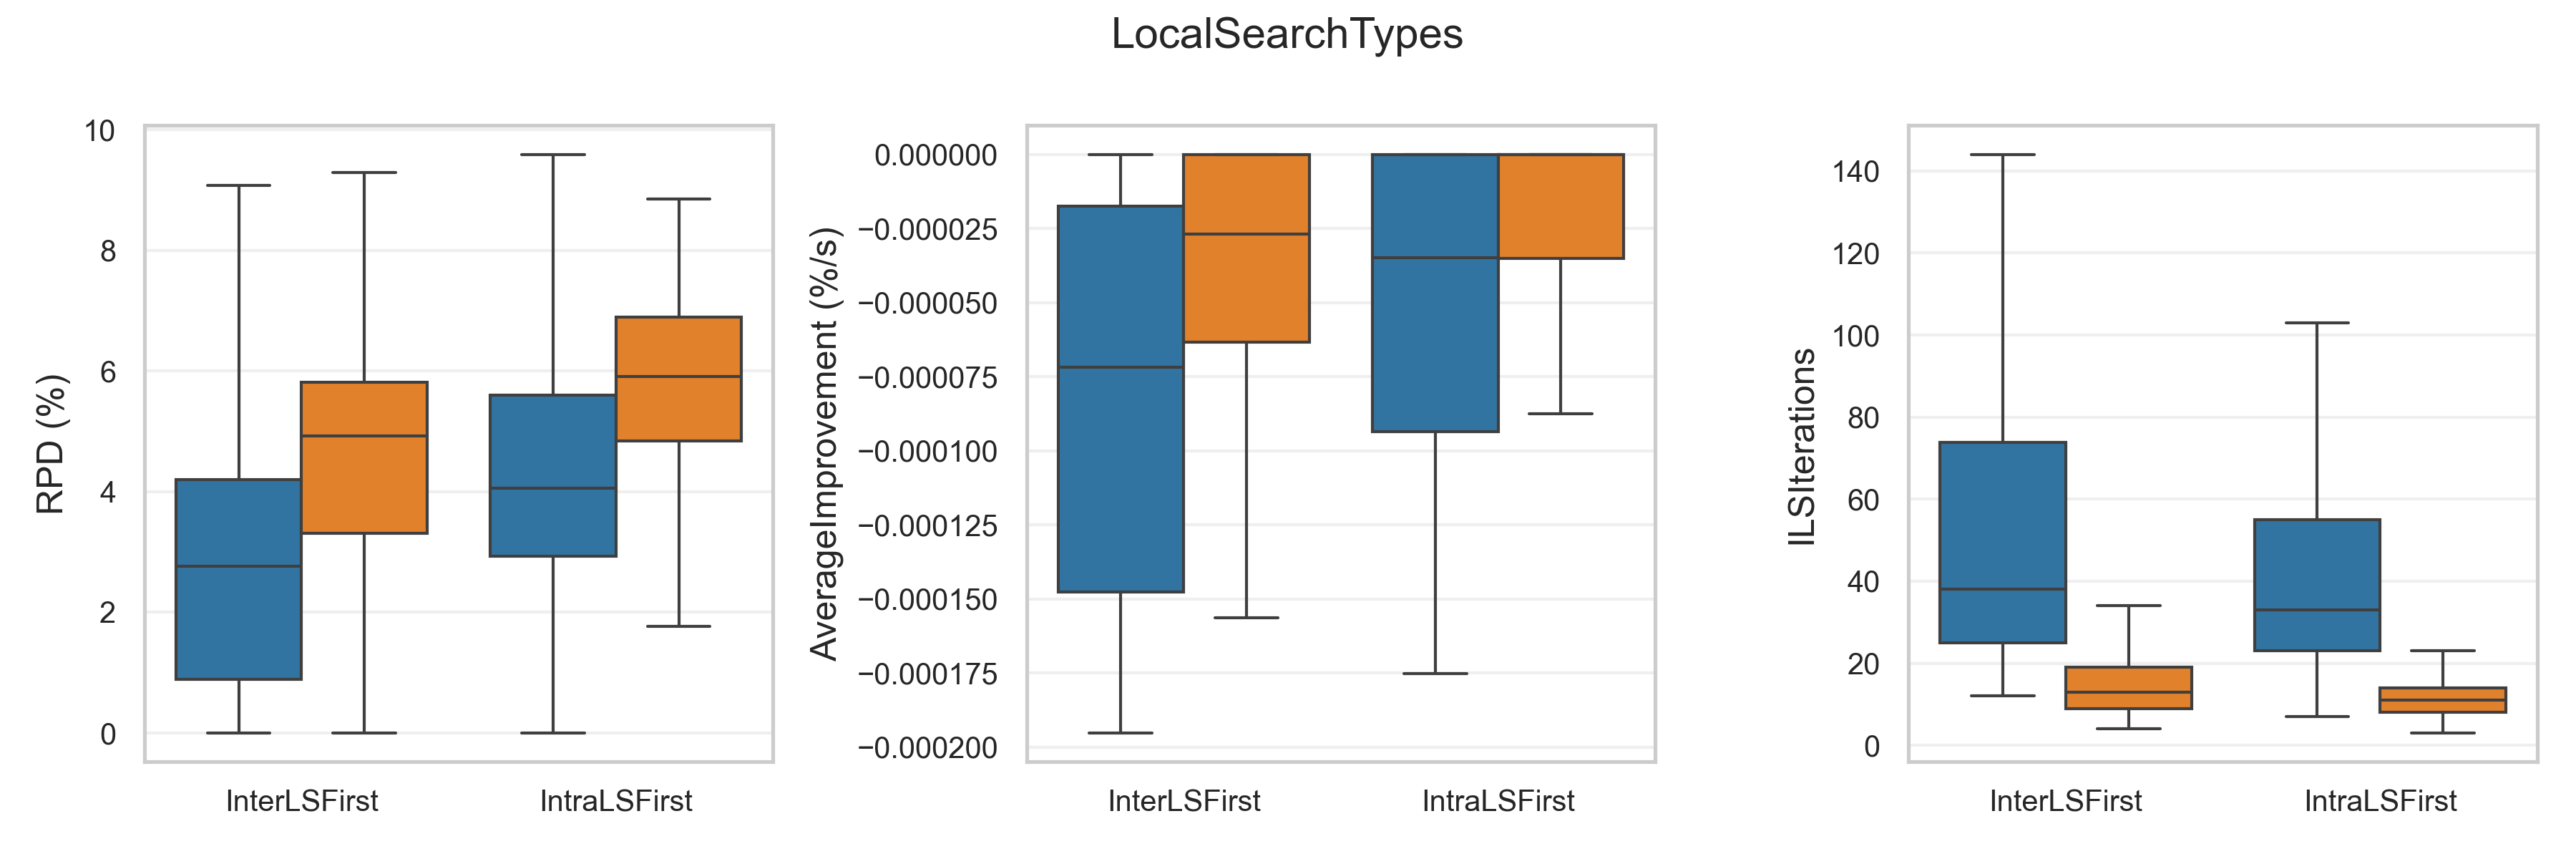
\includegraphics[width=\textwidth]{pictures/LocalSearchTypes_base_parameter_study.png}
    \caption{Parameterstudy of the order of local search neighborhoods divided in two groups based on the average iterations.}
    \label{fig:parameterstudy_NoClassifier_localSearch}
\end{figure}

\begin{figure}[!ht]
    \centering
    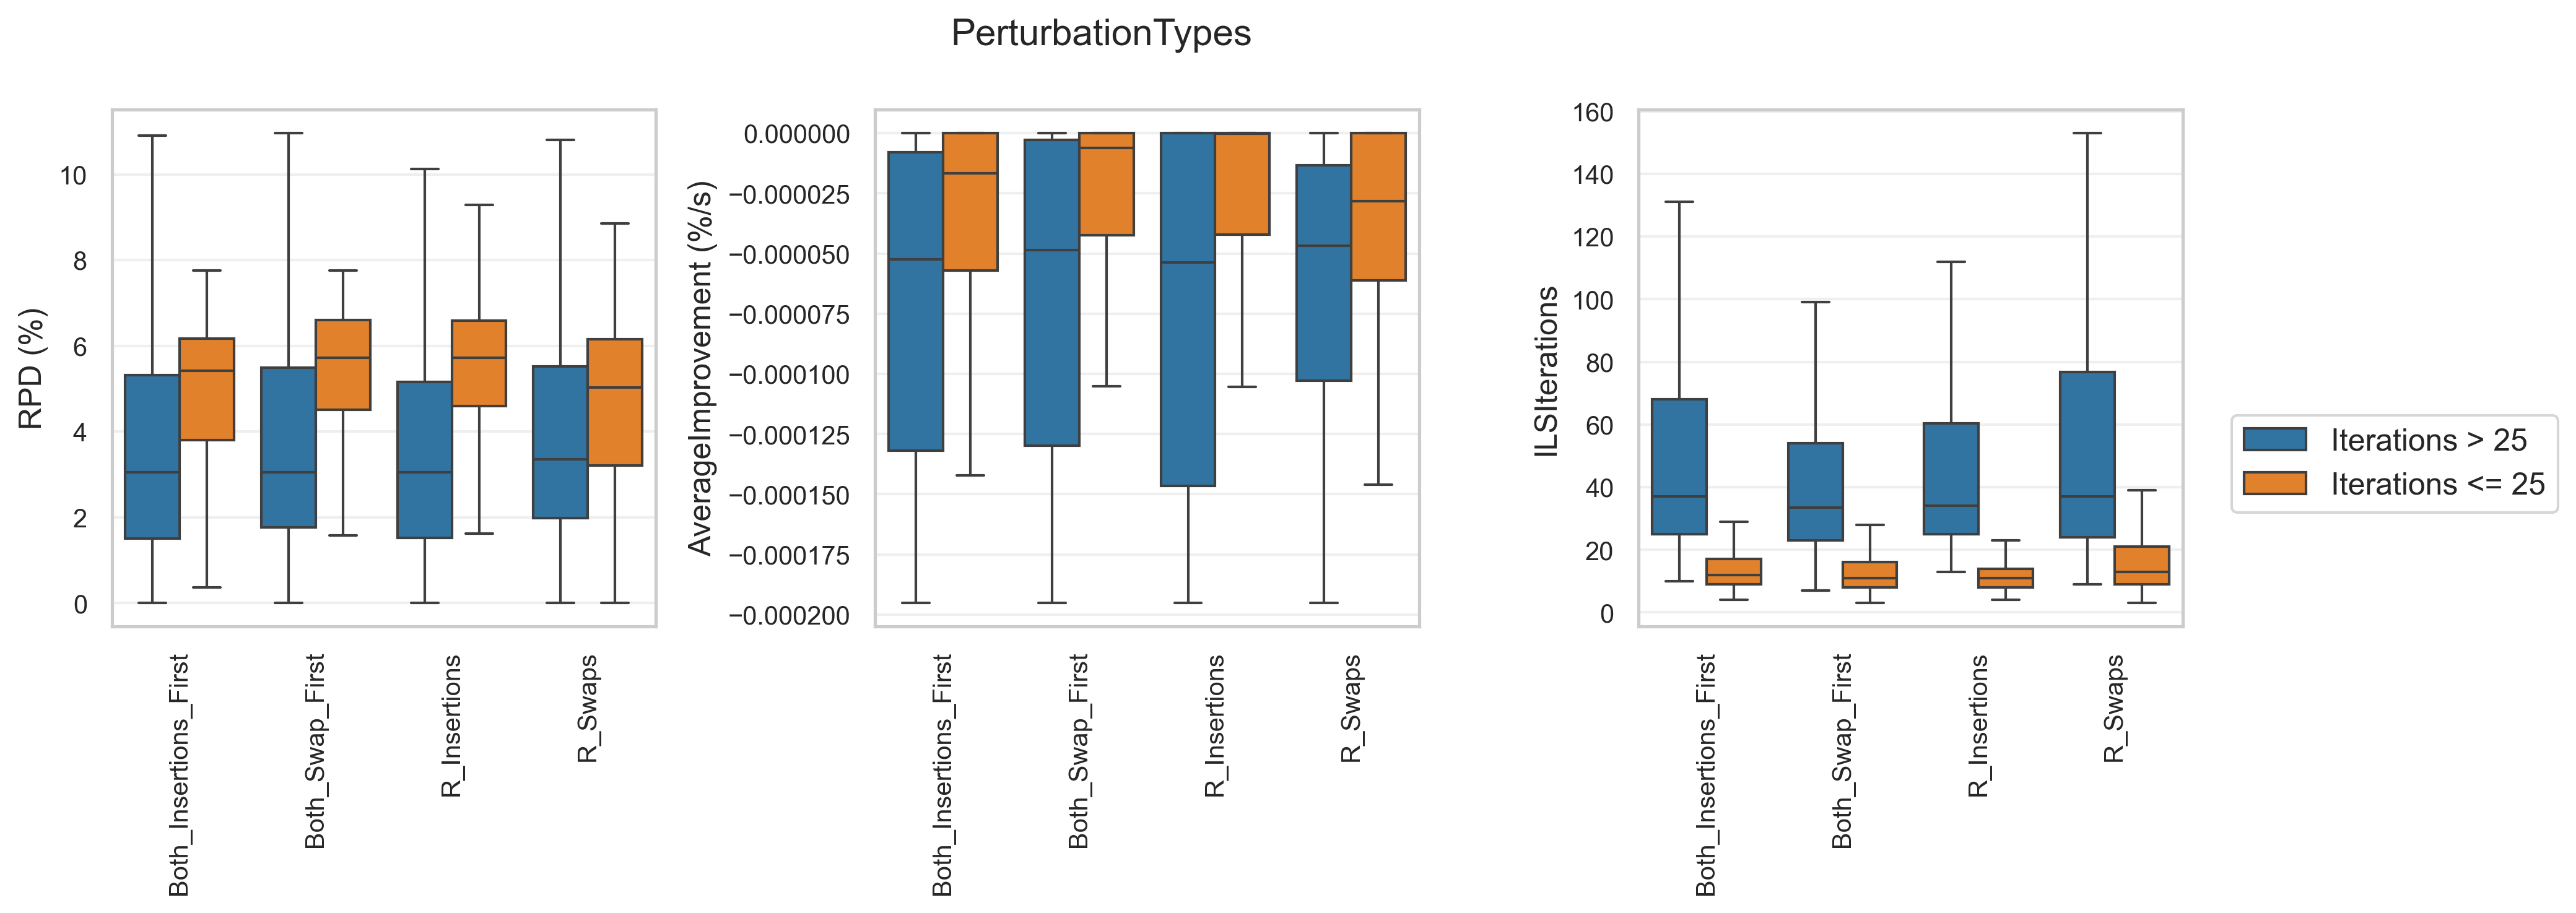
\includegraphics[width=\textwidth]{pictures/PerturbationTypes_base_parameter_study.png}
    \caption{Parameterstudy of the set and order of perturbation neighborhoods divided in two groups based on the average iterations.}
    \label{fig:parameterstudy_NoClassifier_perturbation}
\end{figure}

\subsection{SpeedUp Variant}
\label{app:subsec:parameterstudy_SpeedUp}


\clearpage
%####################### Literaturverzeichnis #########################
\addcontentsline{toc}{chapter}{\bibname}
\printbibliography
%####################### Selbständigkeitserklärung ####################

\newConfirmationEnglish{Dresden}

%####################### Platzhalter - Abkürzungsverzeichnis muss erstellt werden####################

%\printacronyms[style=bwlimsuper]

%####################### End of Document ####################
\end{document}